\documentclass[aspectratio=169,11pt,usenames,dvipsnames]{beamer}

% \usepackage[colorlinks=true,linkcolor=customblue, citecolor=hpred,urlcolor=customlightblue]{hyperref}

% theme
\usetheme{simple}

% packages
\usepackage{mathrsfs}  
\usepackage{cancel}
% \usepackage{caption}
% \usepackage{tikz}

\setbeamercovered{transparent}
\usepackage{tikz}
\usetikzlibrary{overlay-beamer-styles}
 \tikzset{
    highlight on/.style={alt={#1{fill=customblue!80!black,color=customblue!80!black}{fill=gray!30!white,color=gray!30!white}}},
}
\usetikzlibrary{shapes}
\usetikzlibrary{plotmarks}

\usetikzlibrary{arrows.meta,
                decorations.pathreplacing,
                    calligraphy,
                tikzmark}

% \usepackage[symbol]{footmisc}
% \renewcommand*{\thefootnote}{\fnsymbol{*}}
\makeatother
\renewcommand{\thefootnote}{$\star$}
\makeatletter

\newcommand\blfootnote[1]{%
  \begingroup
  \renewcommand\thefootnote{}\footnote{#1}%
  \addtocounter{footnote}{-1}%
  \endgroup
}

\usepackage{xcolor}
\usepackage{graphicx}
\usepackage{empheq}
\usepackage{physics}
\usepackage{svg}
\usepackage{bm}
% \usepackage{esvect}
% \usepackage{emoji}
\usepackage{annotate-equations}

% back-up slides
\usepackage{appendixnumberbeamer}

\usepackage{relsize}

% \usepackage{unicode-math}



\usetikzlibrary{decorations.pathreplacing, decorations.pathmorphing,calc,arrows,positioning}

% Custom colors
\definecolor{lightcustomblue}{HTML}{aad1e6}
% \definecolor{lightcustomblue}{HTML}{d8bcc1}
\definecolor{customblue}{HTML}{3c9bb3}
\definecolor{isred}{HTML}{81182d}
\definecolor{hpred}{HTML}{712A27}

% \definecolor{customgreen}{HTML}{8B9556}
% ming
\definecolor{customgreen}{HTML}{117877}

% \definecolor{custompink}{HTML}{CC8B8C}
% pinky
\definecolor{custompink}{HTML}{c35861}
\definecolor{lightpink}{HTML}{ba8489}

\definecolor{starrymain}{HTML}{3B5B65}
\definecolor{starrysecond}{HTML}{719593}
\definecolor{hpblue}{HTML}{44545c}

\definecolor{ektgreen}{HTML}{047c73}
\definecolor{ektblue}{HTML}{065680}

\definecolor{angcorr}{HTML}{502d7e}

\definecolor{pinky}{HTML}{c35861}
\definecolor{ming}{HTML}{117877}

\definecolor{customred}{HTML}{9d1700}
% \definecolor{customyellow}{HTML}{ebcc2a}
\definecolor{customyellow}{HTML}{e0ad04}
\definecolor{lightgray}{HTML}{a6a4a4}

\definecolor{jyublue}{HTML}{002145}
\definecolor{jyured}{HTML}{e13126}
\definecolor{jyulightblue}{HTML}{909eae}

\hypersetup{colorlinks,linkcolor=normal,citecolor=customblue, citecolor=pinky,urlcolor=pinky}

% bibliography
% \usepackage[style=numeric]{biblatex}
% \addbibresource{references.bib}

% custom commands
\newcommand{\coloredeq}[2]{\begin{empheq}[box=\colorbox{#1}]{align*}#2\end{empheq}}
\newcommand\scalemath[2]{\scalebox{#1}{\mbox{\ensuremath{\displaystyle #2}}}}
\newcommand\coloreditem[1]{\item[\textcolor{#1}{\usebeamertemplate{itemize \beameritemnestingprefix item}}]}
\newcommand{\imp}[1]{{\sffamily\bfseries\color{customblue}#1}}

\setbeamertemplate{frametitle}[default][center]


% centered toc
% \newsavebox{\longestsec}

\usepackage{etoolbox}% http://ctan.org/pkg/etoolbox
\makeatletter
\newlength{\secnamelength}
\newsavebox{\longestsec}% Box to save longest sectional heading
\patchcmd{\beamer@section}% <cmd>
  {\beamer@savemode}% <search>
  {\begin{lrbox}{\longestsec}#1\end{lrbox}%
   \ifdim\wd\longestsec>\secnamelength\relax\setlength{\secnamelength}{\wd\longestsec}\fi%
   \beamer@savemode}% <replace>
  {}{}% <success><failure>
\AtEndDocument{% http://tex.stackexchange.com/q/137495/5764
  \immediate\write\@auxout{\global\secnamelength=\the\secnamelength}%
}
\makeatother


\renewcommand{\d}{\mathrm{d}}
\renewcommand{\tr}[1]{\mathrm{Tr}\left\{#1\right\}}

% customize beamer
% \setbeamercolor{frametitle}{fg=jyublue}
\setbeamercolor{framesubtitle}{fg=normal}
\setbeamercolor{subtitle}{fg=customblue}
\setbeamerfont{frametitle}{series=\normalfont\huge}
\setbeamerfont{framesubtitle}{series=\normalfont\normalsize}
\setbeamerfont{section in toc}{series=\normalfont\Large}
% \setbeamerfont{subsection in toc}{series=\itshape}

% all subsections in TOC in a single line
\defbeamertemplate*{subsection in toc}{sub on 1 line}
{
  \ifnum\inserttocsubsectionnumber=1
    \vspace{0.1cm}\hspace{0.45cm}\inserttocsubsection
  \else
    {\color{customblue}$\sbullet[0.6]$}\hspace{0.2cm}\inserttocsubsection
  \fi
}


\usefonttheme[onlymath]{serif}

% Item shape and color
\setbeamertemplate{itemize item}{\raisebox{0.2em}{\scalebox{0.7}{${\color{customblue}\blacktriangleright}$}}} 

\newcommand{\itemcolor}[1]{\setbeamertemplate{itemize item}{\raisebox{0.2em}{\scalebox{0.7}{${\color{#1}\blacktriangleright}$}}}}
\addtobeamertemplate{navigation symbols}{}{%
    \usebeamerfont{footline}%
    \usebeamercolor[fg]{footline}%
    \hspace{1em}%
    \insertframenumber/\inserttotalframenumber
}
\setbeamercolor{footline}{fg=customblue}
\setbeamerfont{footline}{series=\normalfont\footnotesize}
\setbeamertemplate{navigation symbols}{}

% scale bullet symbol
\newcommand\sbullet[1][.5]{\mathbin{\vcenter{\hbox{\scalebox{#1}{$\bullet$}}}}}

% colored box environment
\usepackage{tcolorbox}
\tcbuselibrary{skins,hooks}
\newcommand\fancybox[3]{%
\tcbset{
    mybox/.style={
        enhanced,
        boxsep=0mm,
        opacityfill=0,
        overlay={
            \coordinate (X) at ([xshift=2mm, yshift=-1.5mm]frame.north east);
            \node[align=left, text=#1, text width=5cm, anchor=north west] at (X) {#2};
            \draw[line width=0.3mm, color=#1] (frame.north east) -- (frame.south east); 
            }
        }
    }

\begin{tcolorbox}[mybox]
    #3
\end{tcolorbox}
}

% figure caption
\usepackage{caption}
\captionsetup[figure]{labelformat=empty}

% title page
\title{\normalfont\huge {\color{jyublue}Heavy quark} dynamics in the {\color{jyured}pre-equilibrium} phase}
\date{\vspace{-30pt}
    \begin{figure}[!hbt]
        \centering
    	
\includegraphics[width=0.95\textwidth]{images/logos_nobg.png}
    \end{figure}
    \vspace{-5pt}
    \begin{columns}
        \begin{column}{0.1\textwidth}\end{column}
        \begin{column}{0.8\textwidth}
            \centering
            \footnotesize QCD Challenges from pp to AA collisions 2024\end{column}
        \begin{column}{0.1\textwidth}\end{column}
    \end{columns}    
}
\author{\vspace{-10pt}\Large by {\color{jyured} $\displaystyle\int\mathcal{DA}$}vramescu\\[0.2cm]
% {\footnotesize\textit{dana.d.avramescu@jyu.fi}}\\
% {\footnotesize University of Jyväskylä\\
% Center of Excellence in Quark Matter\\[0.2cm]
% based on \href{https://journals.aps.org/prd/abstract/10.1103/PhysRevD.107.114021}{\color{isred}PRD 107, 114021}}
}
% \textit{\footnotesize Supervisors:}{\normalsize{ \color{hpblue}T. Lappi}, {\color{hpblue}H. M\"{a}ntysaari} (Uni Jyväskylä)} \\
%  \textit{\footnotesize Collaborators:}{\normalsize { \color{hpblue}A. Ipp}, {\color{hpblue}D. M\"{u}ller} (TU Wien), {\color{hpblue}V. Greco}, {\color{hpblue}M. Ruggieri} (Uni Catania), \\{\color{hpblue} V. Băran} (Uni Bucharest)}\vspace{-0.6cm}
 % } 
\institute{
%     % \vspace{-5pt}
% \begin{columns}
% % \begin{column}{0.02\textwidth}
% % \end{column}
%     \begin{column}{0.34\textwidth}
%       \centering
%       \normalsize{\color{jyublue}T. Lappi, H. M\"{a}ntysaari}\\
%       {\footnotesize University of Jyväskylä}
%     \end{column}
%     \begin{column}{0.33\textwidth}
%       \centering
%       \normalsize{\color{jyublue}A. Ipp, D. M\"{u}ller}\\
%       {\footnotesize TU Wien}
%     \end{column}
%     \begin{column}{0.33\textwidth}
%       \centering
%       \normalsize{\color{jyublue}V. Greco, M. Ruggieri}\\
%       {\footnotesize University of Catania}
%     \end{column}
% \end{columns}
% % \vspace{-5pt}
% % \begin{figure*}
% %     \begin{multicols}{2}
% %         
\includegraphics[height=200px]{images/3ebfe4c1-062b-4a9e-8dd2-23899a0f3f2e.jpg}\par 
% %         
\includegraphics[height=200px]{images/CoE-logo-01.pdf.crdownload}\par 
% %     \end{multicols}
% % \end{figure*}
}



\usebackgroundtemplate{
\tikz[overlay,remember picture] \node[opacity=0.1, at=(current page.center)] {
   
\includegraphics[height=0.7\paperheight]{images/CoE-QM-2_2-modified.png}};
}

\setbeamercolor{progress bar progress}{use=progress bar,bg=progress bar.fg}
\defbeamertemplate{footline}{progress bar}{
  \dimen0=\paperwidth
  \multiply\dimen0 by \insertframenumber
  \divide\dimen0 by \inserttotalframenumber
  \edef\progressbarwidth{\the\dimen0}

  \leavevmode%
  \begin{beamercolorbox}[wd=\paperwidth,ht=0.1cm]{progress bar}
    \begin{beamercolorbox}[wd=\progressbarwidth,ht=0.1cm]{progress bar progress}
    \end{beamercolorbox}%
  \end{beamercolorbox}%
}


\usepackage{tikz}

\definecolor{color1}{RGB}{173,216,230}
\definecolor{color2}{RGB}{255,140,0}

\newcounter{totavalue}
\newcounter{parvalue}

\def\aux{4}
\def\radius{12pt}
\def\innerradius{7pt}
\def\step{6pt}

\newcommand\circcounter{%
\ifnum\inserttotalframenumber<2\relax
\else
  \setcounter{totavalue}{\inserttotalframenumber}
  \setcounter{parvalue}{\insertframenumber}
  \ifnum\inserttotalframenumber>45\relax
    \renewcommand\step{0pt}
  \fi%
  \pgfmathsetmacro{\aux}{360/\thetotavalue}
  \begin{tikzpicture}[remember picture,overlay,rotate=90+\aux]
  \foreach \i in {0,1,...,\thetotavalue}
    \fill[lightcustomblue] 
      (0,0) -- (-\i*\aux:\radius) arc  (-\i*\aux:-(\i+1)*\aux+\step:\radius) -- cycle;
  \foreach \i in {1,...,\insertframenumber}
    \fill[customblue] 
      (0,0) -- (-\i*\aux:\radius) arc  (-\i*\aux:-(\i+1)*\aux+\step:\radius) -- cycle;
  \fill[white] circle (\innerradius);
  \node at (0,0) {\footnotesize\insertframenumber}; 
  % \node at (0,0) {}; 
  \end{tikzpicture}%
\fi%
}


% \setbeamertemplate{section in toc}[circle]
% \setbeamercolor{section number projected}{bg=customblue,fg=white}



% Slide with section title
% \AtBeginSection[]{
%   \begin{frame}
%   \centering
%   \Huge\normalfont\insertsectionhead
%   \end{frame}
% }


\begin{document}

%%%%%%%%%%%%%%%%%%%%%%%%%%%%%%%%%%%%%%%%%%%%%%%%%%%%%%%%%
%%%%%%%%%%%%%%%%%%%%%% TITLE SLIDE %%%%%%%%%%%%%%%%%%%%%%
%%%%%%%%%%%%%%%%%%%%%%%%%%%%%%%%%%%%%%%%%%%%%%%%%%%%%%%%%
% \setbeamertemplate{headline}{}

\maketitle

\usebackgroundtemplate{ } 

%%%%%%%%%%%%%%%%%%%%%%%%%%%%%%%%%%%%%%%
%%%%%%%%%%%%%%%%% TOC %%%%%%%%%%%%%%%%%
%%%%%%%%%%%%%%%%%%%%%%%%%%%%%%%%%%%%%%%


\setbeamertemplate{background}{
\tikz[overlay,remember picture] \node[opacity=0.15, at=(current page.center), align=center] {
    \\[15pt]
    {\transparent{0.1}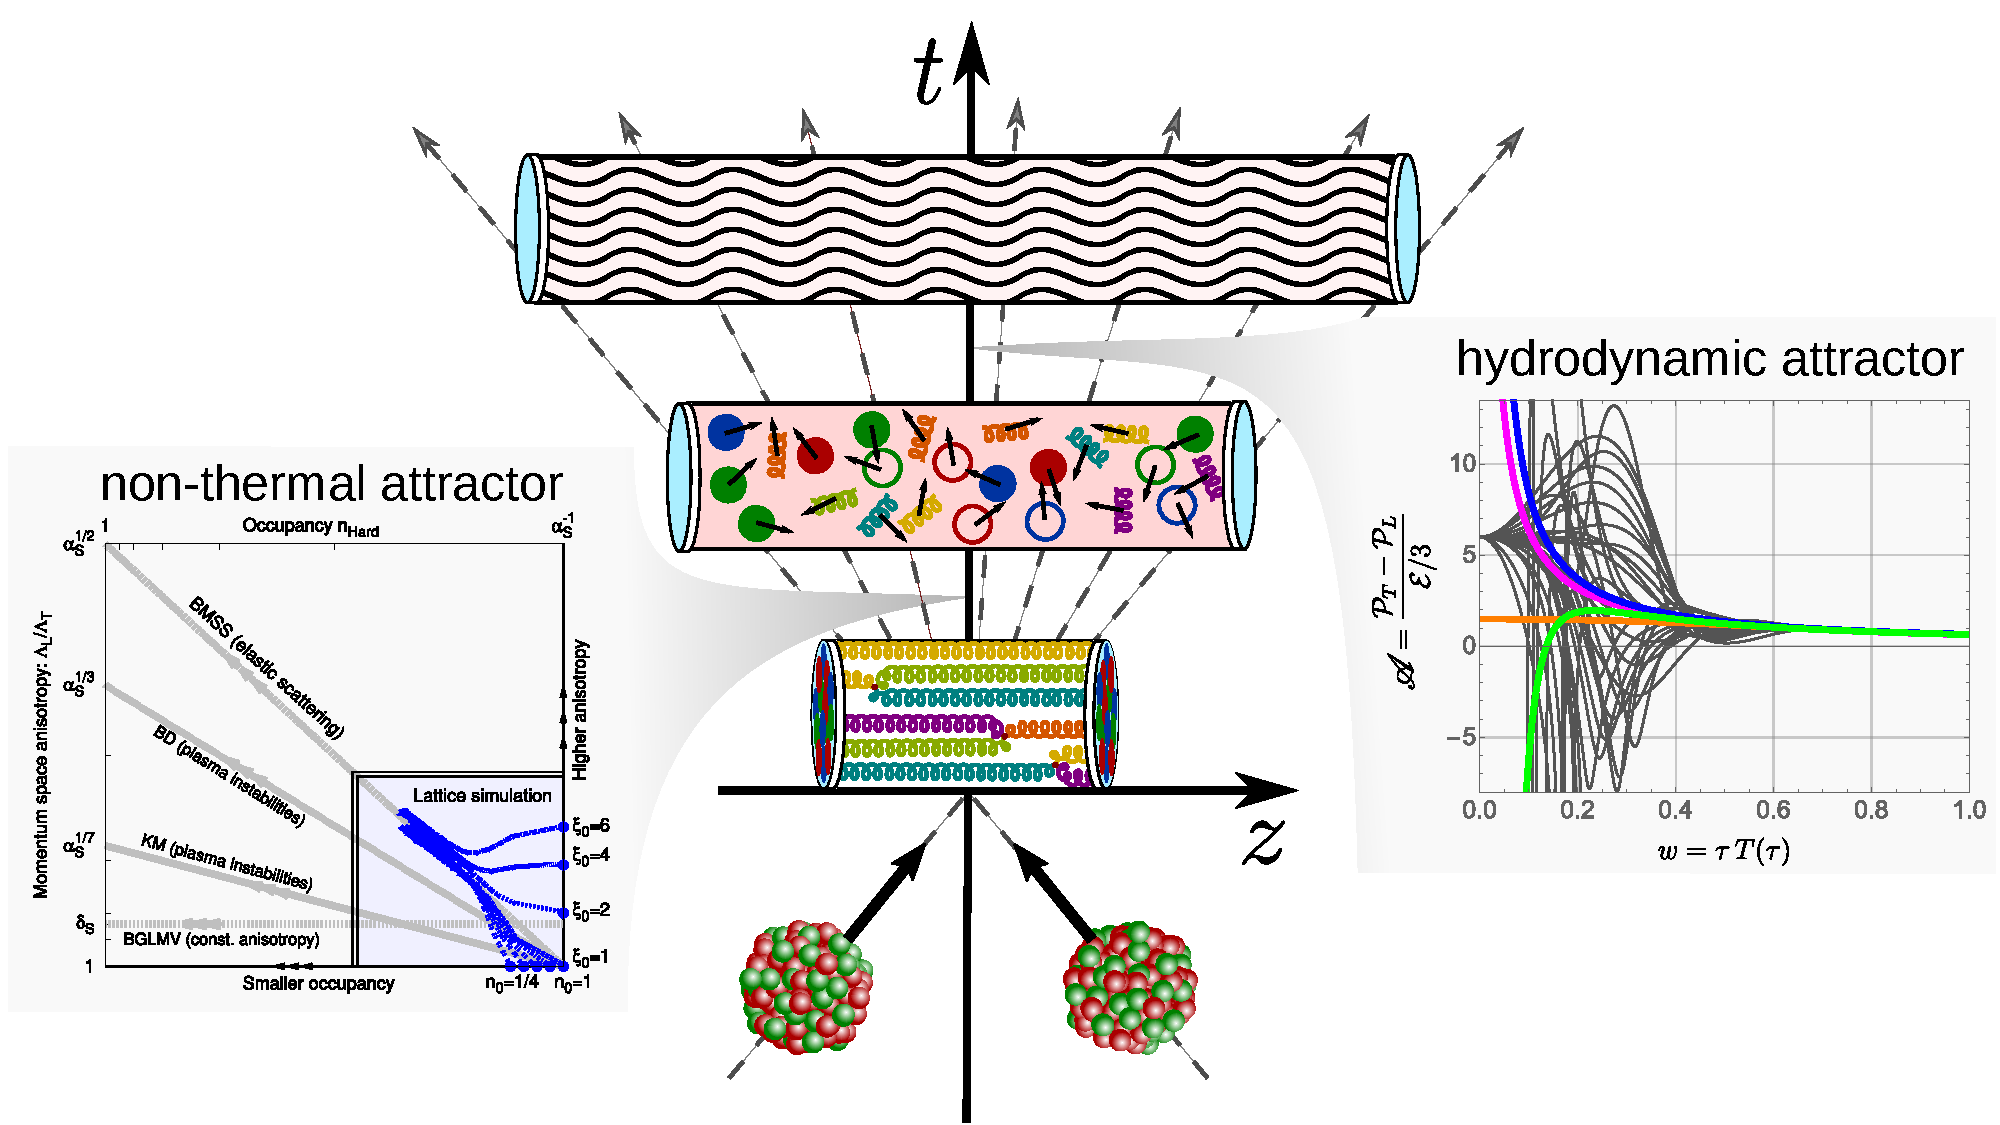
\includegraphics[height=0.7\paperheight]{images/fig01_cover_figure_RB10070_Berges.pdf}} 
    \\[10pt]  
   };
}
\begin{frame}{Brief outline}
    \begin{center}
        \tableofcontents
    \end{center}
\end{frame}
\setbeamertemplate{background}{}

%%%%%%%%%%%%%%%%%%%%%%%%%%%%%%%%%%%%%%%%%
%%%%%%%%%%%%%%%%% SLIDE %%%%%%%%%%%%%%%%%
%%%%%%%%%%%%%%%%%%%%%%%%%%%%%%%%%%%%%%%%%

\setbeamertemplate{background}{
\tikz[overlay,remember picture] \node[at=(current page.center), align=center] {
    \\[15pt]
    {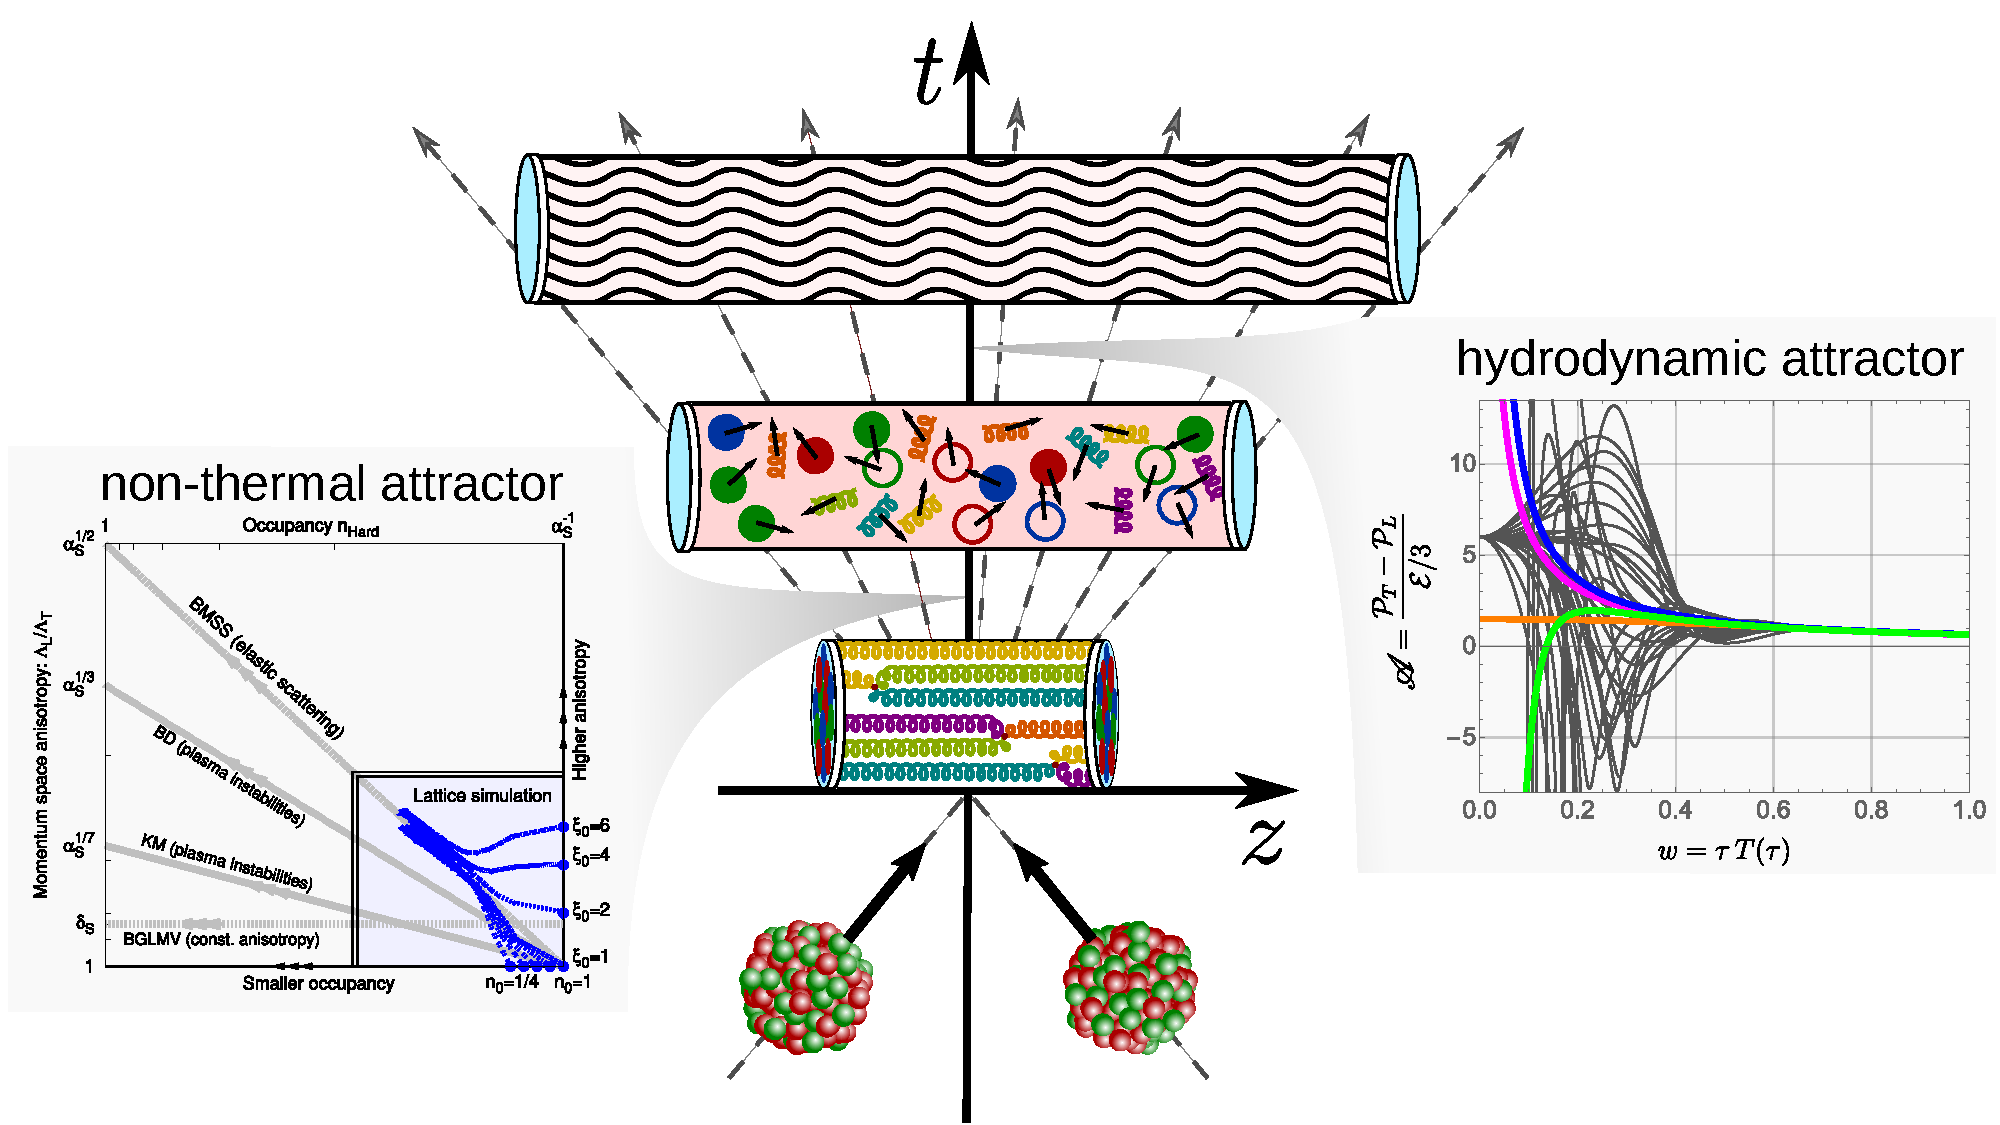
\includegraphics[height=0.7\paperheight]{images/fig01_cover_figure_RB10070_Berges.pdf}} 
    \\[10pt]  
   };
}
\begin{frame}[noframenumbering]
    \frametitle{{\color{jyured}Pre-equilibrium} dynamics}
    \blfootnote{\scriptsize Berges, Heller, Mazeliauskas, Venugopalan \href{https://arxiv.org/abs/2005.12299}{{\color{customblue}\texttt{[2005.12299]}}}}
\end{frame}
\setbeamertemplate{background}{}


\setcounter{framenumber}{0}
\setbeamertemplate{footline}[progress bar]
\setbeamercolor{progress bar}{fg=customblue,bg=fondo}
\addtobeamertemplate{headline}{}{\vspace{1cm}\hfill\circcounter\hspace*{1cm}}
\addtobeamertemplate{frametitle}{\vspace{-0.8cm}}{}

%%%%%%%%%%%%%%%%%%%%%%%%%%%%%%%%%%%%%%%%%
%%%%%%%%%%%%%%%% SECTION %%%%%%%%%%%%%%%%
%%%%%%%%%%%%%%%%%%%%%%%%%%%%%%%%%%%%%%%%%

\section{General context}

%%%%%%%%%%%%%%%%%%%%%%%%%%%%%%%%%%%%%%%%%
%%%%%%%%%%%%%%%%% SLIDE %%%%%%%%%%%%%%%%%
%%%%%%%%%%%%%%%%%%%%%%%%%%%%%%%%%%%%%%%%%

\begin{frame}
    \frametitle{High-energy collisions}
    \framesubtitle{Stitching together effective theories}

    \begin{center}
        \begin{tikzpicture}
            \node[anchor=south west,inner sep=0] at (0,0) {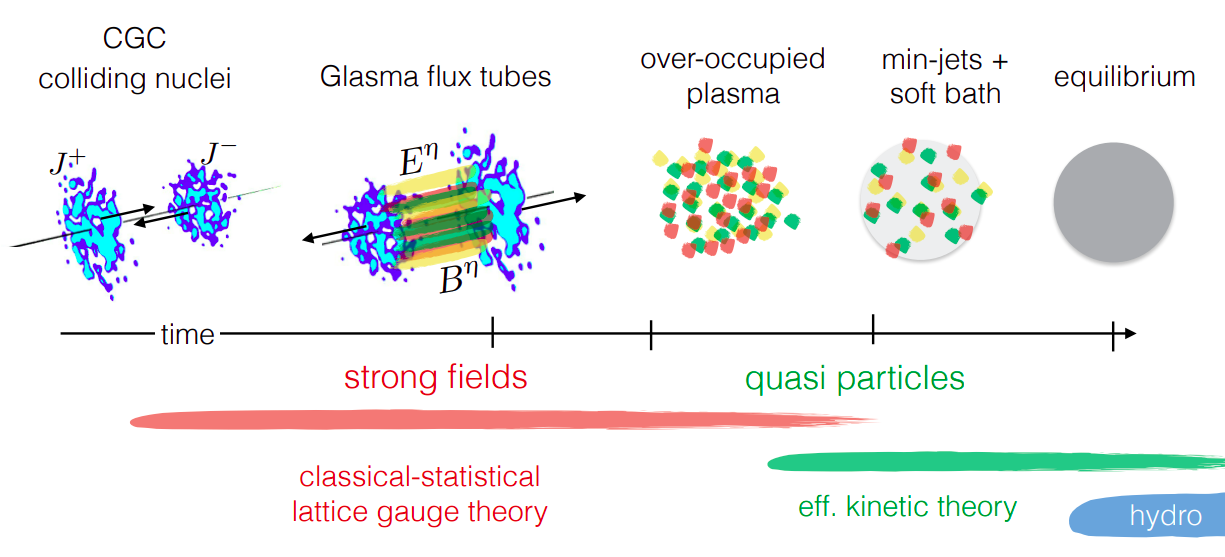
\includegraphics[width=0.8\textwidth]{images/schlichting_initial_stages_2016.png}};
        \end{tikzpicture}
    \end{center}
        
    \blfootnote{\scriptsize Schlichting \href{https://indico.cern.ch/event/469857/contributions/1978347/attachments/1277798/1896654/SchlichtingIS2016.pdf}{{\color{customblue}\texttt{[Initial Stages (2016)]}}}}
\end{frame}

%%%%%%%%%%%%%%%%%%%%%%%%%%%%%%%%%%%%%%%%%
%%%%%%%%%%%%%%%%% SLIDE %%%%%%%%%%%%%%%%%
%%%%%%%%%%%%%%%%%%%%%%%%%%%%%%%%%%%%%%%%%

\setbeamertemplate{itemize item}{\raisebox{0.2em}{\scalebox{0.7}{${\color{pinky}\blacktriangleright}$}}} 

\begin{frame}[noframenumbering]
    \frametitle{High-energy collisions}
    \framesubtitle{{\color{jyured}Pre-equilibrium} stages}
    
    \begin{center}
        \begin{tikzpicture}[]
            \node[anchor=south west,inner sep=0] at (0,0) {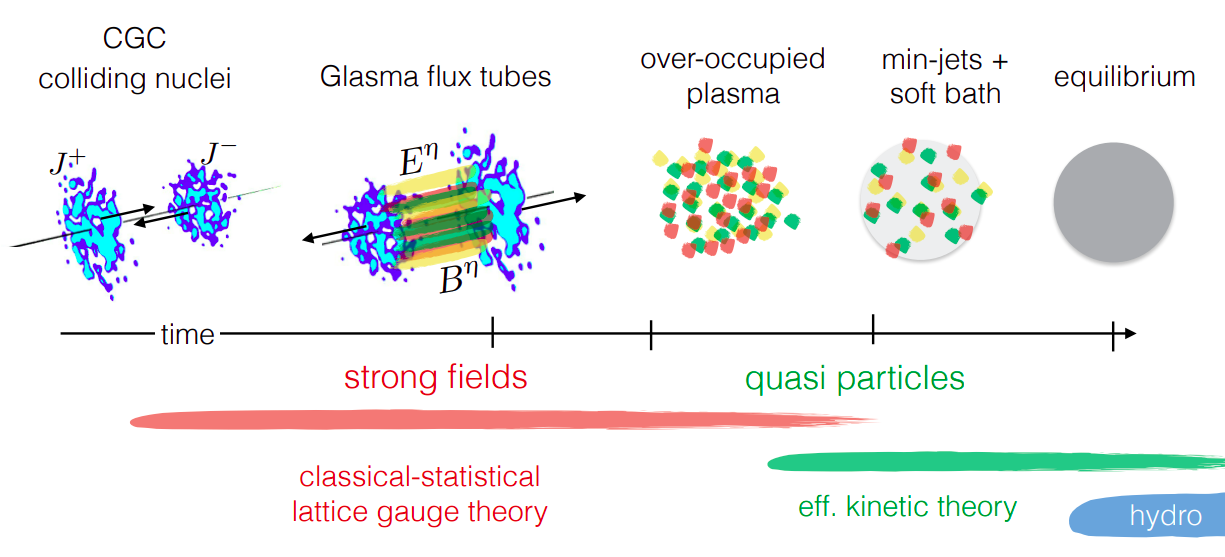
\includegraphics[width=0.8\textwidth]{images/schlichting_initial_stages_2016.png}};
            \draw<1>[white, fill=white, fill opacity=0.9] (8.37,0) rectangle (\textheight+4.6cm,5.5) node[pos=0.5, anchor=center, xshift=0.03\linewidth,text width=4cm] {{\Large\color{pinky} Glasma stage\footnotemark}\\[10pt]\footnotesize\begin{itemize}
                \item Gluons as color fields
                \item Classical gauge fields
                \item Weak coupling regime
                \item Color Glass Condensate
                \item Real-time classical lattice gauge theory
            \end{itemize}
            };
            \draw<1>[pinky,thick,fill=pinky,fill opacity=0.1] (0,0) rectangle (\textheight+0.6cm,5.5);
        \end{tikzpicture}
    \end{center}
        
    \footnotetext{\scriptsize Gelis \href{https://doi.org/10.1142/S0217751X13300019}{{\color{customblue}\texttt{[Int.J.Mod.Phys.A28(2013)]}}}}
    \blfootnote{\scriptsize Schlichting \href{https://indico.cern.ch/event/469857/contributions/1978347/attachments/1277798/1896654/SchlichtingIS2016.pdf}{{\color{customblue}\texttt{[Initial Stages (2016)]}}}}
\end{frame}

%%%%%%%%%%%%%%%%%%%%%%%%%%%%%%%%%%%%%%%%%
%%%%%%%%%%%%%%%%% SLIDE %%%%%%%%%%%%%%%%%
%%%%%%%%%%%%%%%%%%%%%%%%%%%%%%%%%%%%%%%%%

\setbeamertemplate{itemize item}{\raisebox{0.2em}{\scalebox{0.7}{${\color{ming}\blacktriangleright}$}}} 

\begin{frame}[noframenumbering]
    \frametitle{High-energy collisions}
    \framesubtitle{{\color{jyured}Pre-equilibrium} stages}
    
    \begin{center}
        \begin{tikzpicture}[]
            \node[anchor=south west,inner sep=0] at (0,0) {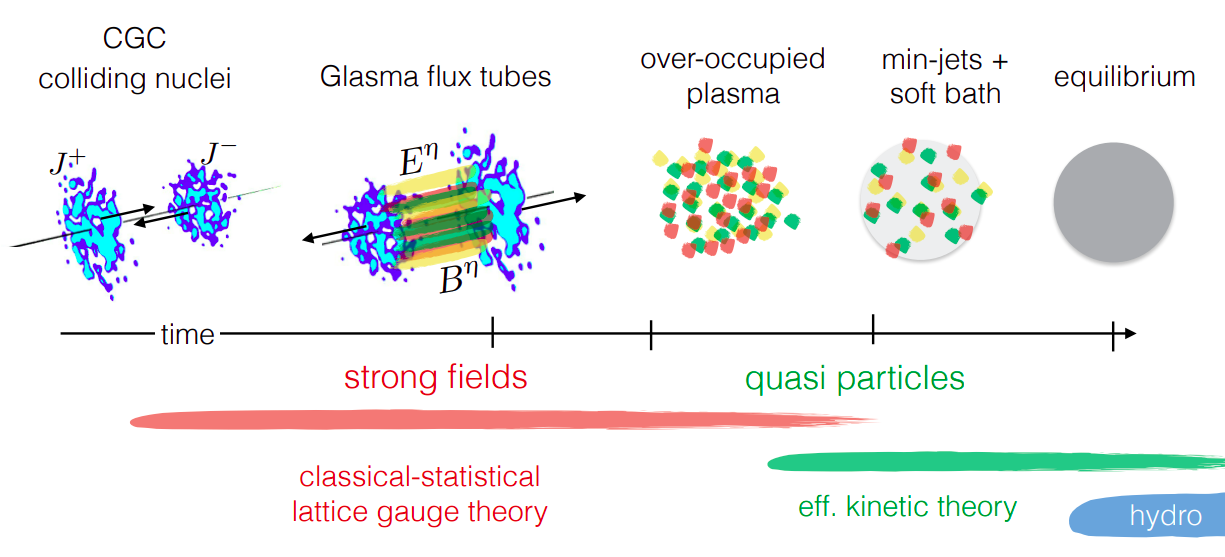
\includegraphics[width=0.8\textwidth]{images/schlichting_initial_stages_2016.png}};
            \draw<1>[white, fill=white, fill opacity=0.9] (0,0) rectangle (\textheight-1.55cm,5.5) node[pos=0.5, anchor=center, xshift=-0.01\linewidth,text width=5.5cm] {{\Large\color{ming} Kinetic theory\footnotemark}\\[10pt]\footnotesize\begin{itemize}
                \item Gluons as quasi-particles
                \item Distribution functions
                \item Weak coupling regime
                \item Bottom-up thermalization 
                \item AMY effective kinetic theory 
            \end{itemize}
            };
            \draw<1>[ming,thick,fill=ming,fill opacity=0.1] (6.2,0) rectangle (\textheight+4.6cm,5.5);
        \end{tikzpicture}
    \end{center}
        
    \footnotetext{\scriptsize Kurkela, Mazeliauskas, Paquet, Schlichting, Teaney \href{https://journals.aps.org/prc/abstract/10.1103/PhysRevC.99.034910}{{\color{customblue}\texttt{[Phys.Rev.C99(2019)]}}}}
    \blfootnote{\scriptsize Schlichting \href{https://indico.cern.ch/event/469857/contributions/1978347/attachments/1277798/1896654/SchlichtingIS2016.pdf}{{\color{customblue}\texttt{[Initial Stages (2016)]}}}}
\end{frame}

%%%%%%%%%%%%%%%%%%%%%%%%%%%%%%%%%%%%%%%%%
%%%%%%%%%%%%%%%% SECTION %%%%%%%%%%%%%%%%
%%%%%%%%%%%%%%%%%%%%%%%%%%%%%%%%%%%%%%%%%

\section{{\color{jyured}Pre-equilibrium} dynamics}

%%%%%%%%%%%%%%%%%%%%%%%%%%%%%%%%%%%%%%%%%%%%
%%%%%%%%%%%%%%%% SUBSECTION %%%%%%%%%%%%%%%%
%%%%%%%%%%%%%%%%%%%%%%%%%%%%%%%%%%%%%%%%%%%%

\subsection{Glasma}

%%%%%%%%%%%%%%%%%%%%%%%%%%%%%%%%%%%%%%%%%
%%%%%%%%%%%%%%%%% SLIDE %%%%%%%%%%%%%%%%%
%%%%%%%%%%%%%%%%%%%%%%%%%%%%%%%%%%%%%%%%%

\setbeamertemplate{background}{
\tikz[overlay,remember picture] \node[opacity=0.1, at=(current page.center), align=center] {\\[10pt]
{\transparent{0.2}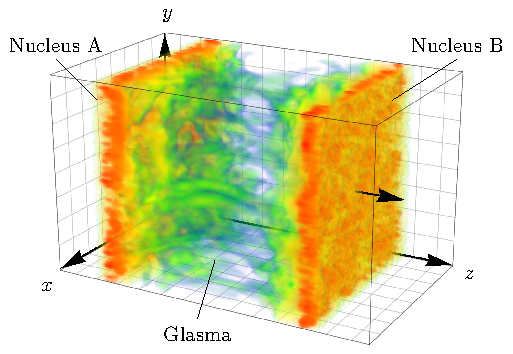
\includegraphics[height=0.8\paperheight]{images/fig1_overview.pdf}}};
}
\begin{frame}[plain,noframenumbering]{}
    \begin{center}
        \vspace{1cm}
        {\large\color{normal}Initial stage of pre-equilibrium}\\[0.3cm]
        {\huge\color{destacado}The glasma}
    \end{center}
\end{frame}
\setbeamertemplate{background}{}

%%%%%%%%%%%%%%%%%%%%%%%%%%%%%%%%%%%%%%%%%
%%%%%%%%%%%%%%%%% SLIDE %%%%%%%%%%%%%%%%%
%%%%%%%%%%%%%%%%%%%%%%%%%%%%%%%%%%%%%%%%%

\setbeamertemplate{background}{
\tikz[overlay,remember picture] \node[at=(current page.center), align=center] {\\[10pt]
{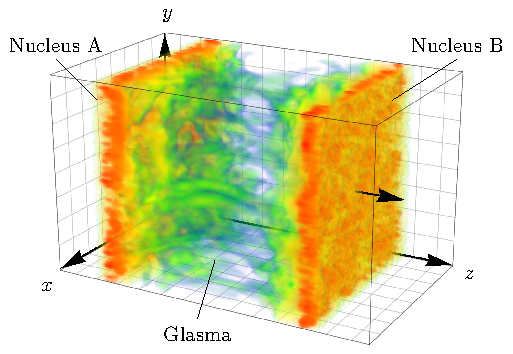
\includegraphics[height=0.8\paperheight]{images/fig1_overview.pdf}}};
}
\begin{frame}[plain,noframenumbering]{}
    \blfootnote{\scriptsize Ipp, Müller  \href{https://doi.org/10.1016/j.physletb.2017.05.032}{{\color{customblue}\texttt{[Phys.Lett.B771(2017)]}}}}
\end{frame}
\setbeamertemplate{background}{}

%%%%%%%%%%%%%%%%%%%%%%%%%%%%%%%%%%%%%%%%%
%%%%%%%%%%%%%%%%% SLIDE %%%%%%%%%%%%%%%%%
%%%%%%%%%%%%%%%%%%%%%%%%%%%%%%%%%%%%%%%%%

\begin{frame}
    \frametitle{Color Glass Condensate}
    \framesubtitle{An EFT for high energy QCD}
    \vspace{-10pt}
    \begin{columns}[onlytextwidth,t]
        \column{.033\textwidth}
       \column{.5\textwidth}
            \begin{center}
                {\footnotesize Separation of scales between\\
                {\color{customgreen}small-{\tiny $x$}} and {\color{custompink}large-{\huge $x$}} degrees of freedom\footnotemark}
            \end{center}
            \vspace{-10pt}
            \begin{figure}[!hbt]
                \centering
                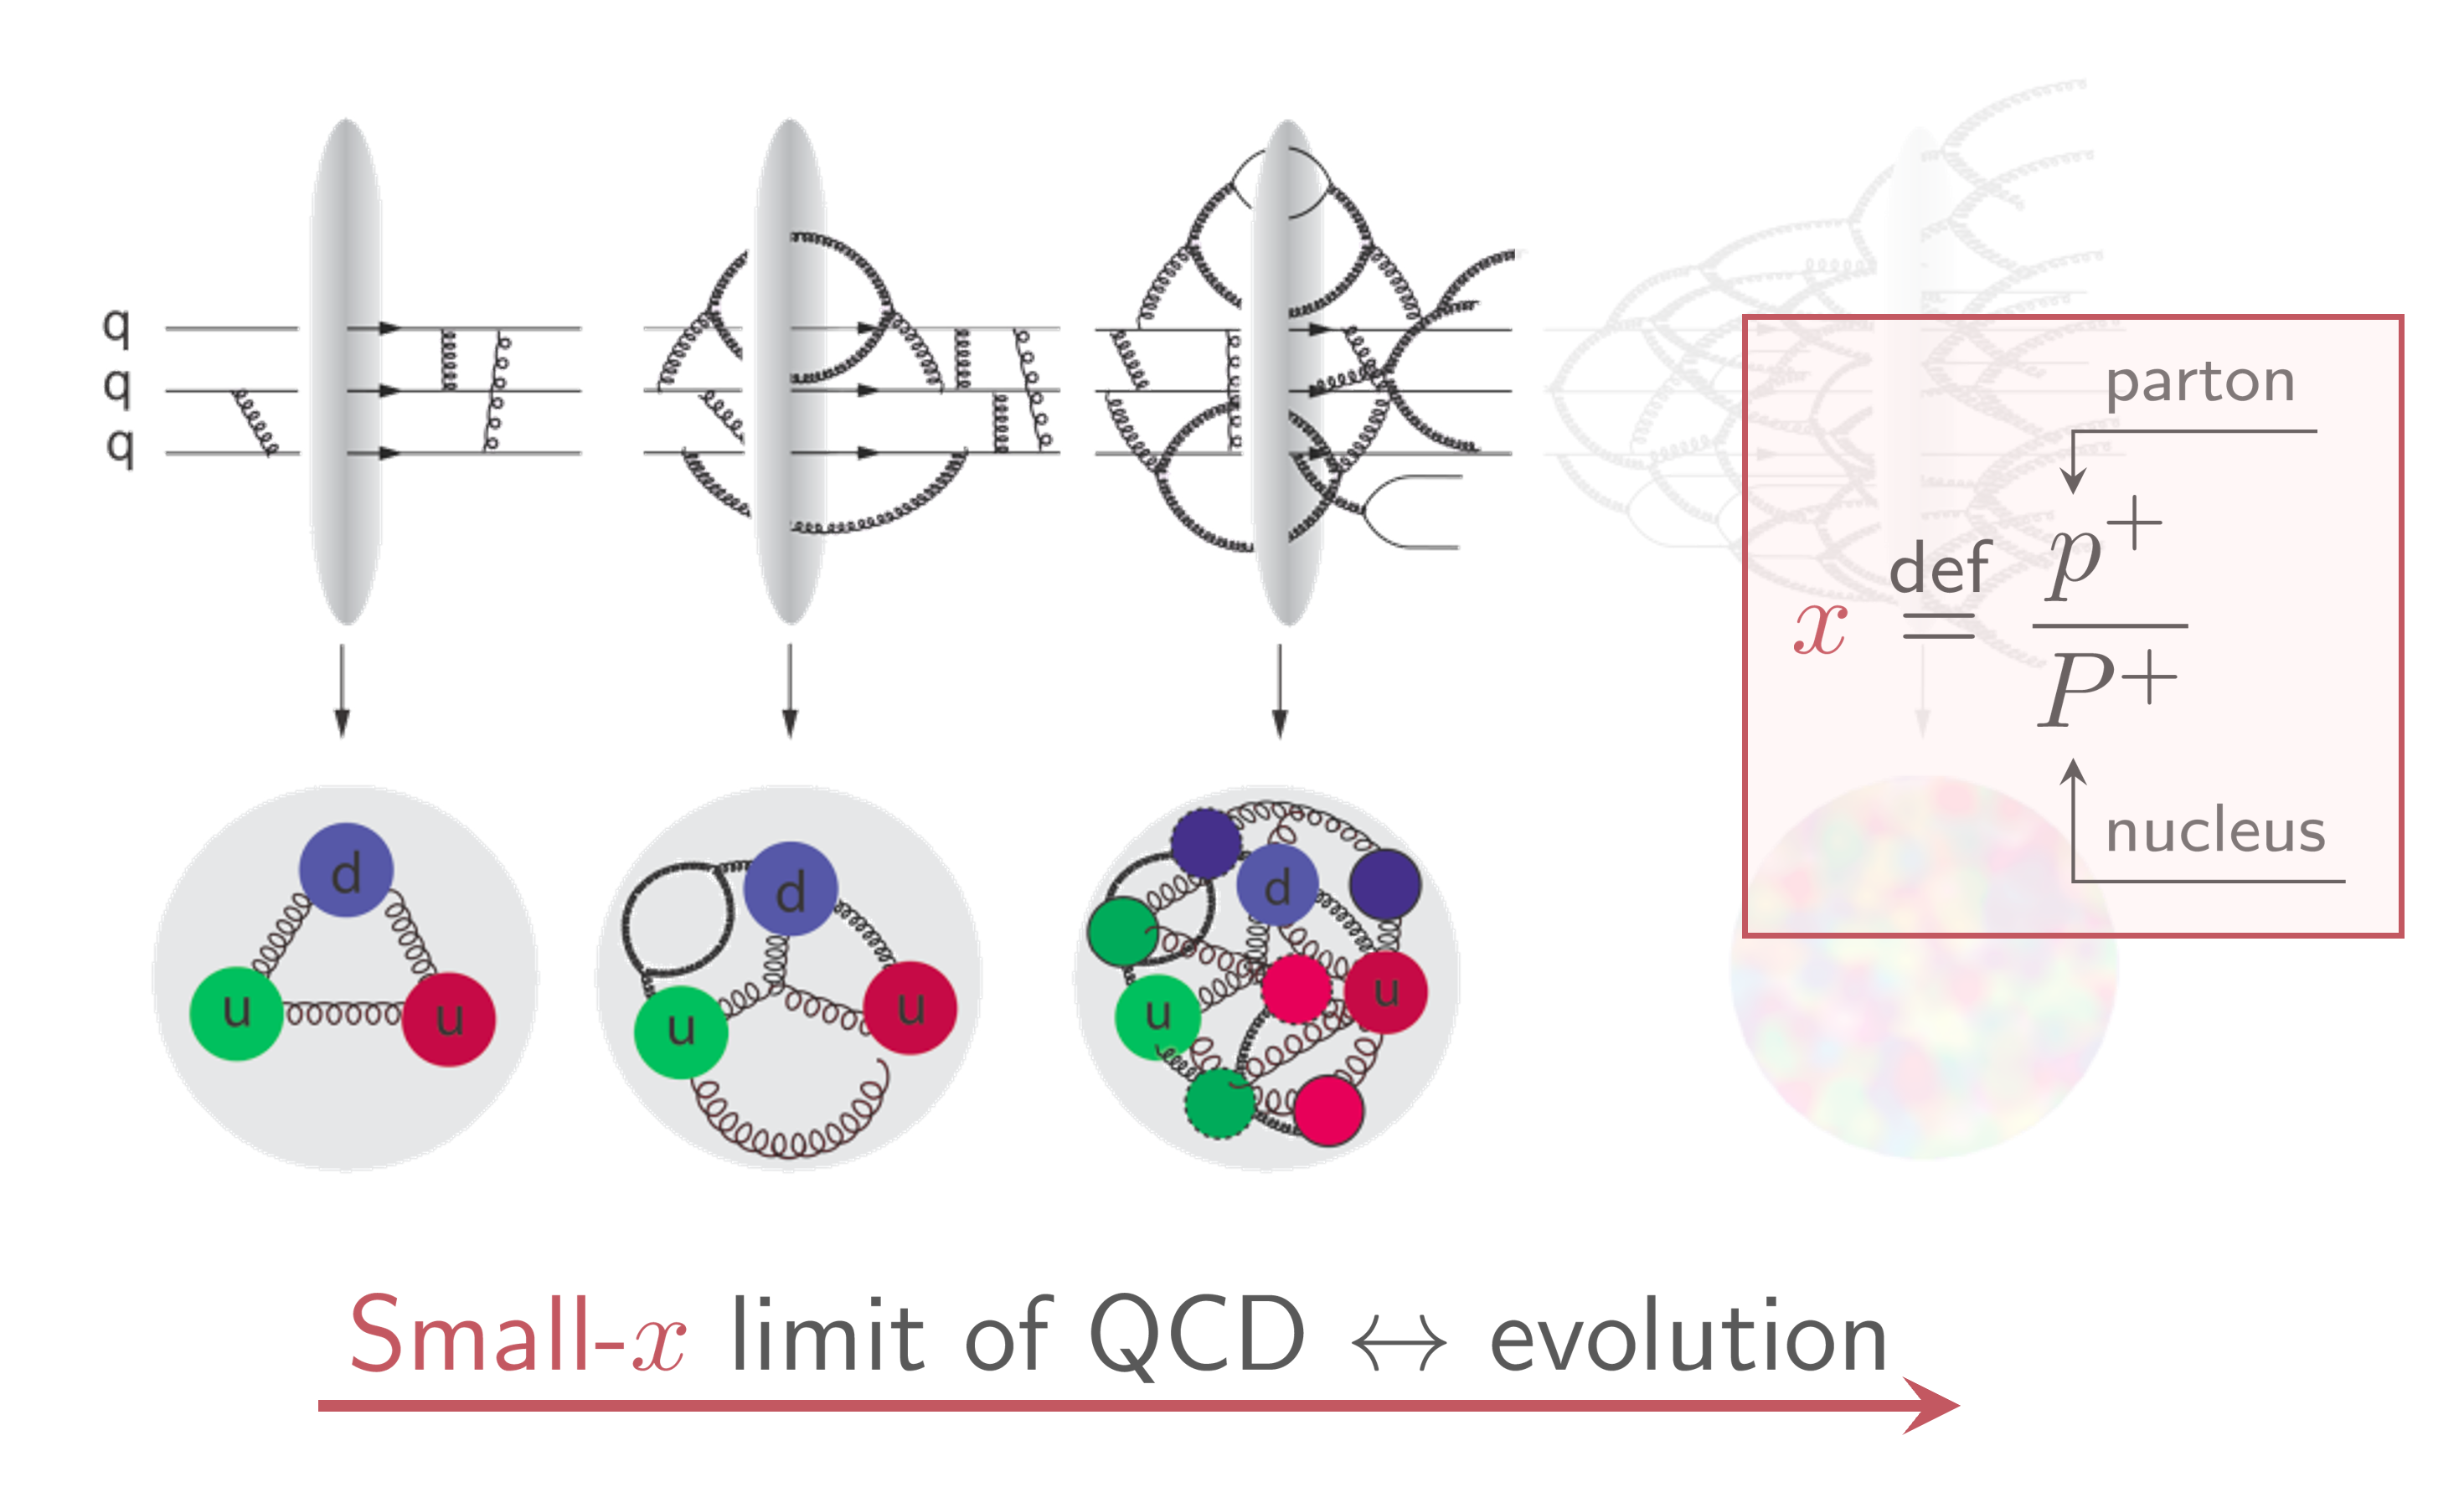
\includegraphics[width=\textwidth]{images/qcd_1.png}
                \captionsetup{justification=centering}
            \end{figure}
        \column{.033\textwidth}
        \column{.4\textwidth}
        \begin{center}
            {\transparent{0.2}
            \begin{figure}[!hbt]
                \centering
                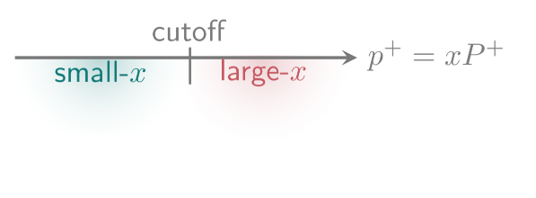
\includegraphics[width=0.9\textwidth]{images/small_large_x.png}
                \captionsetup{justification=centering}
                \vspace{-0.2em}
            \end{figure}
            \footnotesize
            \vspace{-10pt}
            Classical Yang-Mills equations\\[20pt]
            \renewcommand{\eqnhighlightheight}{\vphantom{\mathcal{D}_\mu}\mathstrut}\begin{equation*}
                \Big(\eqnmark[starrymain]{dmu}{\mathcal{D}_\mu}\eqnmark[starrysecond]{fmunu}{F^{\mu\nu}}\Big)\Big[\eqnmark[customgreen]{amu}{A^\mu}\Big]=\eqnmark[custompink]{jnu}{J^\nu}
                \end{equation*}
                \annotate[yshift=2.2em]{above, right}{dmu}{\scriptsize covariant derivative}
                \annotate[yshift=0.7em]{above}{fmunu}{\scriptsize field strength tensor}
                \annotate[yshift=-0.5em]{below, left}{amu}{\scriptsize gluons gauge field}
                \annotate[yshift=-2em]{below, left}{jnu}{\scriptsize color current of nucleus}}
        \end{center}
        \column{.033\textwidth}
    \end{columns}
    \footnotetext{\scriptsize Gelis, Iancu, Jalilian-Marian, Venugopalan \href{https://doi.org/10.1146/annurev.nucl.010909.083629}{{\color{customblue}\texttt{[Ann.Rev.Nucl.Part.Sci.60(2010)]}}}}
    \blfootnote{\scriptsize Artwork by T. Ullrich}
\end{frame}


%%%%%%%%%%%%%%%%%%%%%%%%%%%%%%%%%%%%%%%%%
%%%%%%%%%%%%%%%%% SLIDE %%%%%%%%%%%%%%%%%
%%%%%%%%%%%%%%%%%%%%%%%%%%%%%%%%%%%%%%%%%

\begin{frame}[noframenumbering]
    \frametitle{Color Glass Condensate}
    \framesubtitle{An EFT for high energy QCD}
    \vspace{-10pt}
    \begin{columns}[onlytextwidth,t]
        \column{.033\textwidth}
       \column{.5\textwidth}
            \begin{center}
                {\footnotesize Separation of scales between\\
                {\color{customgreen}small-{\tiny $x$}} and {\color{custompink}large-{\huge $x$}} degrees of freedom}
            \end{center}
            \vspace{-10pt}
            \begin{figure}[!hbt]
                \centering
                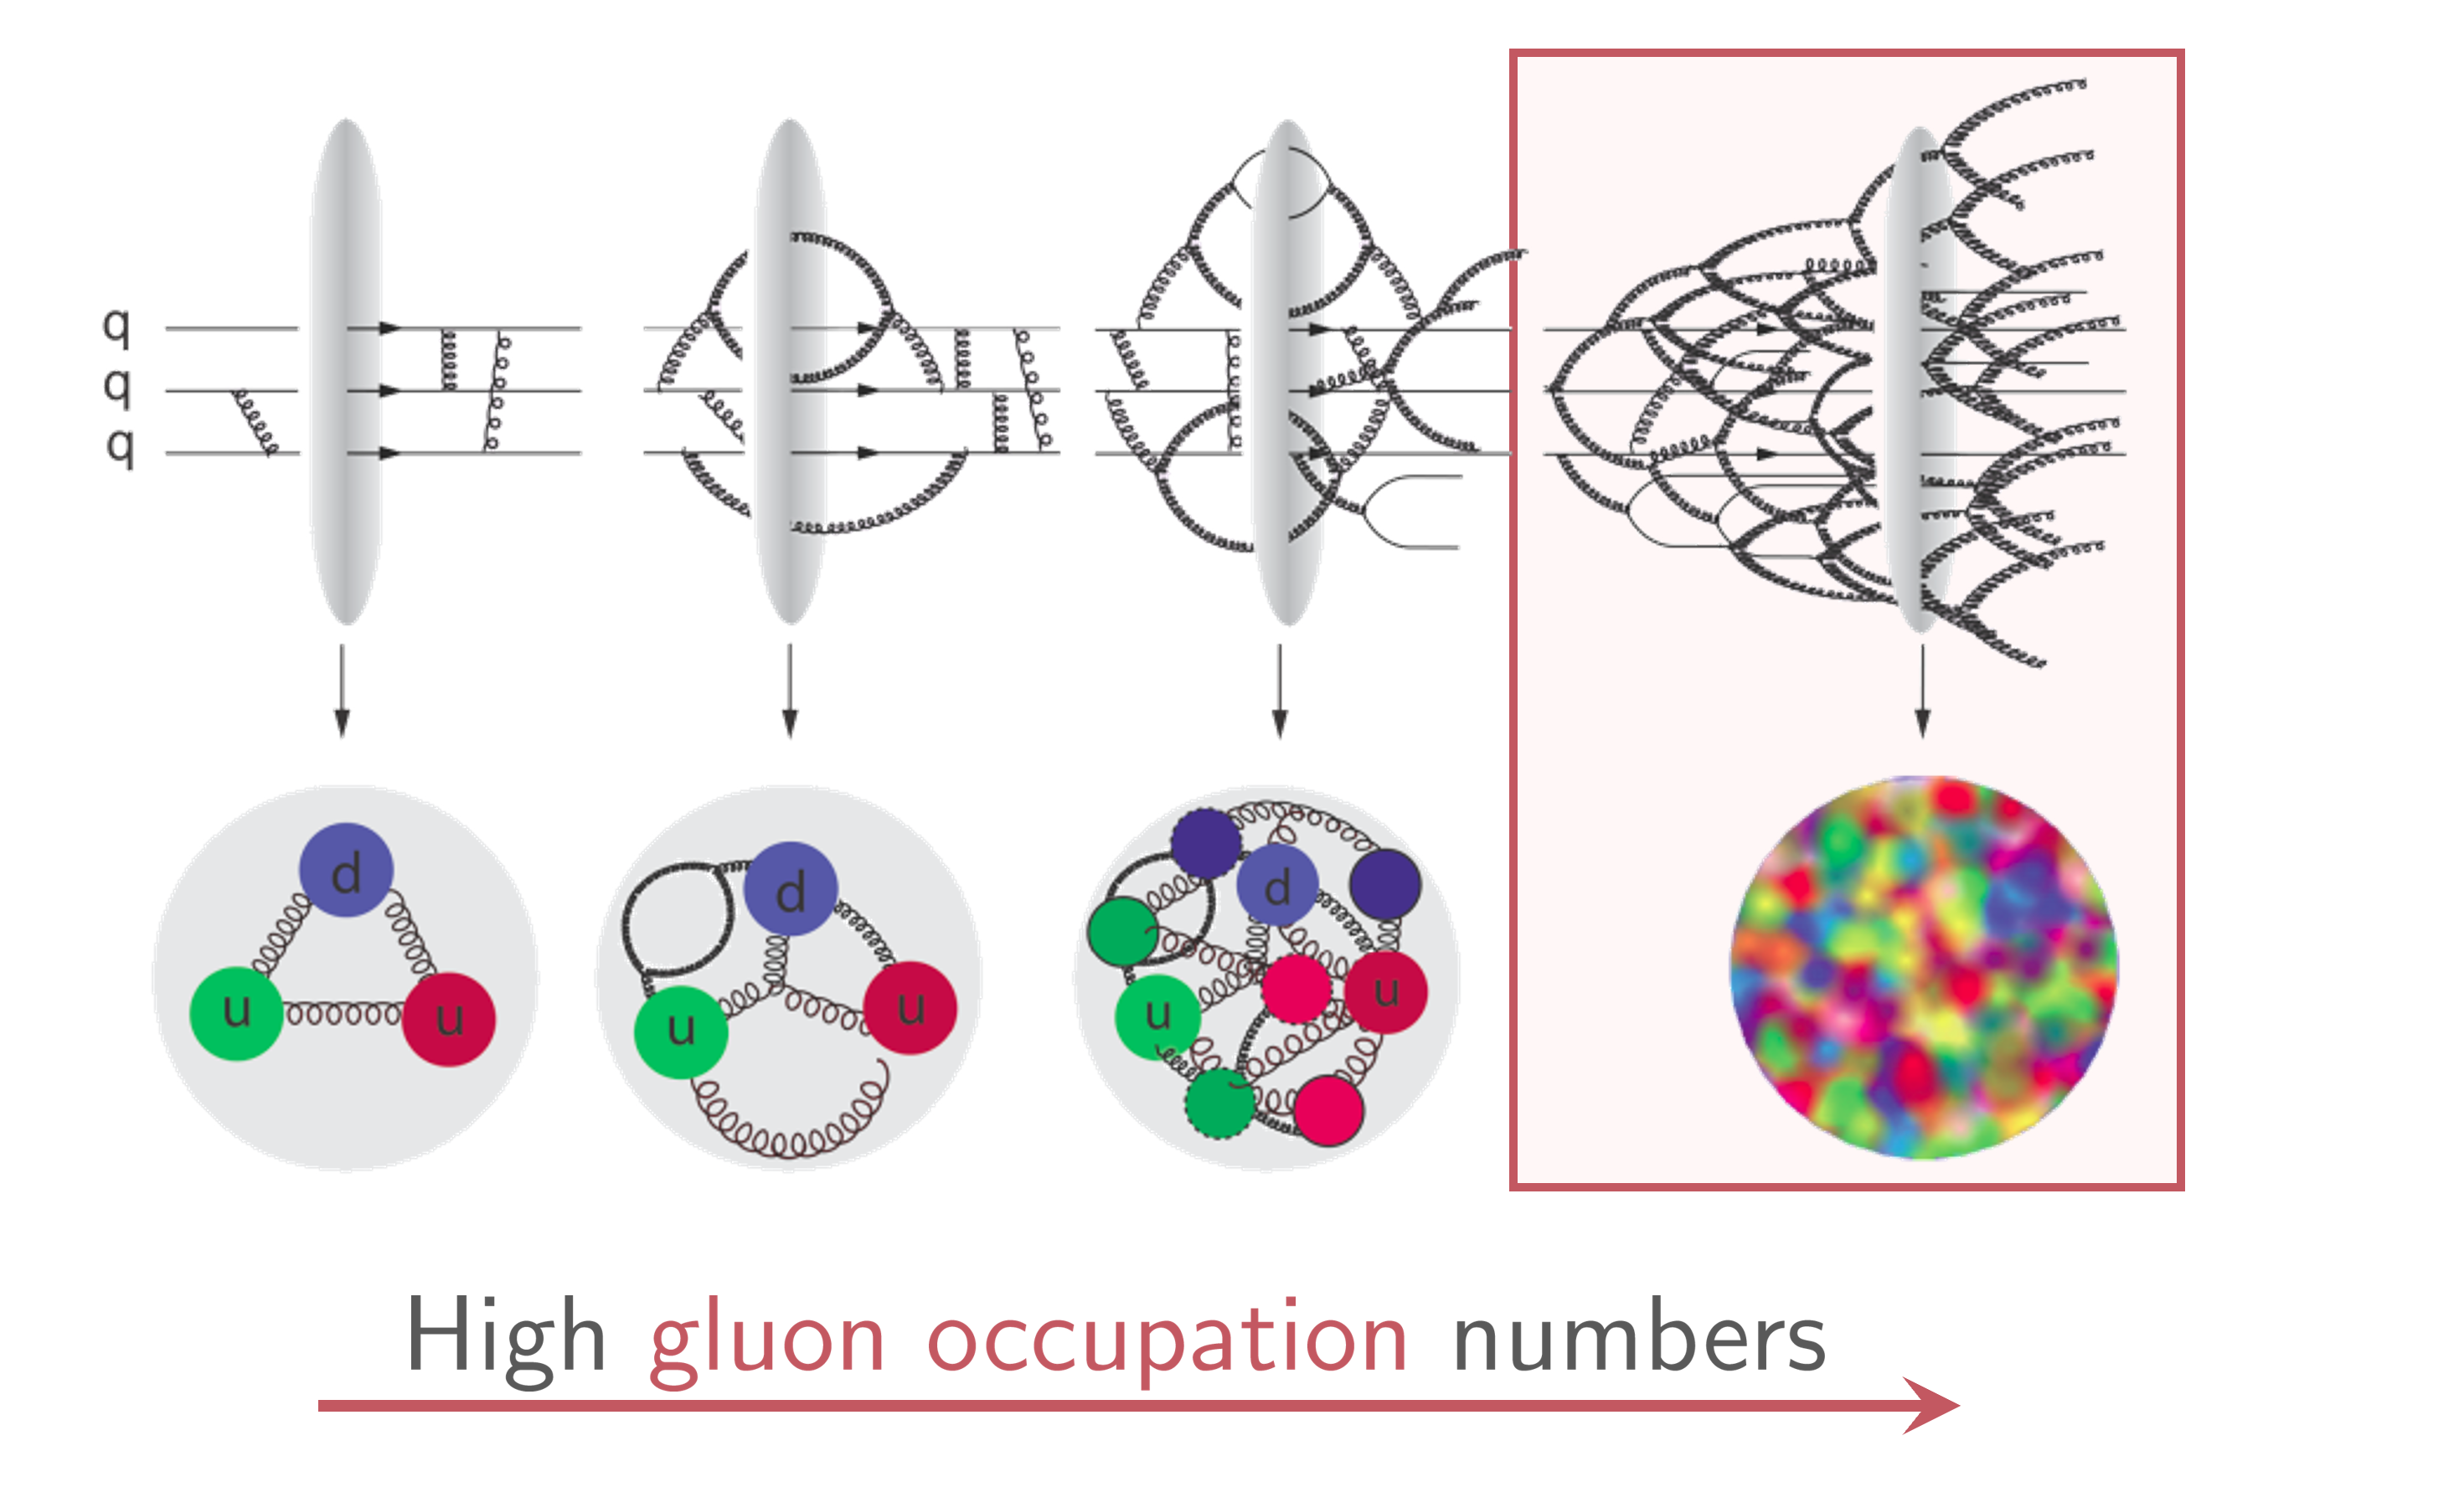
\includegraphics[width=\textwidth]{images/qcd_2.png}
                \captionsetup{justification=centering}
            \end{figure}
        \column{.033\textwidth}
        \column{.4\textwidth}
        \begin{center}
            \begin{figure}[!hbt]
                \centering
                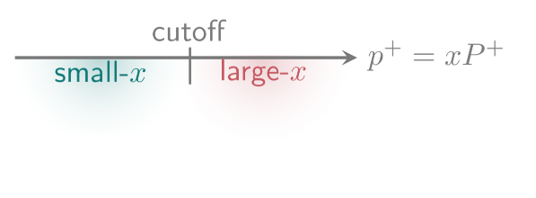
\includegraphics[width=0.9\textwidth]{images/small_large_x.png}
                \captionsetup{justification=centering}
                \vspace{-0.2em}
            \end{figure}
            \footnotesize
            \vspace{-10pt}
            Classical Yang-Mills equations\\[20pt]
            \renewcommand{\eqnhighlightheight}{\vphantom{\mathcal{D}_\mu}\mathstrut}\begin{equation*}
                \Big(\eqnmark[starrymain]{dmu}{\mathcal{D}_\mu}\eqnmark[starrysecond]{fmunu}{F^{\mu\nu}}\Big)\Big[\eqnmark[customgreen]{amu}{A^\mu}\Big]=\eqnmark[custompink]{jnu}{J^\nu}
                \end{equation*}
                \annotate[yshift=2.2em]{above, right}{dmu}{\scriptsize covariant derivative}
                \annotate[yshift=0.7em]{above}{fmunu}{\scriptsize field strength tensor}
                \annotate[yshift=-0.5em]{below, left}{amu}{\scriptsize gluons gauge field}
                \annotate[yshift=-2em]{below, left}{jnu}{\scriptsize color current of nucleus}
        \end{center}
        \column{.033\textwidth}
    \end{columns}
    \footnotetext{\scriptsize Gelis, Iancu, Jalilian-Marian, Venugopalan \href{https://doi.org/10.1146/annurev.nucl.010909.083629}{{\color{customblue}\texttt{[Ann.Rev.Nucl.Part.Sci.60(2010)]}}}}
    \blfootnote{\scriptsize Artwork by T. Ullrich}
\end{frame}


%%%%%%%%%%%%%%%%%%%%%%%%%%%%%%%%%%%%%%%%%
%%%%%%%%%%%%%%%%% SLIDE %%%%%%%%%%%%%%%%%
%%%%%%%%%%%%%%%%%%%%%%%%%%%%%%%%%%%%%%%%%

\begin{frame}
    \frametitle{CGC fields}
    \framesubtitle{Analytical fields before the collision}
    \begin{figure}[!hbt]
        \centering
    	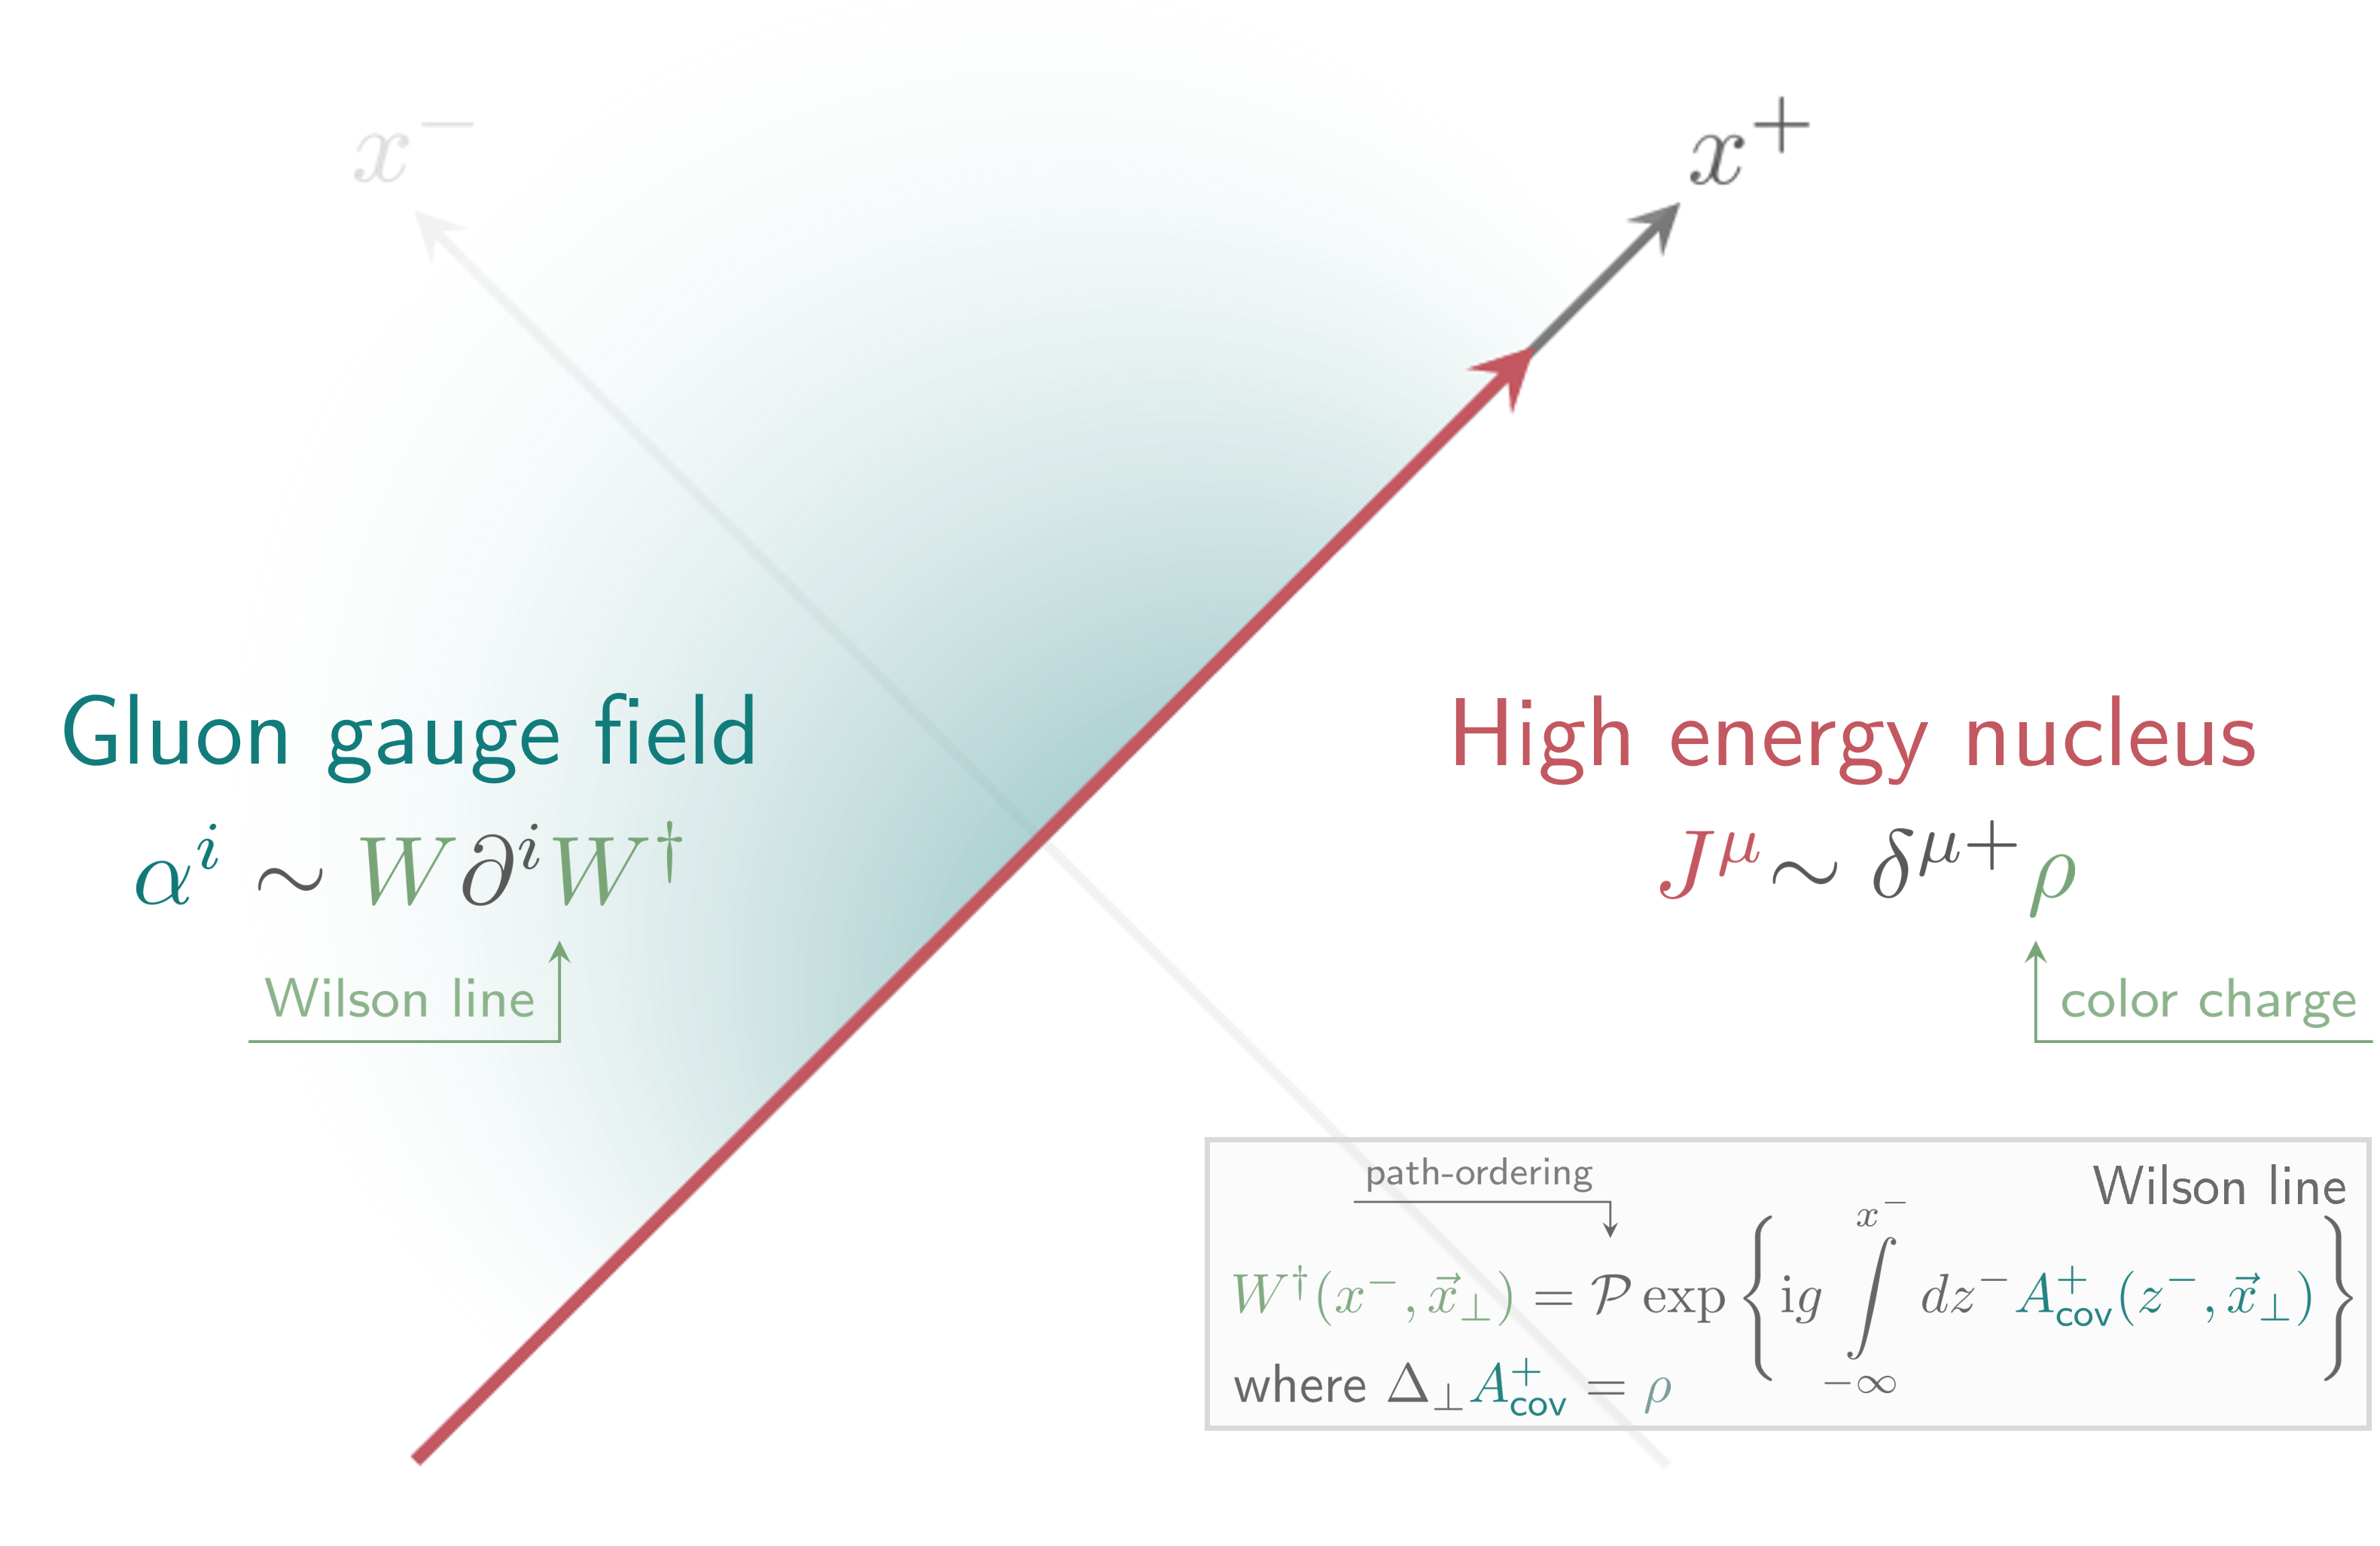
\includegraphics[width=0.7\textwidth]{images/cgc_nuclei.png}
        \captionsetup{justification=centering}
    \end{figure}
\end{frame}

%%%%%%%%%%%%%%%%%%%%%%%%%%%%%%%%%%%%%%%%%
%%%%%%%%%%%%%%%%% SLIDE %%%%%%%%%%%%%%%%%
%%%%%%%%%%%%%%%%%%%%%%%%%%%%%%%%%%%%%%%%%

\begin{frame}[noframenumbering]
    \frametitle{Glasma fields}
    \framesubtitle{Numerical field after the collision}
    \begin{columns}[onlytextwidth,t]
        \column{.02\textwidth}
       \column{.46\textwidth}
       \begin{figure}
            \centering
            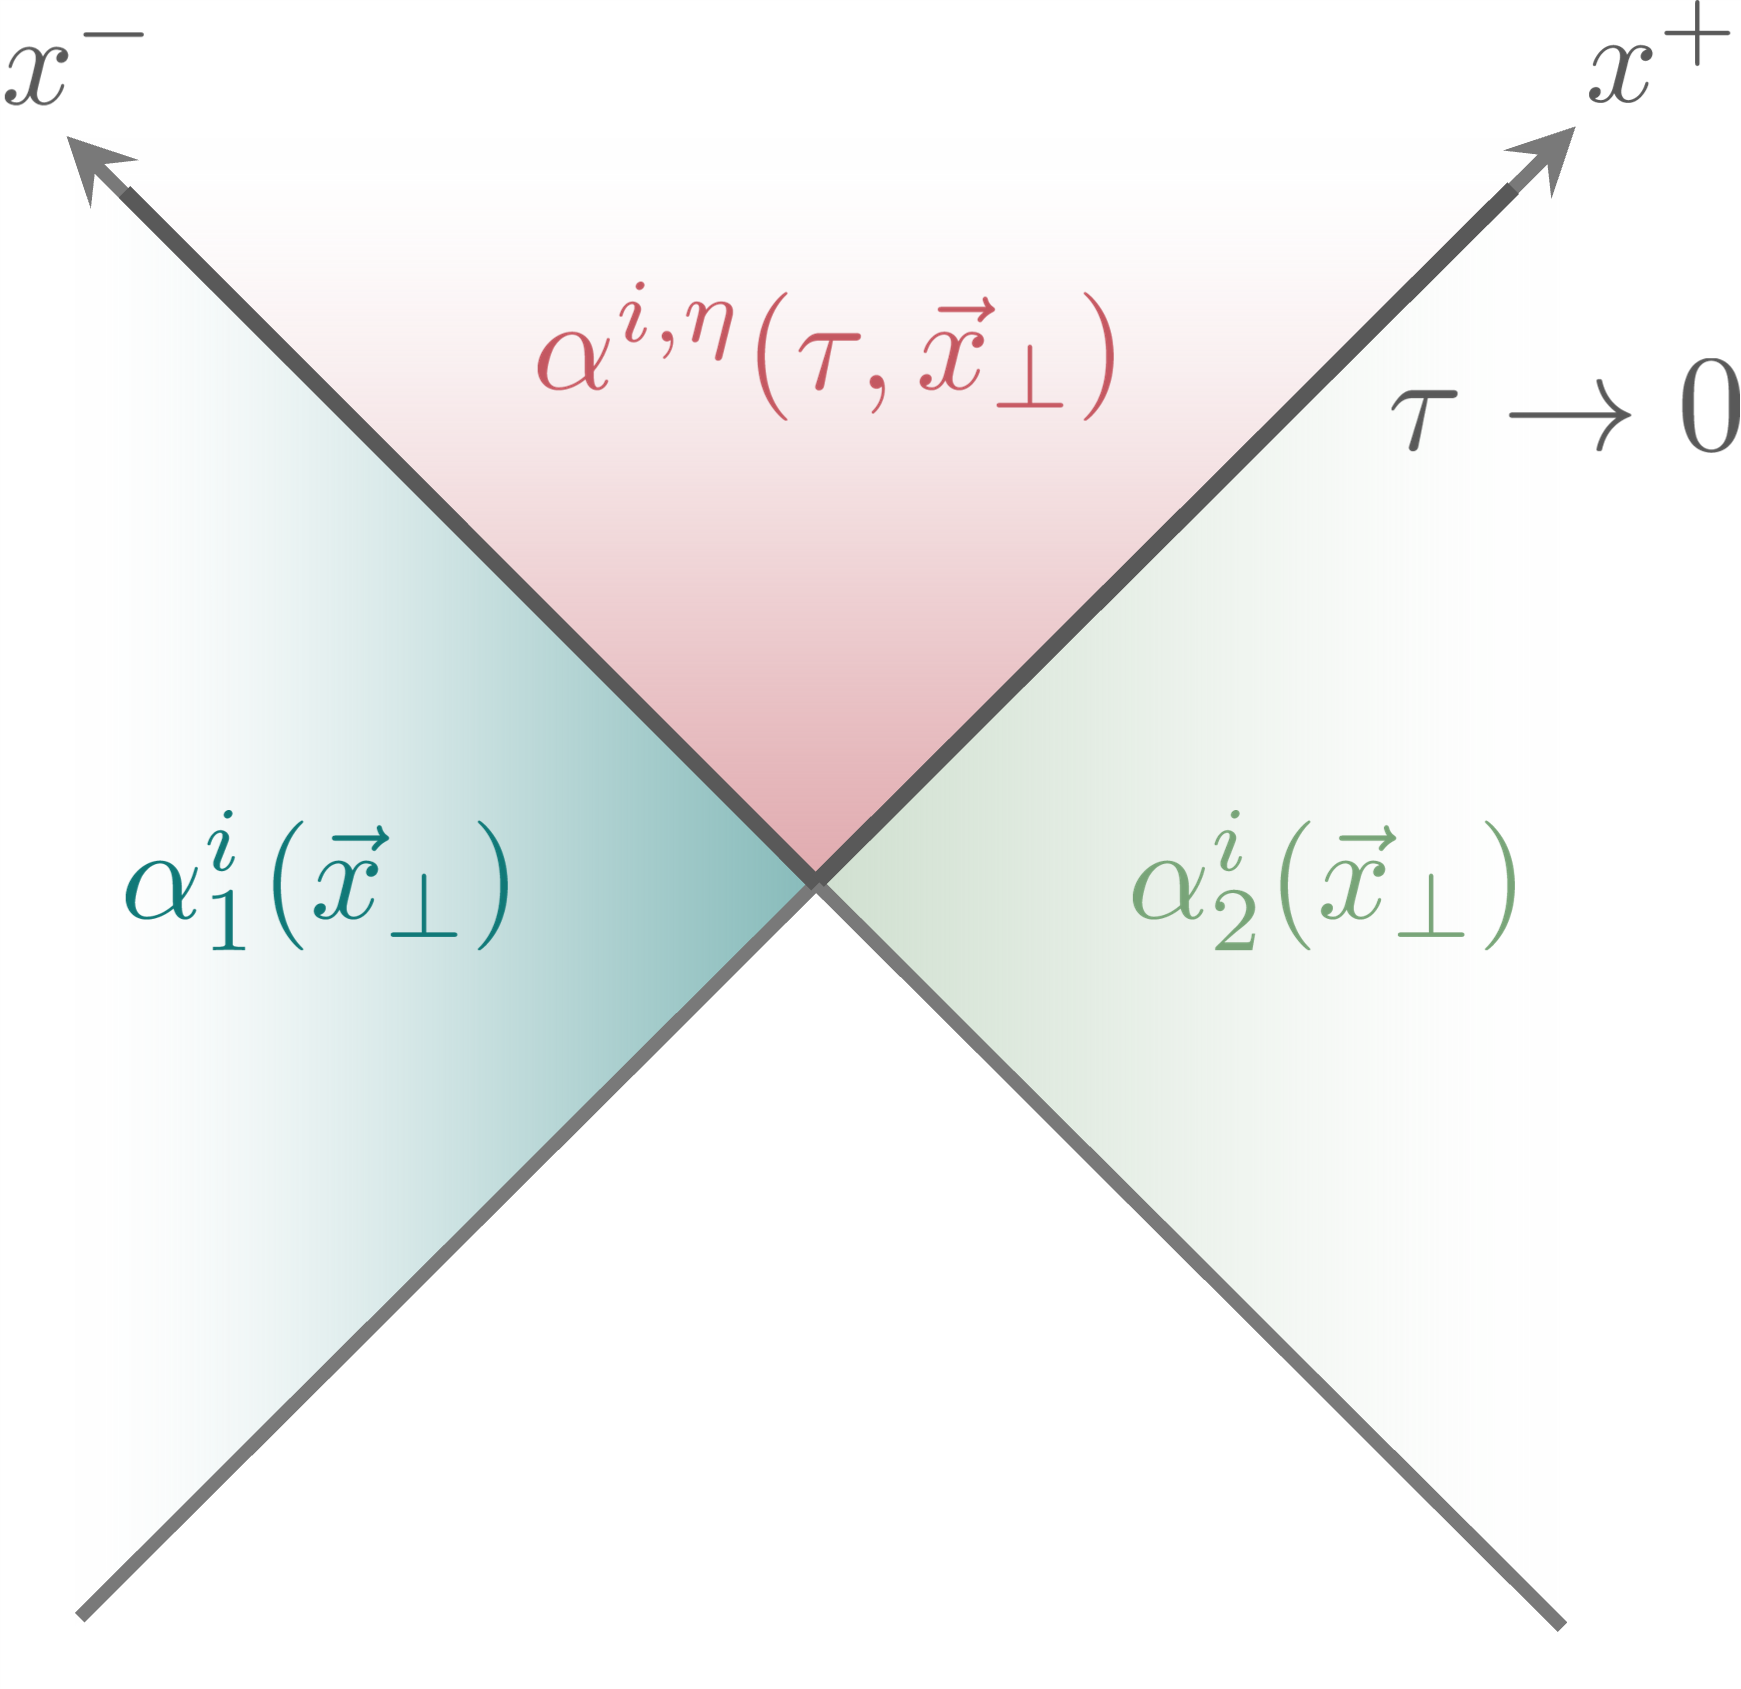
\includegraphics[width=0.85\columnwidth]{images/cgc_col.png}
            \captionsetup{justification=centering}
        \end{figure}
        \column{.02\textwidth}
        \column{.5\textwidth}
        \vspace{0.2cm}
        \begin{center}
            {\color{customgreen}$\sbullet[0.6]$ Known CGC fields} at $\tau<0$ \\[0.1cm]
            {\color{destacado}$\sbullet[0.6]$ Boundary condition} at $\tau=0$ \\[0.1cm]
            {\color{custompink}$\sbullet[0.6]$ Unknown Glasma fields} at $\tau>0$ \\[0.5cm]
            {\scriptsize{\color{lightgray}Milne coordinates ($\tau$, $\eta$)} \\
            {\color{lightgray}$\tau=\sqrt{2 x^+x^-}$, $\eta=\ln(x^+/x^-)/2$}\\[0.4cm]
            {\color{lightgray}Boost-invariant approximation $\mathrm{fields}=\mathrm{indep}(\eta)$} \\[0.3cm]
            {\color{lightgray}Numerical solution of Yang-Mills}\\[-0.15cm] {\color{lightgray}equations $\Rightarrow$ Glasma\footnotemark}}
        \end{center}
        \column{.02\textwidth}
    \end{columns}
    \footnotetext{\scriptsize Lappi, McLerran \href{https://doi.org/10.1016/j.nuclphysa.2006.04.001}{{\color{customblue}\texttt{[Nucl.Phys.A772(2006)]}}}}
\end{frame}

%%%%%%%%%%%%%%%%%%%%%%%%%%%%%%%%%%%%%%%%%
%%%%%%%%%%%%%%%%% SLIDE %%%%%%%%%%%%%%%%%
%%%%%%%%%%%%%%%%%%%%%%%%%%%%%%%%%%%%%%%%%

\begin{frame}
    \frametitle{Features of glasma}
    \framesubtitle{Saturation scale, flux tubes, anisotropy}
    \begin{columns}[onlytextwidth,t]
        \column{.033\textwidth}
       \column{.4\textwidth}
       \begin{figure}
            \centering
            \only<1>{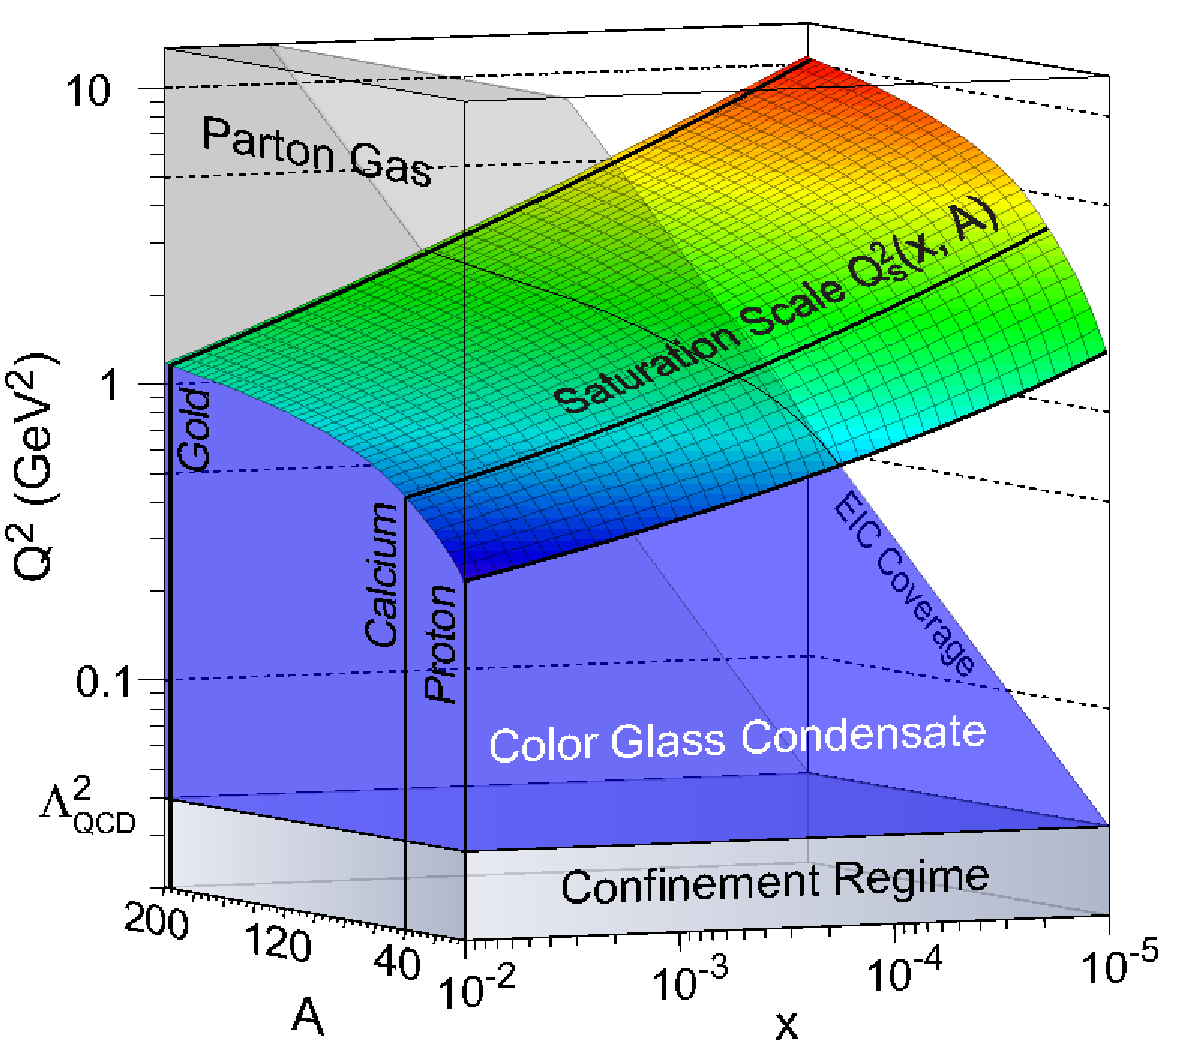
\includegraphics[width=0.85\textwidth]{images/QxA.pdf}
            }
            \only<2>{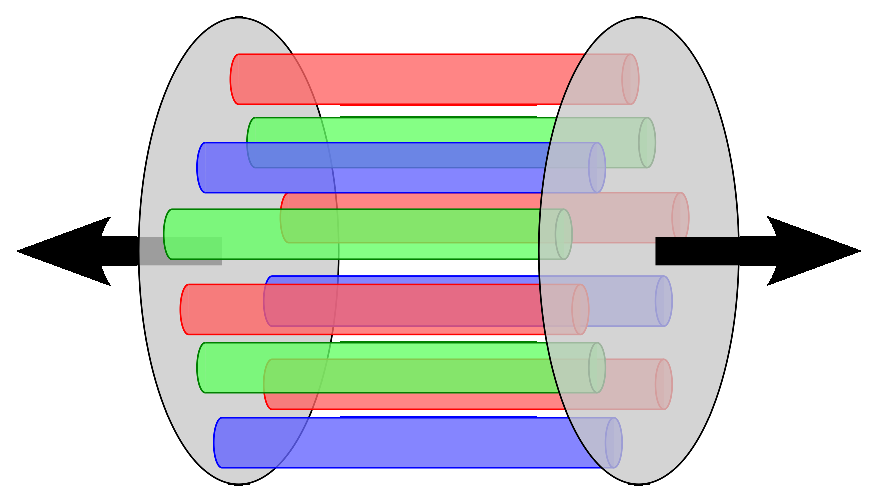
\includegraphics[width=0.85\textwidth]{images/glasma.eps}
            }
            \only<3>{\includegraphics[width=0.85\textwidth]{images/components.eps}
            }
            \only<4>{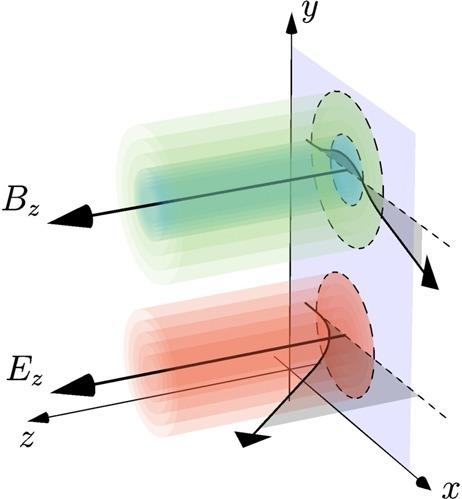
\includegraphics[width=0.7\textwidth]{images/1-s2.0-S0370269320306134-gr003_lrg.jpg}
            }
            \only<5>{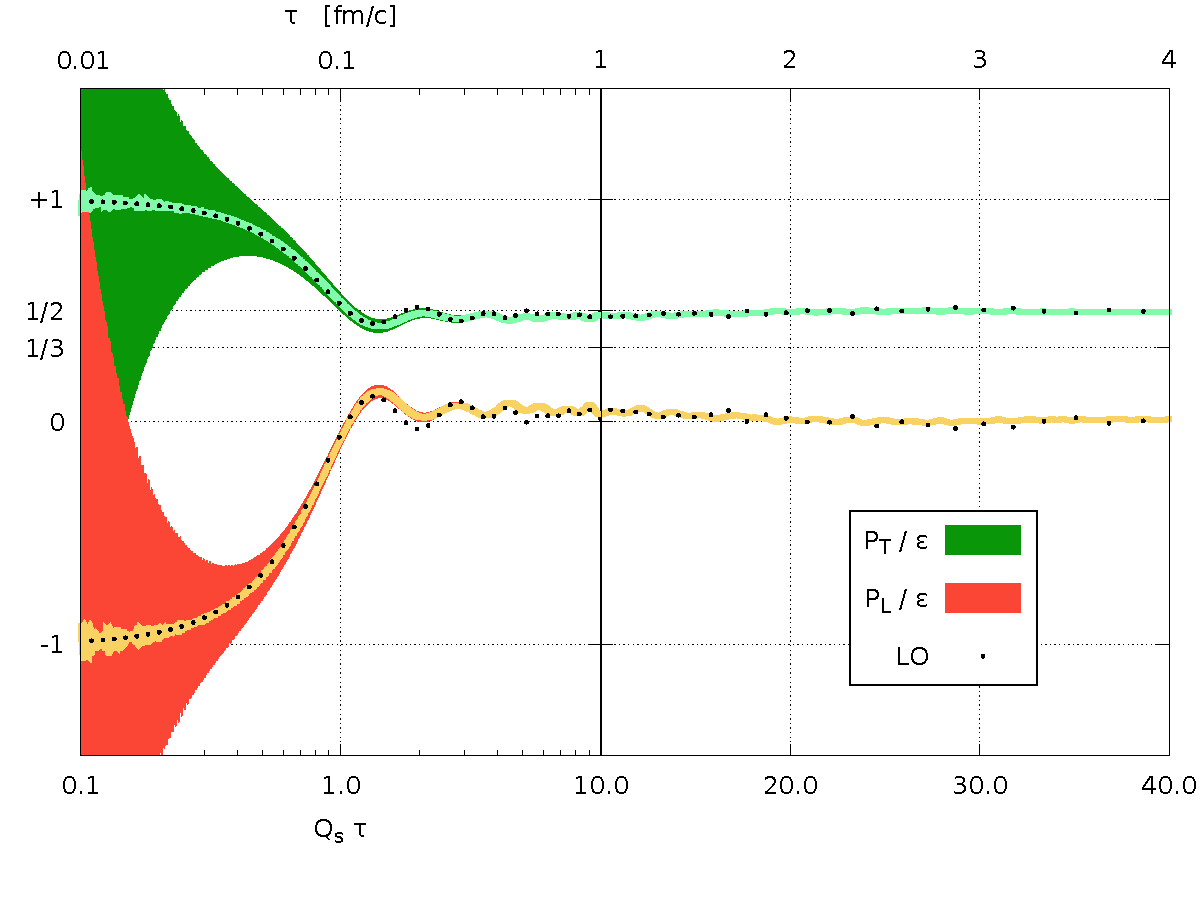
\includegraphics[width=0.85\textwidth]{images/ratio-0_1-1.pdf}
        }
        \end{figure}
        \column{.033\textwidth}
        \column{.5\textwidth}
        \vspace{0.2cm}
        \begin{center}
            \begin{itemize}
                \onslide<1,2,3,4,5>{\item Relevant scale {\color{custompink}saturation momentum $Q_s$}}
                \onslide<2,3,4,5>{\item Initial longitudinal color flux tubes}
                \onslide<3,4,5>{\item Fields {\color{customgreen}dilute} after $\tau\simeq {\color{custompink}Q}^{-1}_{\color{custompink}s}$}
                \onslide<4,5>{\item Fields arranged in {\color{customgreen}correlation domains} of $\delta x_T \simeq {\color{custompink}Q}^{-1}_{\color{custompink}s}$}
                \onslide<5>{\item Longitudinal $\neq$ transverse pressures $\Rightarrow$ {\color{pinky}anisotropy}}
            \end{itemize}
        \end{center}
        \column{.033\textwidth}
    \end{columns}
    \only<1>{\blfootnote{\scriptsize Gelis \href{https://doi.org/10.1088/1361-6633/abec2e}{{\color{customblue}\texttt{[Rept.Prog.Phys.84(2021)]}}}}}
    \only<2>{\blfootnote{\scriptsize Fukushima \href{https://doi.org/10.1088/1361-6633/80/2/022301}{{\color{customblue}\texttt{[Rept.Prog.Phys.80(2017)]}}}}}
    \only<3>{\blfootnote{\scriptsize Lappi \href{https://doi.org/10.1016/j.physletb.2006.10.017}{{\color{customblue}\texttt{[Phys.Lett.B643(2006)]}}}}}
    \only<4>{\blfootnote{\scriptsize Ipp, Müller, Schuh \href{https://doi.org/10.1016/j.physletb.2020.135810}{{\color{customblue}\texttt{[Phys.Lett.B810(2020)]}}}}}
    \only<5>{\blfootnote{\scriptsize Epelbaum, Gelis \href{https://doi.org/10.1103/PhysRevLett.111.232301}{{\color{customblue}\texttt{[Phys.Rev.Lett.111(2013)]}}}}}
\end{frame}

%%%%%%%%%%%%%%%%%%%%%%%%%%%%%%%%%%%%%%%%%%%%
%%%%%%%%%%%%%%%% SUBSECTION %%%%%%%%%%%%%%%%
%%%%%%%%%%%%%%%%%%%%%%%%%%%%%%%%%%%%%%%%%%%%

\subsection{Kinetic theory}

%%%%%%%%%%%%%%%%%%%%%%%%%%%%%%%%%%%%%%%%%
%%%%%%%%%%%%%%%%% SLIDE %%%%%%%%%%%%%%%%%
%%%%%%%%%%%%%%%%%%%%%%%%%%%%%%%%%%%%%%%%%

\setbeamertemplate{background}{
\tikz[overlay,remember picture] \node[opacity=0.1, at=(current page.center), align=center] {\\[3pt]
{\transparent{0.15}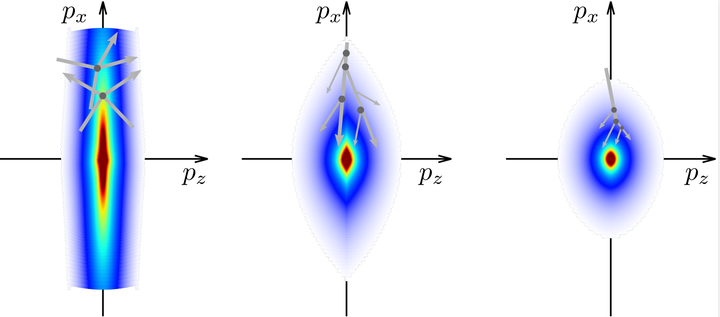
\includegraphics[height=0.6\paperheight]{images/featured_hud17e234a84b7f8be63afa171c5969276_311325_720x0_resize_lanczos_3.png}}
   };
}
\begin{frame}[plain,noframenumbering]{}
    \begin{center}
        \vspace{1cm}
        {\large\color{normal}Next stages of pre-equilibrium}\\[0.3cm]
        {\huge\color{destacado}Effective kinetic theory}
    \end{center}
\end{frame}
\setbeamertemplate{background}{}

%%%%%%%%%%%%%%%%%%%%%%%%%%%%%%%%%%%%%%%%%
%%%%%%%%%%%%%%%%% SLIDE %%%%%%%%%%%%%%%%%
%%%%%%%%%%%%%%%%%%%%%%%%%%%%%%%%%%%%%%%%%

\setbeamertemplate{background}{
\tikz[overlay,remember picture] \node[at=(current page.center), align=center] {\\[3pt]
{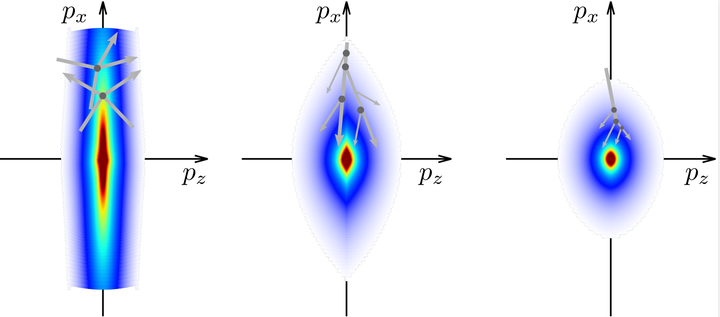
\includegraphics[height=0.6\paperheight]{images/featured_hud17e234a84b7f8be63afa171c5969276_311325_720x0_resize_lanczos_3.png}}};
}
\begin{frame}[plain,noframenumbering]{}
    \blfootnote{\scriptsize Kurkela, Mazeliauskas, Paquet, Schlichting, Teaney \href{https://journals.aps.org/prc/abstract/10.1103/PhysRevC.99.034910}{{\color{customblue}\texttt{[Phys.Rev.C99(2019)]}}}}
\end{frame}
\setbeamertemplate{background}{}

%%%%%%%%%%%%%%%%%%%%%%%%%%%%%%%%%%%%%%%%%
%%%%%%%%%%%%%%%%% SLIDE %%%%%%%%%%%%%%%%%
%%%%%%%%%%%%%%%%%%%%%%%%%%%%%%%%%%%%%%%%%

\setbeamertemplate{background}{
\tikz[overlay,remember picture] \node[at=(current page.center), align=center] {\\[40pt]
{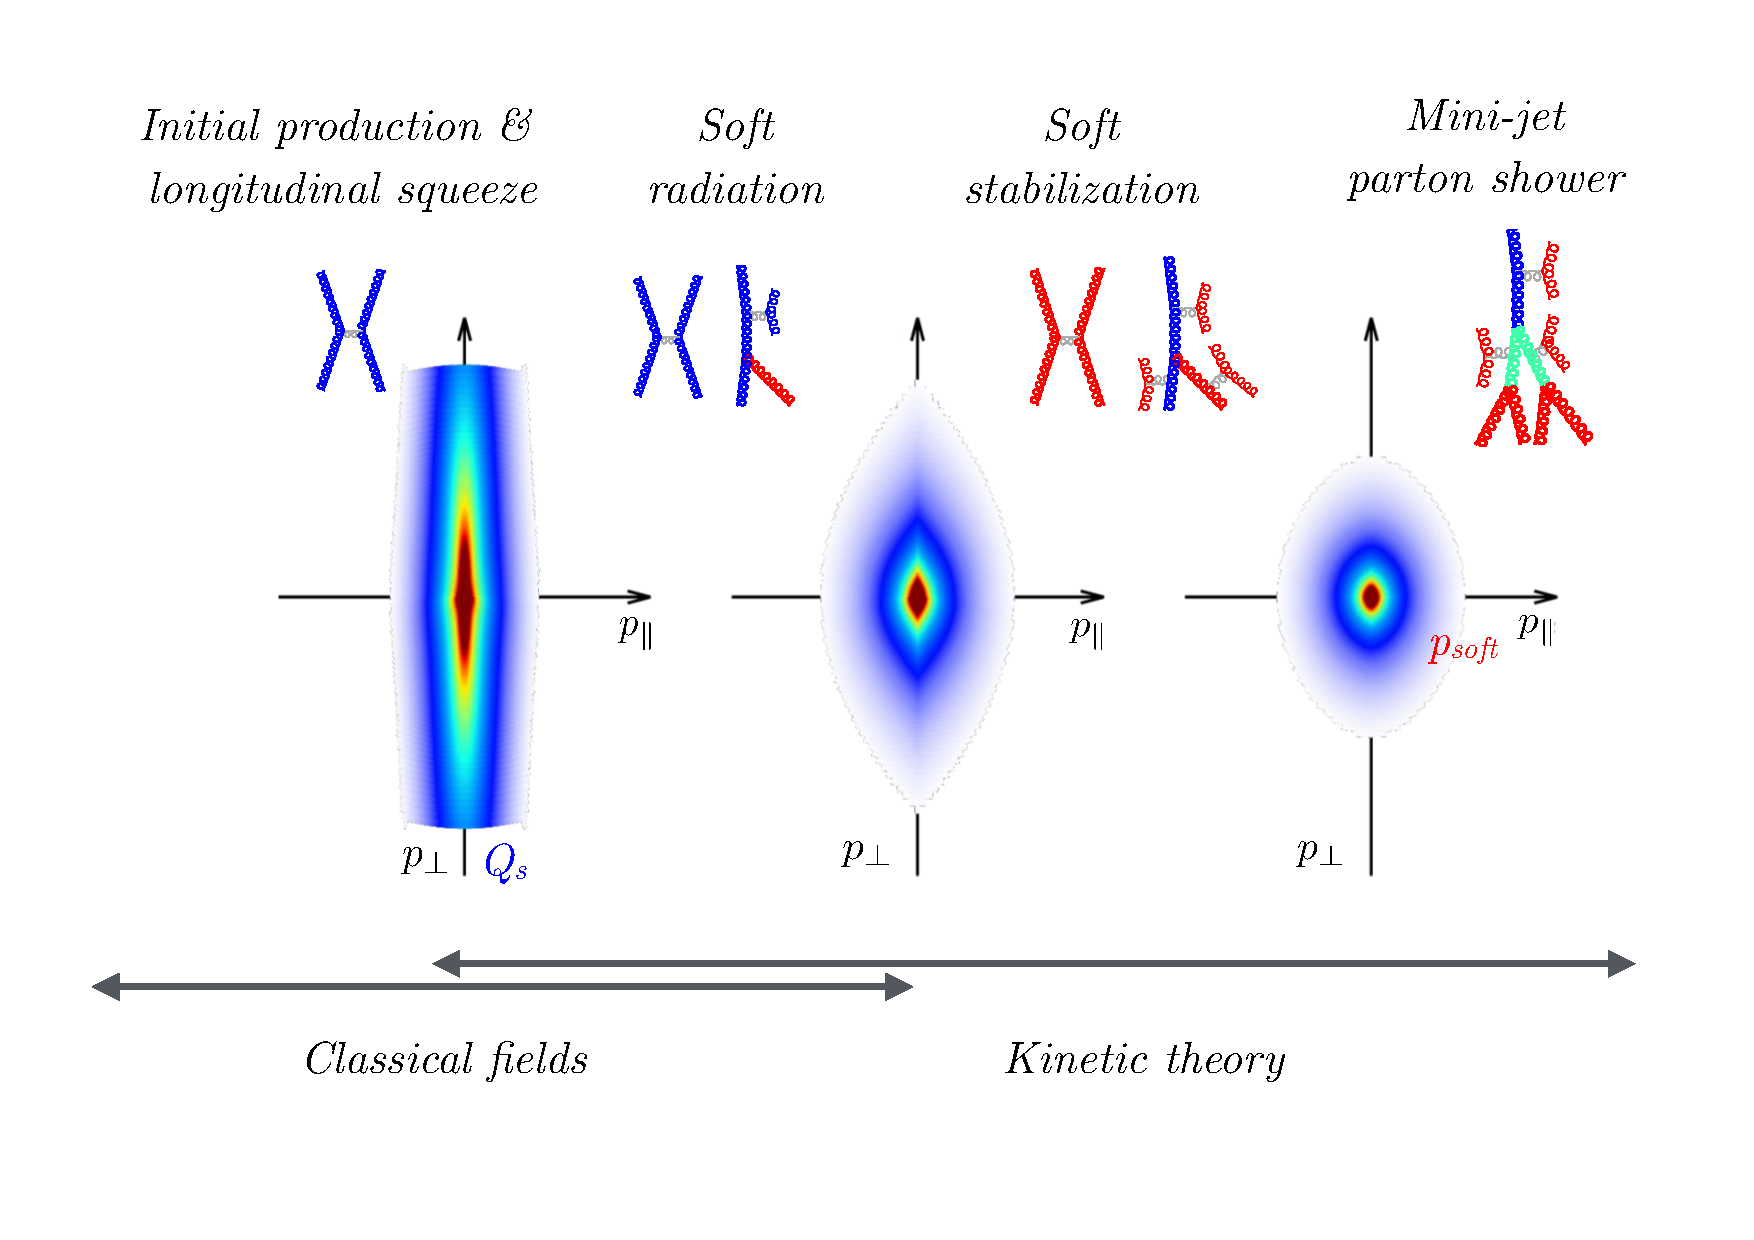
\includegraphics[height=0.65\paperheight]{images/CARTOON_BUP_SS.pdf}}};
}
\begin{frame}
    \frametitle{Bottom-up thermalization}
    \framesubtitle{Equilibration at weak coupling}
    \blfootnote{\scriptsize Schlichting, Teaney \href{hhttps://doi.org/10.1146/annurev-nucl-101918-023825}{{\color{customblue}\texttt{[Ann.Rev.Nucl.Part.Sci.69(2019)]}}}}
\end{frame}
\setbeamertemplate{background}{}

% \begin{frame}
%     \frametitle{Effective kinetic theory}
%     \framesubtitle{\`{A} la AMY\footnote{\scriptsize Arnold, Moore, Yaffe \href{https://iopscience.iop.org/article/10.1088/1126-6708/2003/01/030}{{\color{customblue}\texttt{[JHEP01(2003)]}}}} and KZ\footnote{\scriptsize Kurkela, Zhu \href{https://journals.aps.org/prl/abstract/10.1103/PhysRevLett.115.182301}{{\color{customblue}\texttt{[Phys.Rev.Lett.115(2015)]}}}}}
%     \begin{columns}[onlytextwidth,t]
%         \column{.02\textwidth}
%        \column{.46\textwidth}
%        \begin{figure}
%             \centering
%             \captionsetup{justification=centering}
%             \caption{\scriptsize Trajectories for different initial conditions\footnotemark[2]}
%             \includegraphics[width=0.85\textwidth]{images/cdplot_4.eps}
%         \end{figure}
%         \column{.02\textwidth}
%         \column{.5\textwidth}
%         \vspace{0.2cm}
%         \begin{itemize}
%             % \item Gluon distribution function $f(t,\boldsymbol{p})$
%             \item Boltzmann equation\\
%                 \renewcommand{\eqnhighlightheight}{\vphantom{\mathcal{D}_\mu}\mathstrut}\begin{equation*}
%                 -\frac{\mathrm{d}}{\mathrm{d} \tau}\eqnmark[pinky]{fp}{f_{\boldsymbol{p}}}=\Big(
%                 \eqnmark[ming]{c12}{\mathcal{C}_{1 \leftrightarrow 2}}+ \eqnmark[ming]{c22}{\mathcal{C}_{2 \leftrightarrow 2}}+ \eqnmark[starrysecond]{cexp}{\mathcal{C}_{\mathrm{exp}}}\Big)({\color{pinky}f_{\boldsymbol{p}}})
%                 \end{equation*}
%                 \annotate[yshift=-2.2em]{below, right}{fp}{\scriptsize distribution function}
%                 \annotatetwo[yshift=+1em]{above}{c12}{c22}{\scriptsize collision terms}
%                 \annotate[yshift=-0.7em]{below, left}{cexp}{\scriptsize longitudinal expansion}
%                 \\[20pt]
%             {\footnotesize \item Soft scale $m_D$ $\ll$ hard scale $Q_s$
%             \item Overoccupied $f\sim 1/\alpha_s$ at $Q_s\tau\sim 1$
%             \item Boost-invariance $p_z\ll p_T$}
%         \end{itemize}
%         \column{.02\textwidth}
%     \end{columns}
% \end{frame}

% \begin{frame}
%     \frametitle{Stages of bottom-up}
%     \framesubtitle{Classical fields, soft particles, energy loss}
%     \begin{columns}[onlytextwidth,t]
%         \column{.02\textwidth}
%        \column{.44\textwidth}
%        \begin{figure}
%             \centering
%             \captionsetup{justification=centering}
%             \only<1>{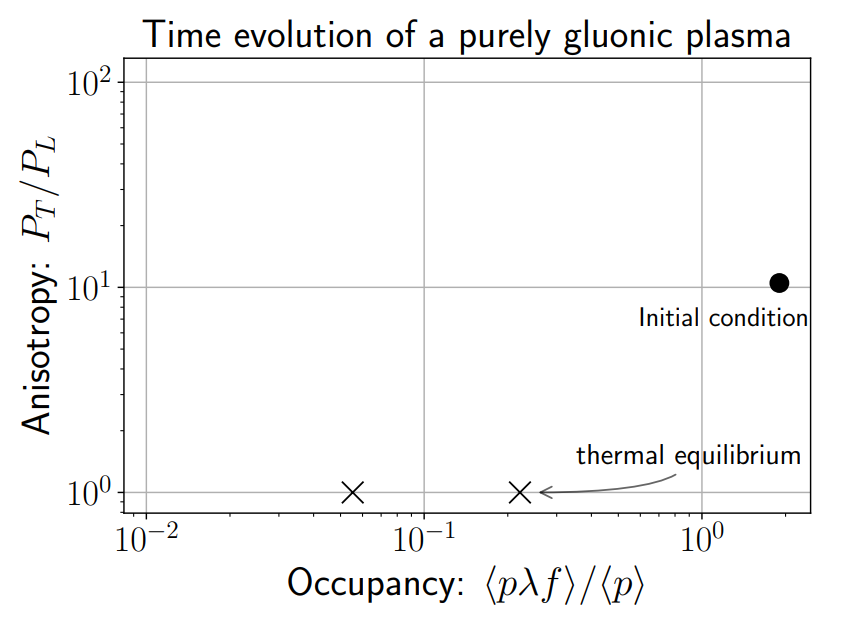
\includegraphics[width=0.95\textwidth]{images/Screenshot from 2024-08-23 15-55-35.png}}
%             \only<2>{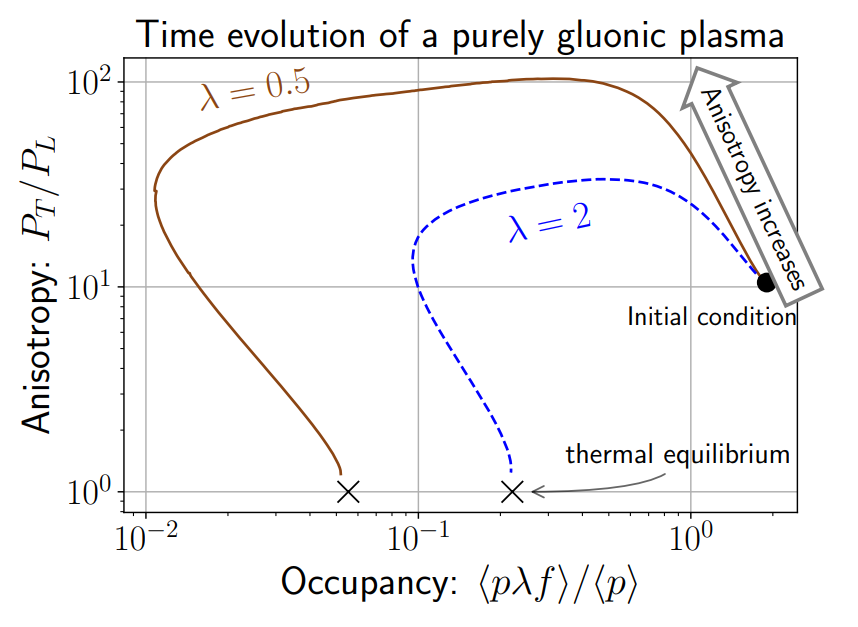
\includegraphics[width=0.95\textwidth]{images/Screenshot from 2024-08-23 15-55-47.png}}
%             \only<3>{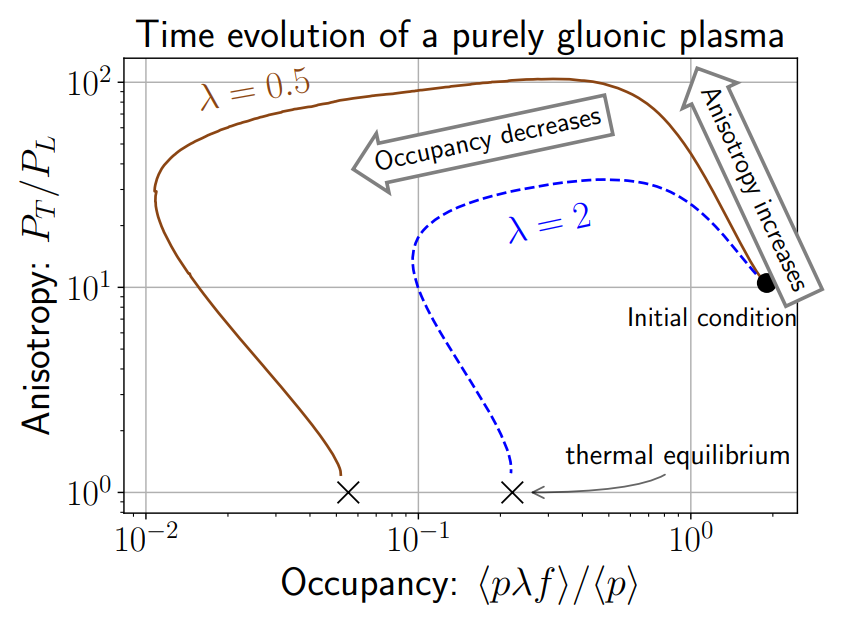
\includegraphics[width=0.95\textwidth]{images/Screenshot from 2024-08-23 15-55-53.png}}
%             \only<4>{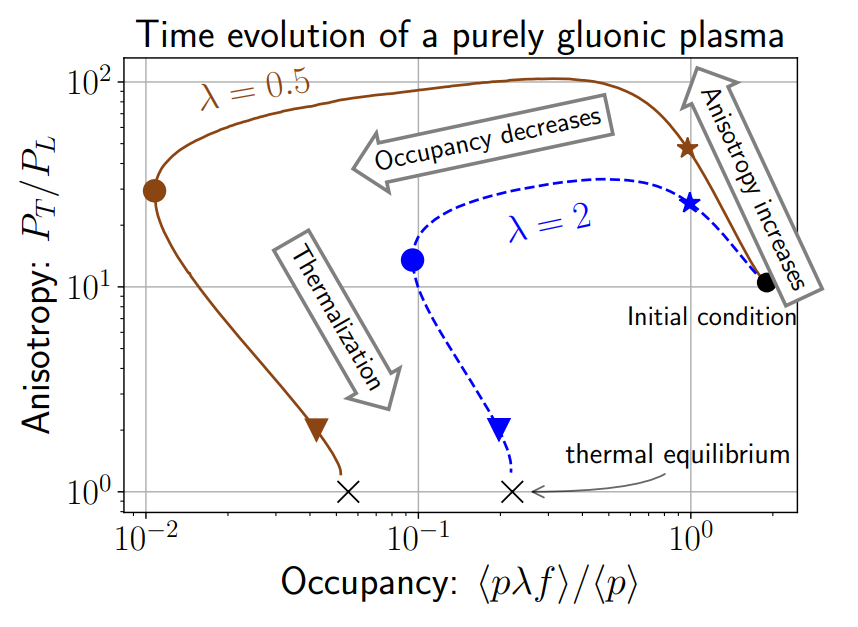
\includegraphics[width=0.95\textwidth]{images/Screenshot from 2024-08-23 15-56-03.png}}
%             \only<5>{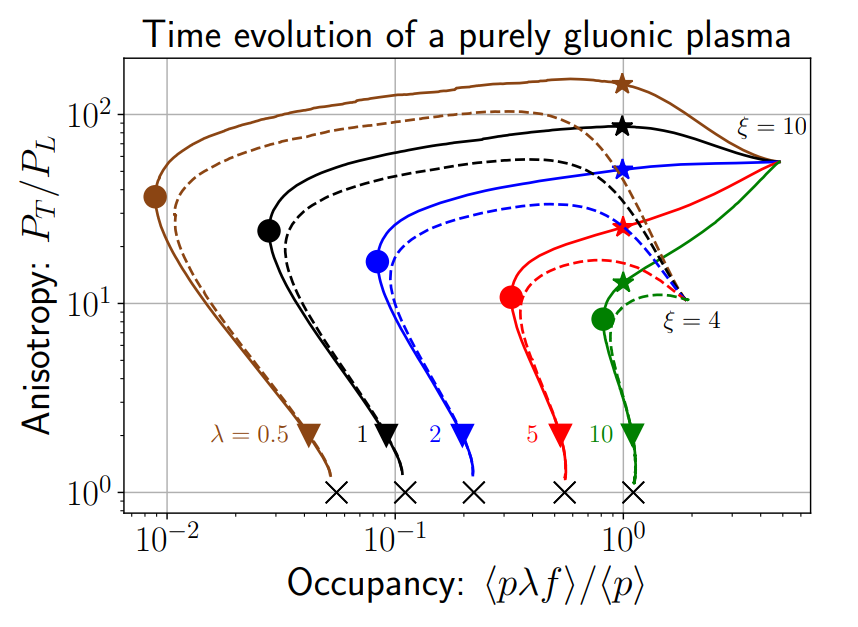
\includegraphics[width=0.95\textwidth]{images/Screenshot from 2024-08-23 15-56-07.png}}
%         \end{figure}
%         \column{.02\textwidth}
%         \column{.5\textwidth}
%         \vspace{0.2cm}
%         \begin{center}
%             \begin{itemize}
%                 \onslide<1,2,3,4,5>{\item Stage $\boldsymbol{\circ}$\\ 
%                 Overoccupied gluon fields\\
%                 Anisotropy $\xi$, coupling $\lambda=4\pi N_c\alpha_s$}
%                 \onslide<2,3,4,5>{\item {\color{ming}Stage $\boldsymbol{\star}$} \\
%                 Maximum anisotropy, hard modes}
%                 \onslide<3,4,5>{\item {\color{ming}Stage $\bullet$} \\
%                 Minimum occupancy, bath of soft modes}
%                 \onslide<4,5>{\item {\color{ming}Stage $\mathsmaller{\blacktriangledown}$} \\
%                 Almost isotropic, hard modes radiated}
%                 \onslide<5>{\\ Thermalization $\tau_{\mathrm{BMSS}}\sim \alpha_s^{-13/5}Q_s^{-1}$}
%             \end{itemize}
%         \end{center}
%         \column{.02\textwidth}
%     \end{columns}
% \end{frame}

% \begin{frame}[noframenumbering]
%     \frametitle{Stages of bottom-up}
%     % \framesubtitle{Many studies}
%     \begin{center}
%        \begin{figure}
%             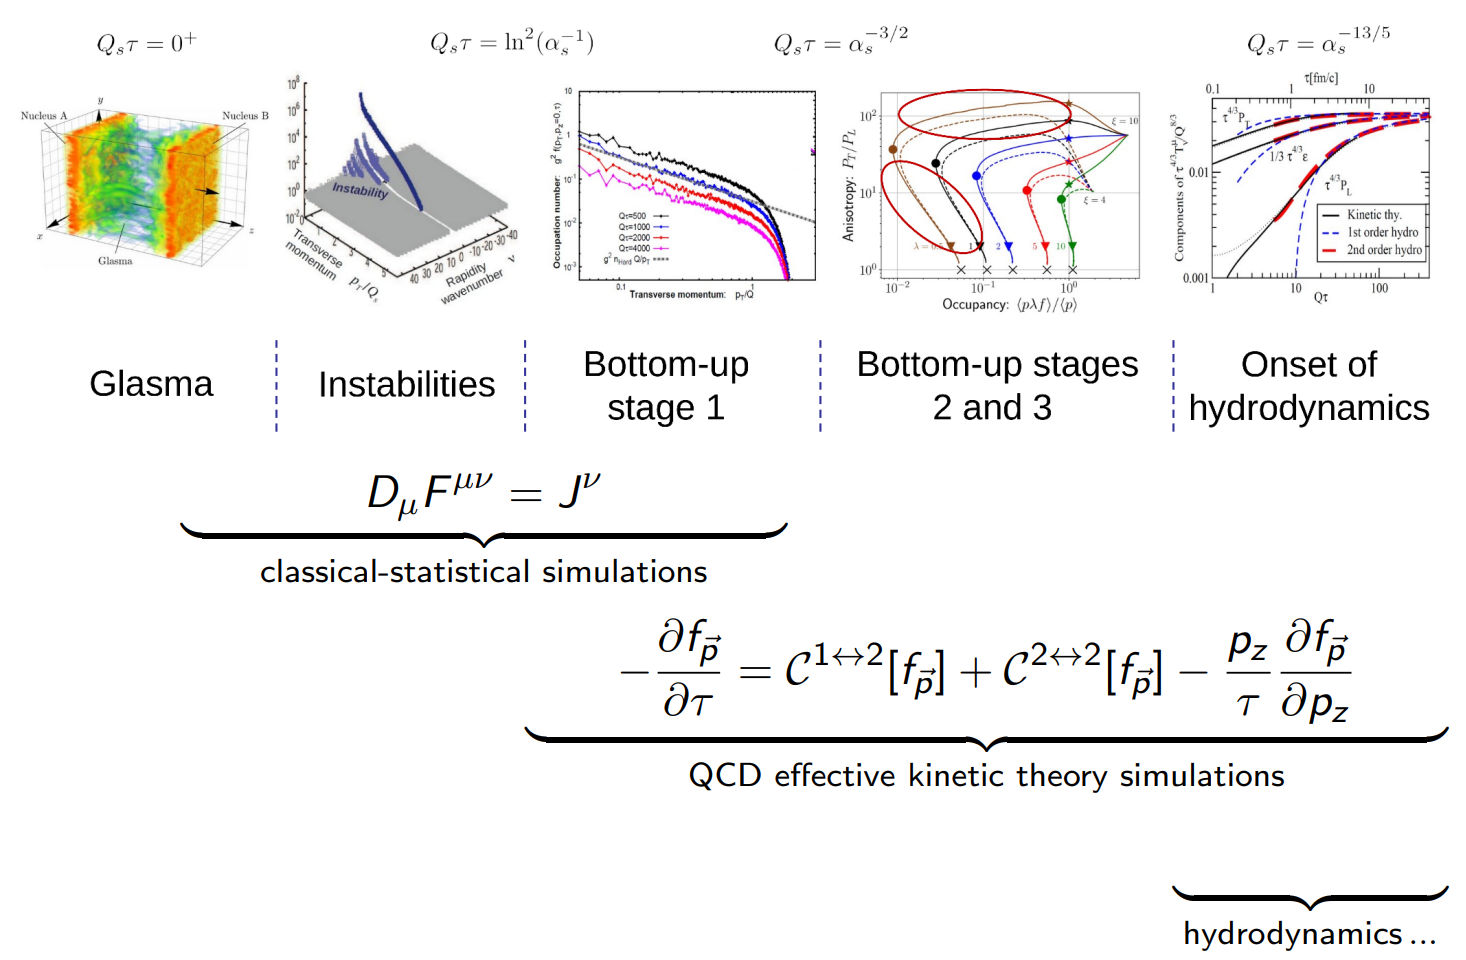
\includegraphics[width=1.4\textheight]{images/Screenshot from 2024-08-23 16-32-50.png}
%         \end{figure}
%         {\color{red}Add references}
%     \end{center}
% \end{frame}

% % \setbeamertemplate{background}{
% % \tikz[overlay,remember picture] \node[at=(current page.center), align=center] {\\[40pt]
% % {\transparent{0.2}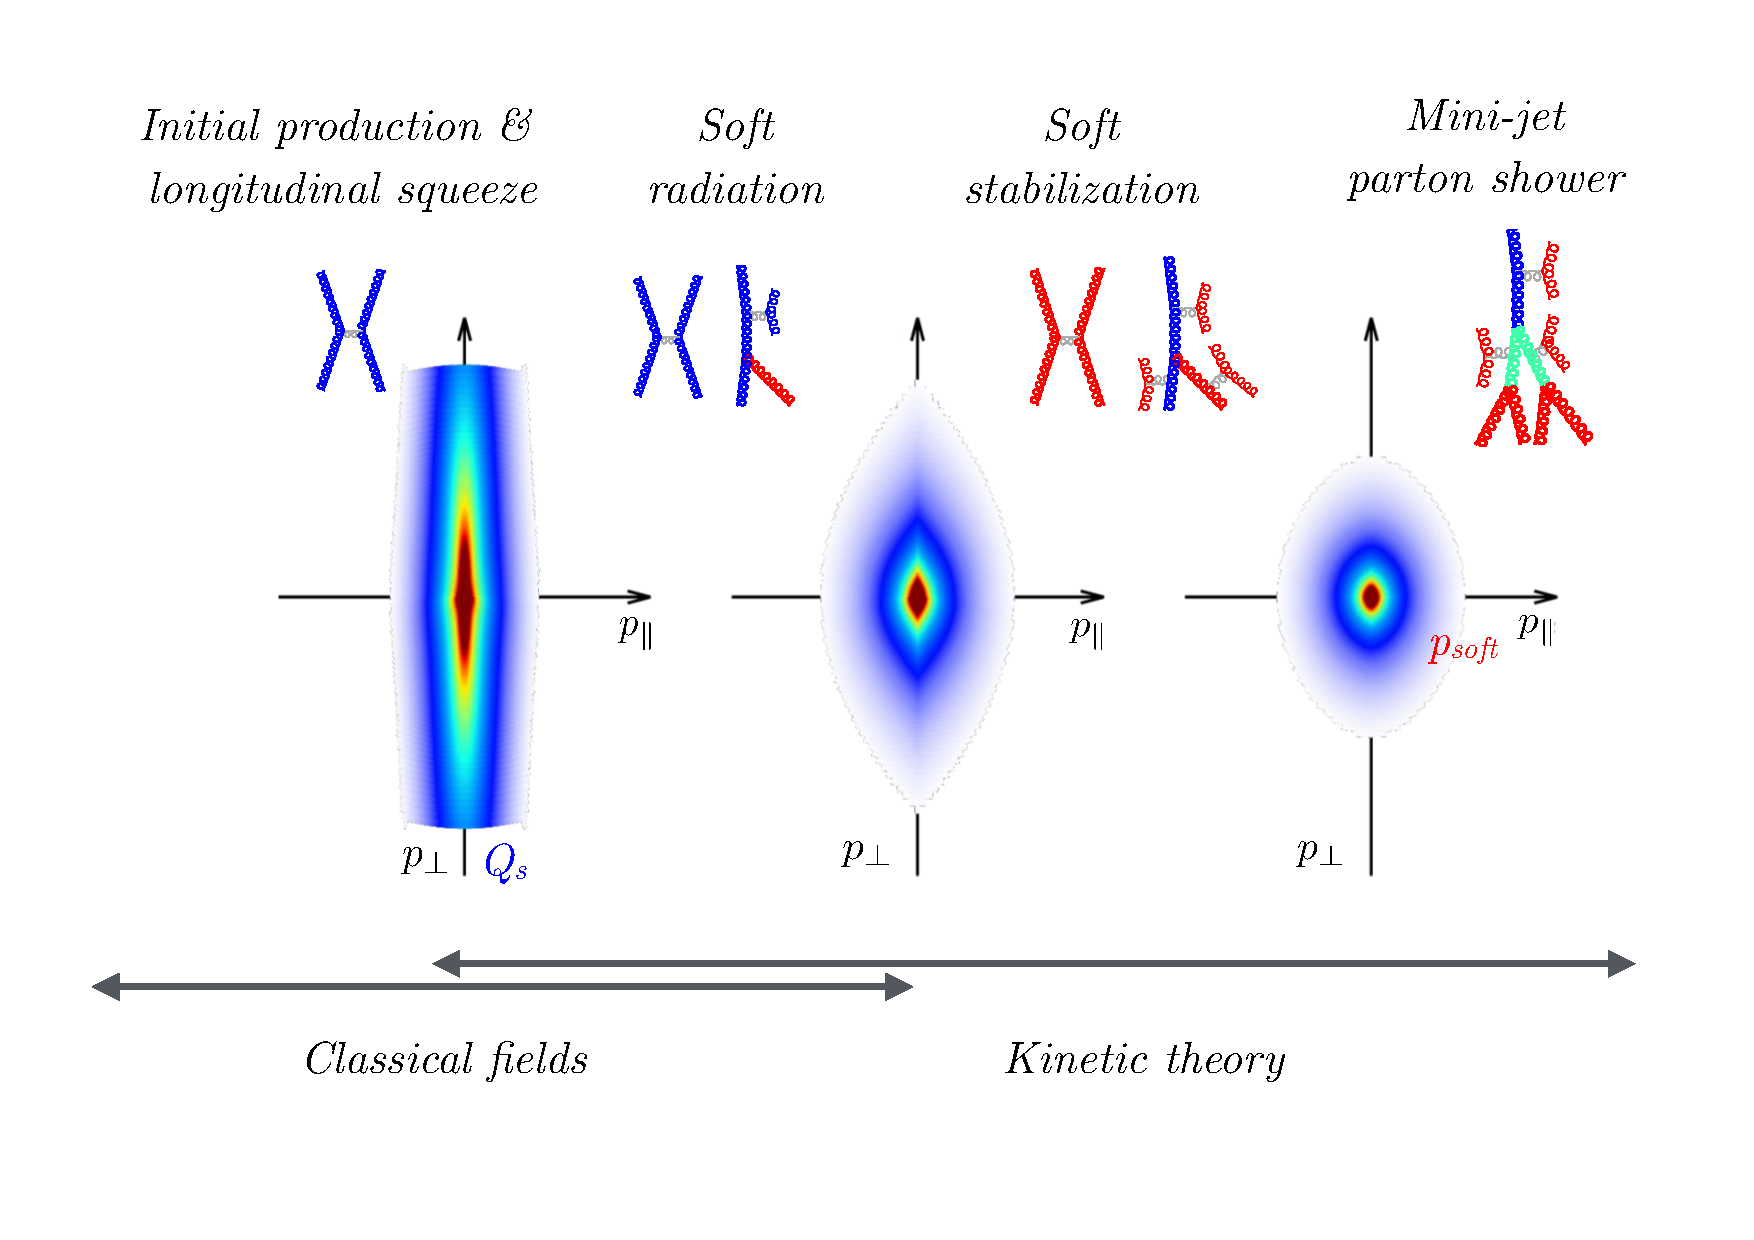
\includegraphics[height=0.65\paperheight]{images/CARTOON_BUP_SS.pdf}}
% %    \\[10pt]  
% %    {\transparent{5}\footnotesize\itshape Figure from  S. Schlichting, D. Teaney \href{https://arxiv.org/abs/1908.02113}{{\color{lightgray}\texttt{[1908.02113]}}}}};
% % }
% % \begin{frame}
% %     \frametitle{Bottom-up thermalization}
% %     \framesubtitle{Equilibration at weak coupling}
% %     \begin{center}
% %         {\huge Weak coupling parametric estimate}\\[20pt]
% %         {\footnotesize\itshape Other frameworks for pre-equilibrium dynamics are not included in this talk\\
% %         {\color{red}Add references}}
% %     \end{center}
% % \end{frame}
% % \setbeamertemplate{background}{}


% %%%%%%%%%%%%%%%%%%%%%%%%%%%%%%%%%%%%%%%%%%%
% %%%%%%%%%%%%%%%% SECTION 3 %%%%%%%%%%%%%%%%
% %%%%%%%%%%%%%%%%%%%%%%%%%%%%%%%%%%%%%%%%%%%

% \section{{\color{jyublue}Heavy quarks} in pre-equilibrium}

% \setbeamertemplate{background}{
% \tikz[overlay,remember picture] \node[opacity=0.1, at=(current page.center), align=center] {
%     % \\[-20pt]
%     \\[45pt]
% {\transparent{0.3}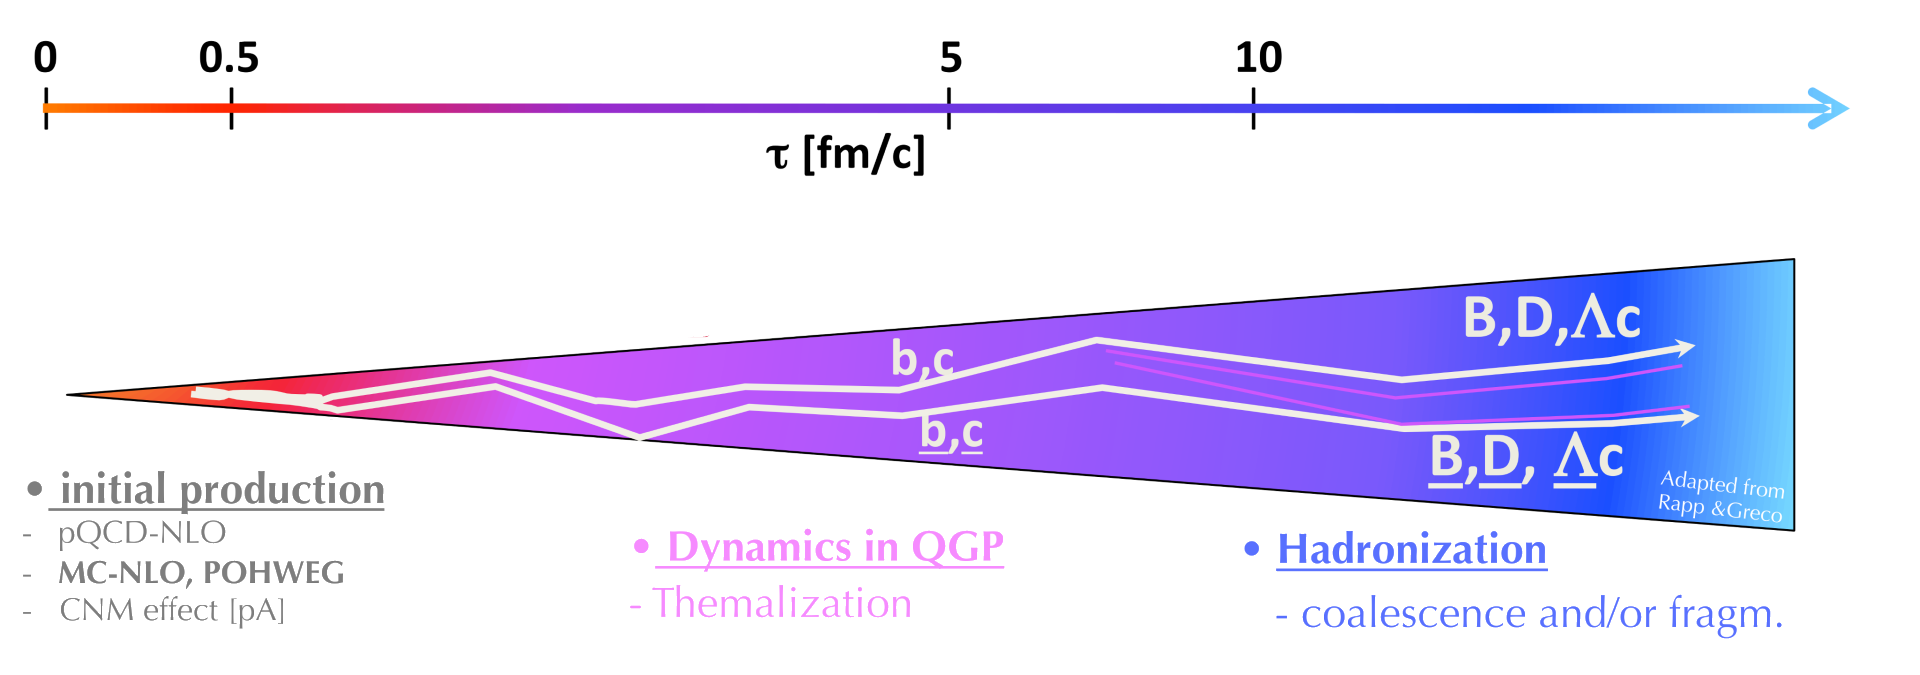
\includegraphics[height=0.55\paperheight]{images/Greco-HF-Theory-HP2020-v-5_edit.png}}
%    \\[10pt]  
%    {\transparent{0.3}\footnotesize\itshape Figure credits to V. Greco}};
% }
% \begin{frame}[plain,noframenumbering]{}
%     \begin{center}
%         \vspace{1cm}
%         {\huge\color{destacado}Heavy quarks in pre-equilibrium}
%     \end{center}
% \end{frame}
% \setbeamertemplate{background}{}


% \subsection{Glasma}

% \setbeamertemplate{background}{
% \tikz[overlay,remember picture] \node[opacity=0.1, at=(current page.center), align=center] {\\[10pt]
% {\transparent{0.1}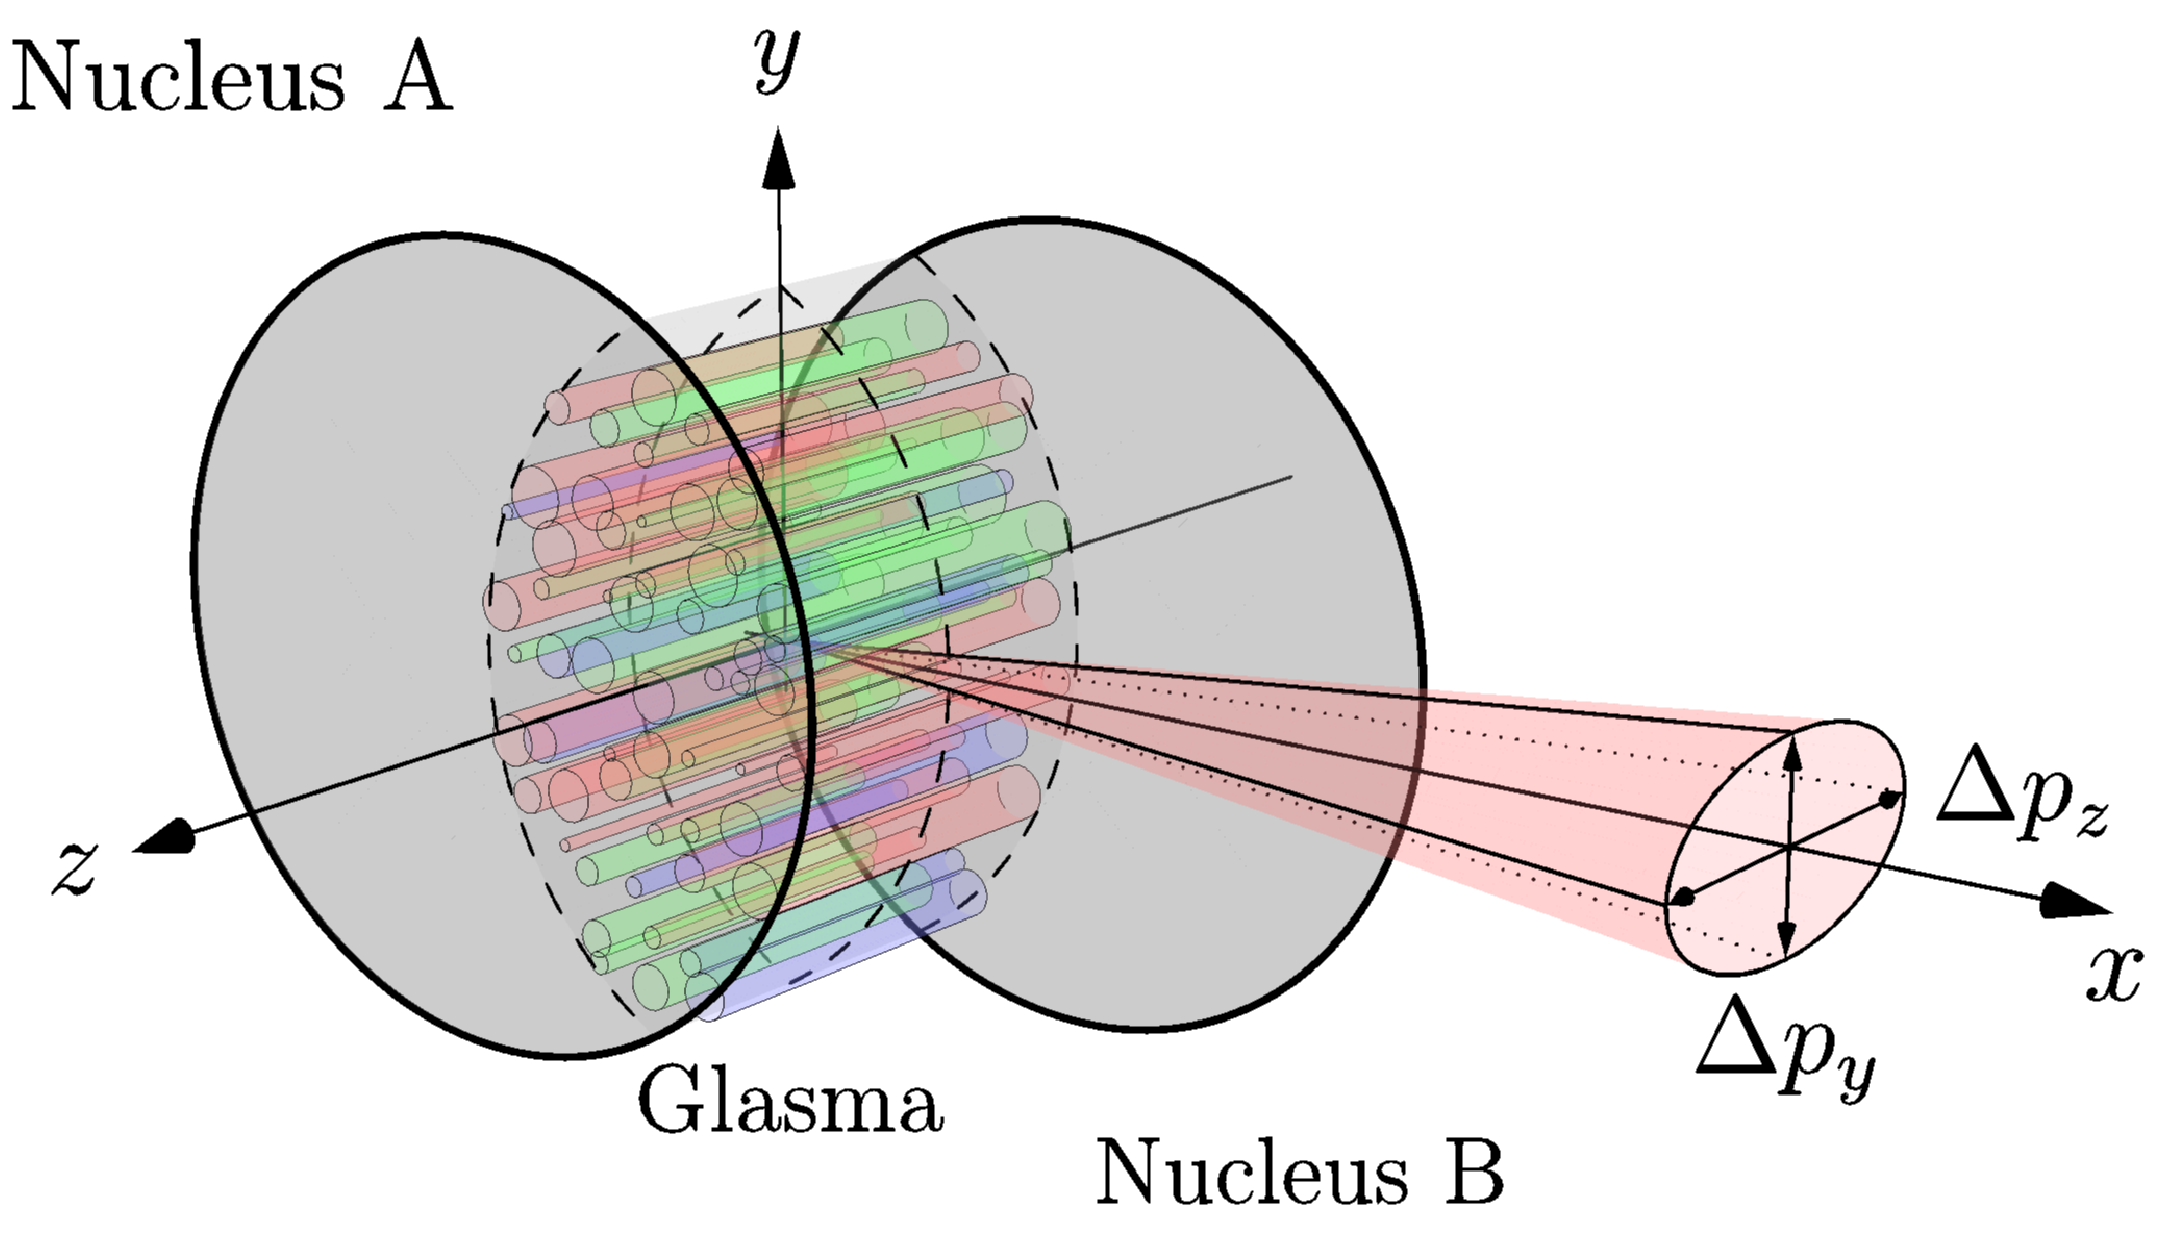
\includegraphics[height=0.7\paperheight]{images/momentum_broadening_flipped.pdf}}
%    \\[10pt]  
%    {\transparent{0.3}\footnotesize\itshape Figure from  A. Ipp, D. Müller, D. Schuh \href{https://arxiv.org/abs/2009.14206}{{\color{lightgray}\texttt{[2009.14206]}}}}};
% }

% \setbeamertemplate{itemize item}{\raisebox{0.2em}{\scalebox{0.7}{${\color{normal}\blacktriangleright}$}}} 

% \begin{frame}[plain,noframenumbering]{}
%     \begin{center}
%         \vspace{1cm}
%         {\large\color{normal}Initial stage of pre-equilibrium}\\[0.3cm]
%         {\huge\color{destacado}Heavy quarks in glasma}\\[0.3cm]
%         {\large\color{normal}
%         \begin{center}
%             % \begin{minipage}{0.45\textwidth}
%             % \begin{itemize}
%             %     \item Momentum broadening $\langle \delta p^2\rangle$
%             %     \item Transport coefficient $\kappa$
%             %     \item Observables $R_{AA}$, $v_2$, $\mathcal{C}(\Delta\phi)$
%             % \end{itemize}
%             % \end{minipage}
%             \begin{columns}
%                 \begin{column}{0.066\textwidth}\end{column}
%                 \begin{column}{0.35\textwidth}
%                     \centering
%                     \setbeamertemplate{itemize item}{\raisebox{0.2em}{\scalebox{0.7}{${\color{ming}\blacktriangleright}$}}} 
%                     {\Large\color{ming} Approaches}
%                     \begin{itemize}
%                         \item Numerical trajectories
%                         \item Correlator method
%                     \end{itemize}
%                 \end{column}
%                 \begin{column}{0.066\textwidth}\end{column}
%                 \begin{column}{0.45\textwidth}
%                     \centering
%                     \\[10pt]
%                     \setbeamertemplate{itemize item}{\raisebox{0.2em}{\scalebox{0.7}{${\color{pinky}\blacktriangleright}$}}} 
%                     {\Large\color{pinky} Quantities}
%                     \begin{itemize}
%                         \item Momentum broadening $\langle \delta p^2\rangle$
%                         \item Transport coefficient $\kappa$
%                         \item Observables $R_{AA}$, $v_2$, $\mathcal{C}(\Delta\phi)$
%                     \end{itemize}
%                 \end{column}
%                 \begin{column}{0.066\textwidth}\end{column}
%             \end{columns}
%         \end{center}
%         }
%         % \\[0.3cm]
%     \end{center}
% \end{frame}
% \setbeamertemplate{background}{}

% \begin{frame}
%     \frametitle{Particles in Yang-Mills fields}
%     \framesubtitle{Wong's equations of motion}
%         \setbeamertemplate{itemize item}{\raisebox{0.2em}{\scalebox{0.7}{${\color{ming}\blacktriangleright}$}}} 
%         \begin{itemize}
%             \item \begin{center}{{\color{ming}Approach}: {\color{ming}numerical trajectories} of classical particles in glasma fields} \end{center}
%         \end{itemize} 
%    \begin{center}
%        Wong's equations $\leftrightarrow$ classical equations of motion for particles $({\color{customblue}x^\mu},{\color{customred}p^\mu},{\color{customyellow}Q})$ \\
%     evolving in a Yang-Mills background field ${\color{starrysecond}A^\mu}$
%    \end{center} 
%         \vspace{1cm}
%         \renewcommand{\eqnhighlightheight}{\vphantom{x}}
%         \begin{equation*}
%             \frac{\d}{\d\hspace{-0.1cm}\eqnmark[destacado]{tau}{\boldsymbol{\tau}}\hspace{-0.2cm}}\eqnmark[customblue]{xmu}{x^\mu}=\frac{{\color{customred}p^\mu}}{\eqnmark[destacado]{m}{m}},\qquad \eqnmark[destacado]{Ddtau}{\frac{\mathrm{D}}{\d\boldsymbol{\tau}}}\hspace{-0.2cm}\eqnmark[customred]{pmu}{p^\mu}=2\hspace{-0.1cm}\eqnmark[destacado]{g}{g}\hspace{-0.1cm}\tr{{\color{customyellow}Q}F^{\mu\nu}[\hspace{-0.1cm}\eqnmark[starrysecond]{amu}{A^\mu}\hspace{-0.1cm}]}\frac{{\color{customred}p_\nu}}{m},\qquad 
%             \underbrace{\frac{\d}{\d\boldsymbol{\tau}}\hspace{-0.1cm}\eqnmark[customyellow]{Q}{Q}\hspace{-0.1cm}=-\mathrm{i}g [{\color{starrysecond}A_\mu},{\color{customyellow}Q}]\,\frac{{\color{customred}p^\mu}}{m}}_{\substack{\text{\footnotesize color rotation}\,\rightarrow\,{\color{customgreen}\mathcal{U}}\in\,\mathrm{SU(3)} \\[0.2cm] {\color{customyellow}Q}(\boldsymbol{\tau})=\,{\color{customgreen}\mathcal{U}}(\boldsymbol{\tau},\boldsymbol{\tau}^\prime){\color{customyellow}Q}(\boldsymbol{\tau^\prime})\,{\color{customgreen}\mathcal{U}^\dagger}(\boldsymbol{\tau},\boldsymbol{\tau}^\prime)}}
%             \end{equation*}
%             \annotate[yshift=1.2em]{above}{xmu}{coordinate}
%             \annotate[yshift=1.2em]{above}{pmu}{momentum}
%             \annotate[yshift=-0.5em]{below, right}{m}{\tiny mass}
%             \annotate[yshift=-1.5em]{below, right}{Ddtau}{\tiny covariant derivative}
%             \annotate[yshift=-1.5em]{below, right}{tau}{\tiny proper time}
%             \annotate[yshift=-0.7em]{below, right}{g}{\tiny coupling constant}
%             \annotate[yshift=1.2em]{above}{Q}{color charge}
%             \annotate[yshift=1.2em]{above, right}{amu}{gauge field}
%     %    \\
%         % \begin{center}
%         %     Symplectic numerical solver $\xrightarrow{\mathrm{assures}}$ ${\color{customyellow}Q}\in\mathrm{SU(3)}$, conservation of Casimir invariants 
%         % \end{center} 
% \end{frame}

% \begin{frame}[noframenumbering]
%     \frametitle{Particles in Yang-Mills fields}
%     \framesubtitle{Vizualizing the trajectories\footnote{\scriptsize Avramescu, Băran, Greco, Ipp, Müller, Ruggieri  \href{https://journals.aps.org/prd/abstract/10.1103/PhysRevD.107.114021}{{\color{customblue}\texttt{[Phys.Rev.D107(2023)]}}}}}
%     \vspace{-0.5cm}
%     \begin{columns}[onlytextwidth,t]
%         \column{.025\textwidth}
%        \column{.3\textwidth}
%                 \begin{center}
%                     Change of coordinates 
%                 \end{center}
%                 \vspace{-20pt}
%                 \begin{figure}[!hbt]
%                     \centering
%                 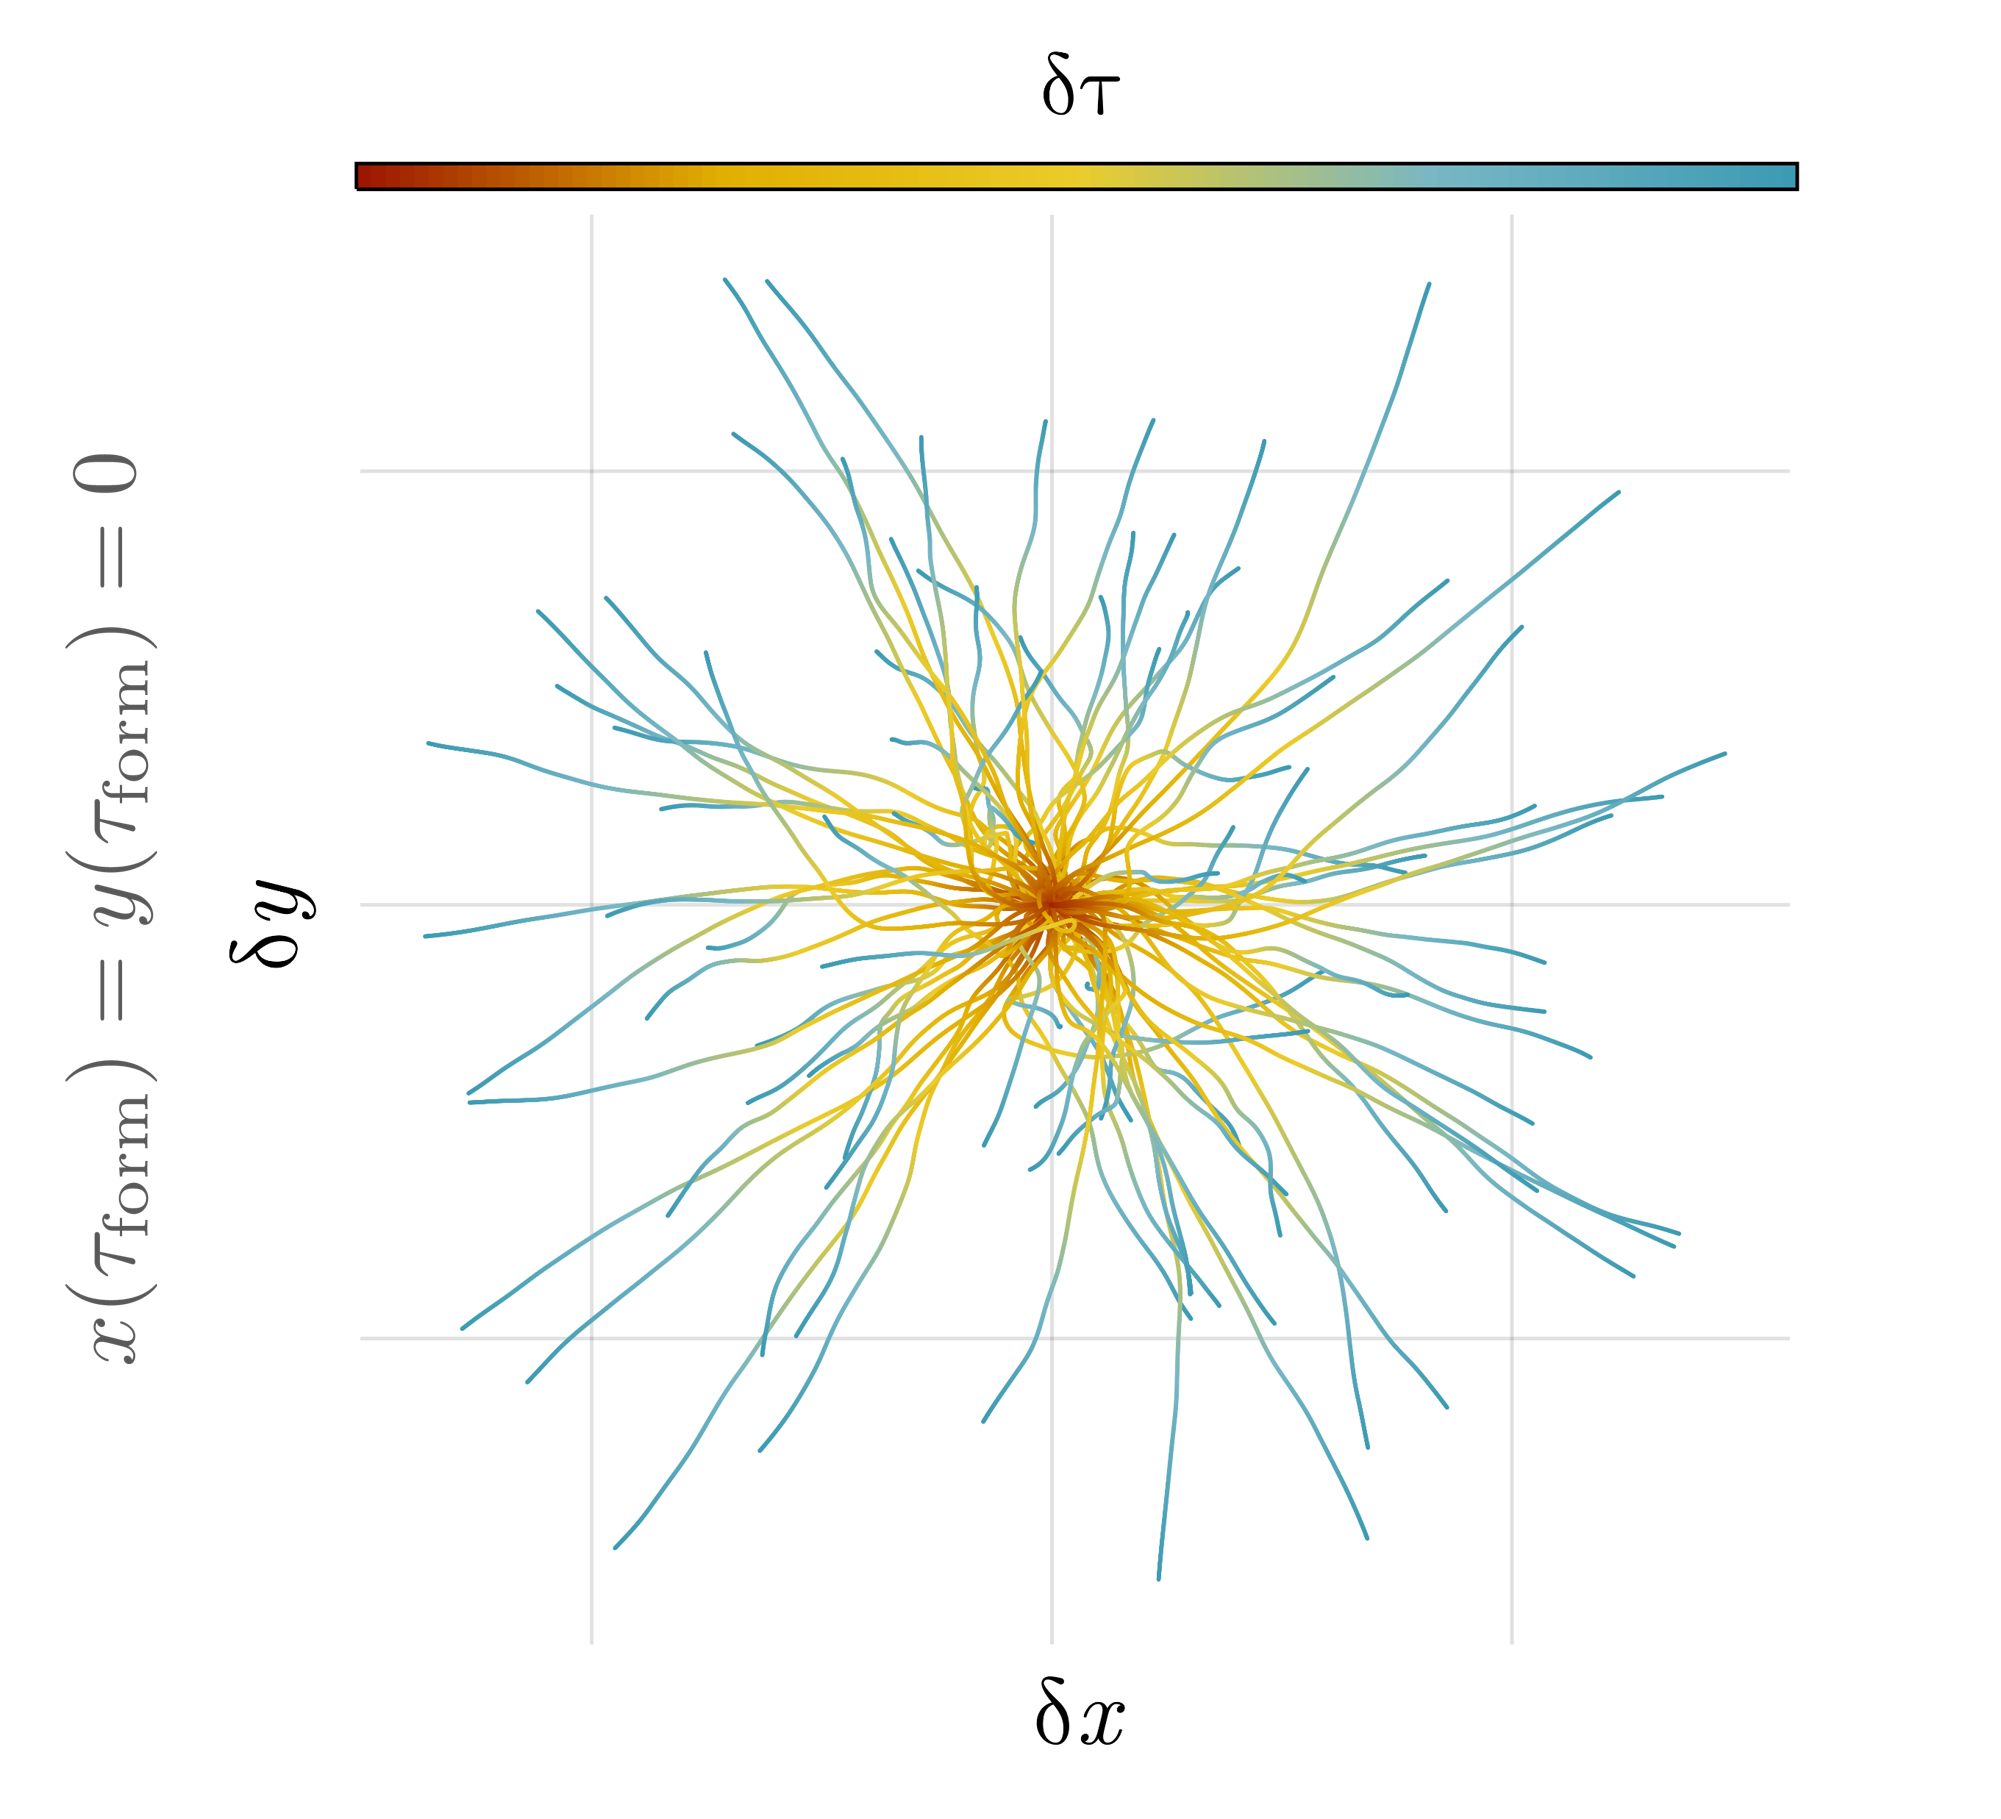
\includegraphics[width=1.1\columnwidth]{images/wong_coord.png}
%                 \end{figure}
%                 \column{.025\textwidth}
%         \column{.3\textwidth}
%             \begin{center}
%                 Color Lorentz force
%             \end{center}
%             \vspace{-20pt}
%             \begin{figure}[!hbt]
%                 \centering
%                 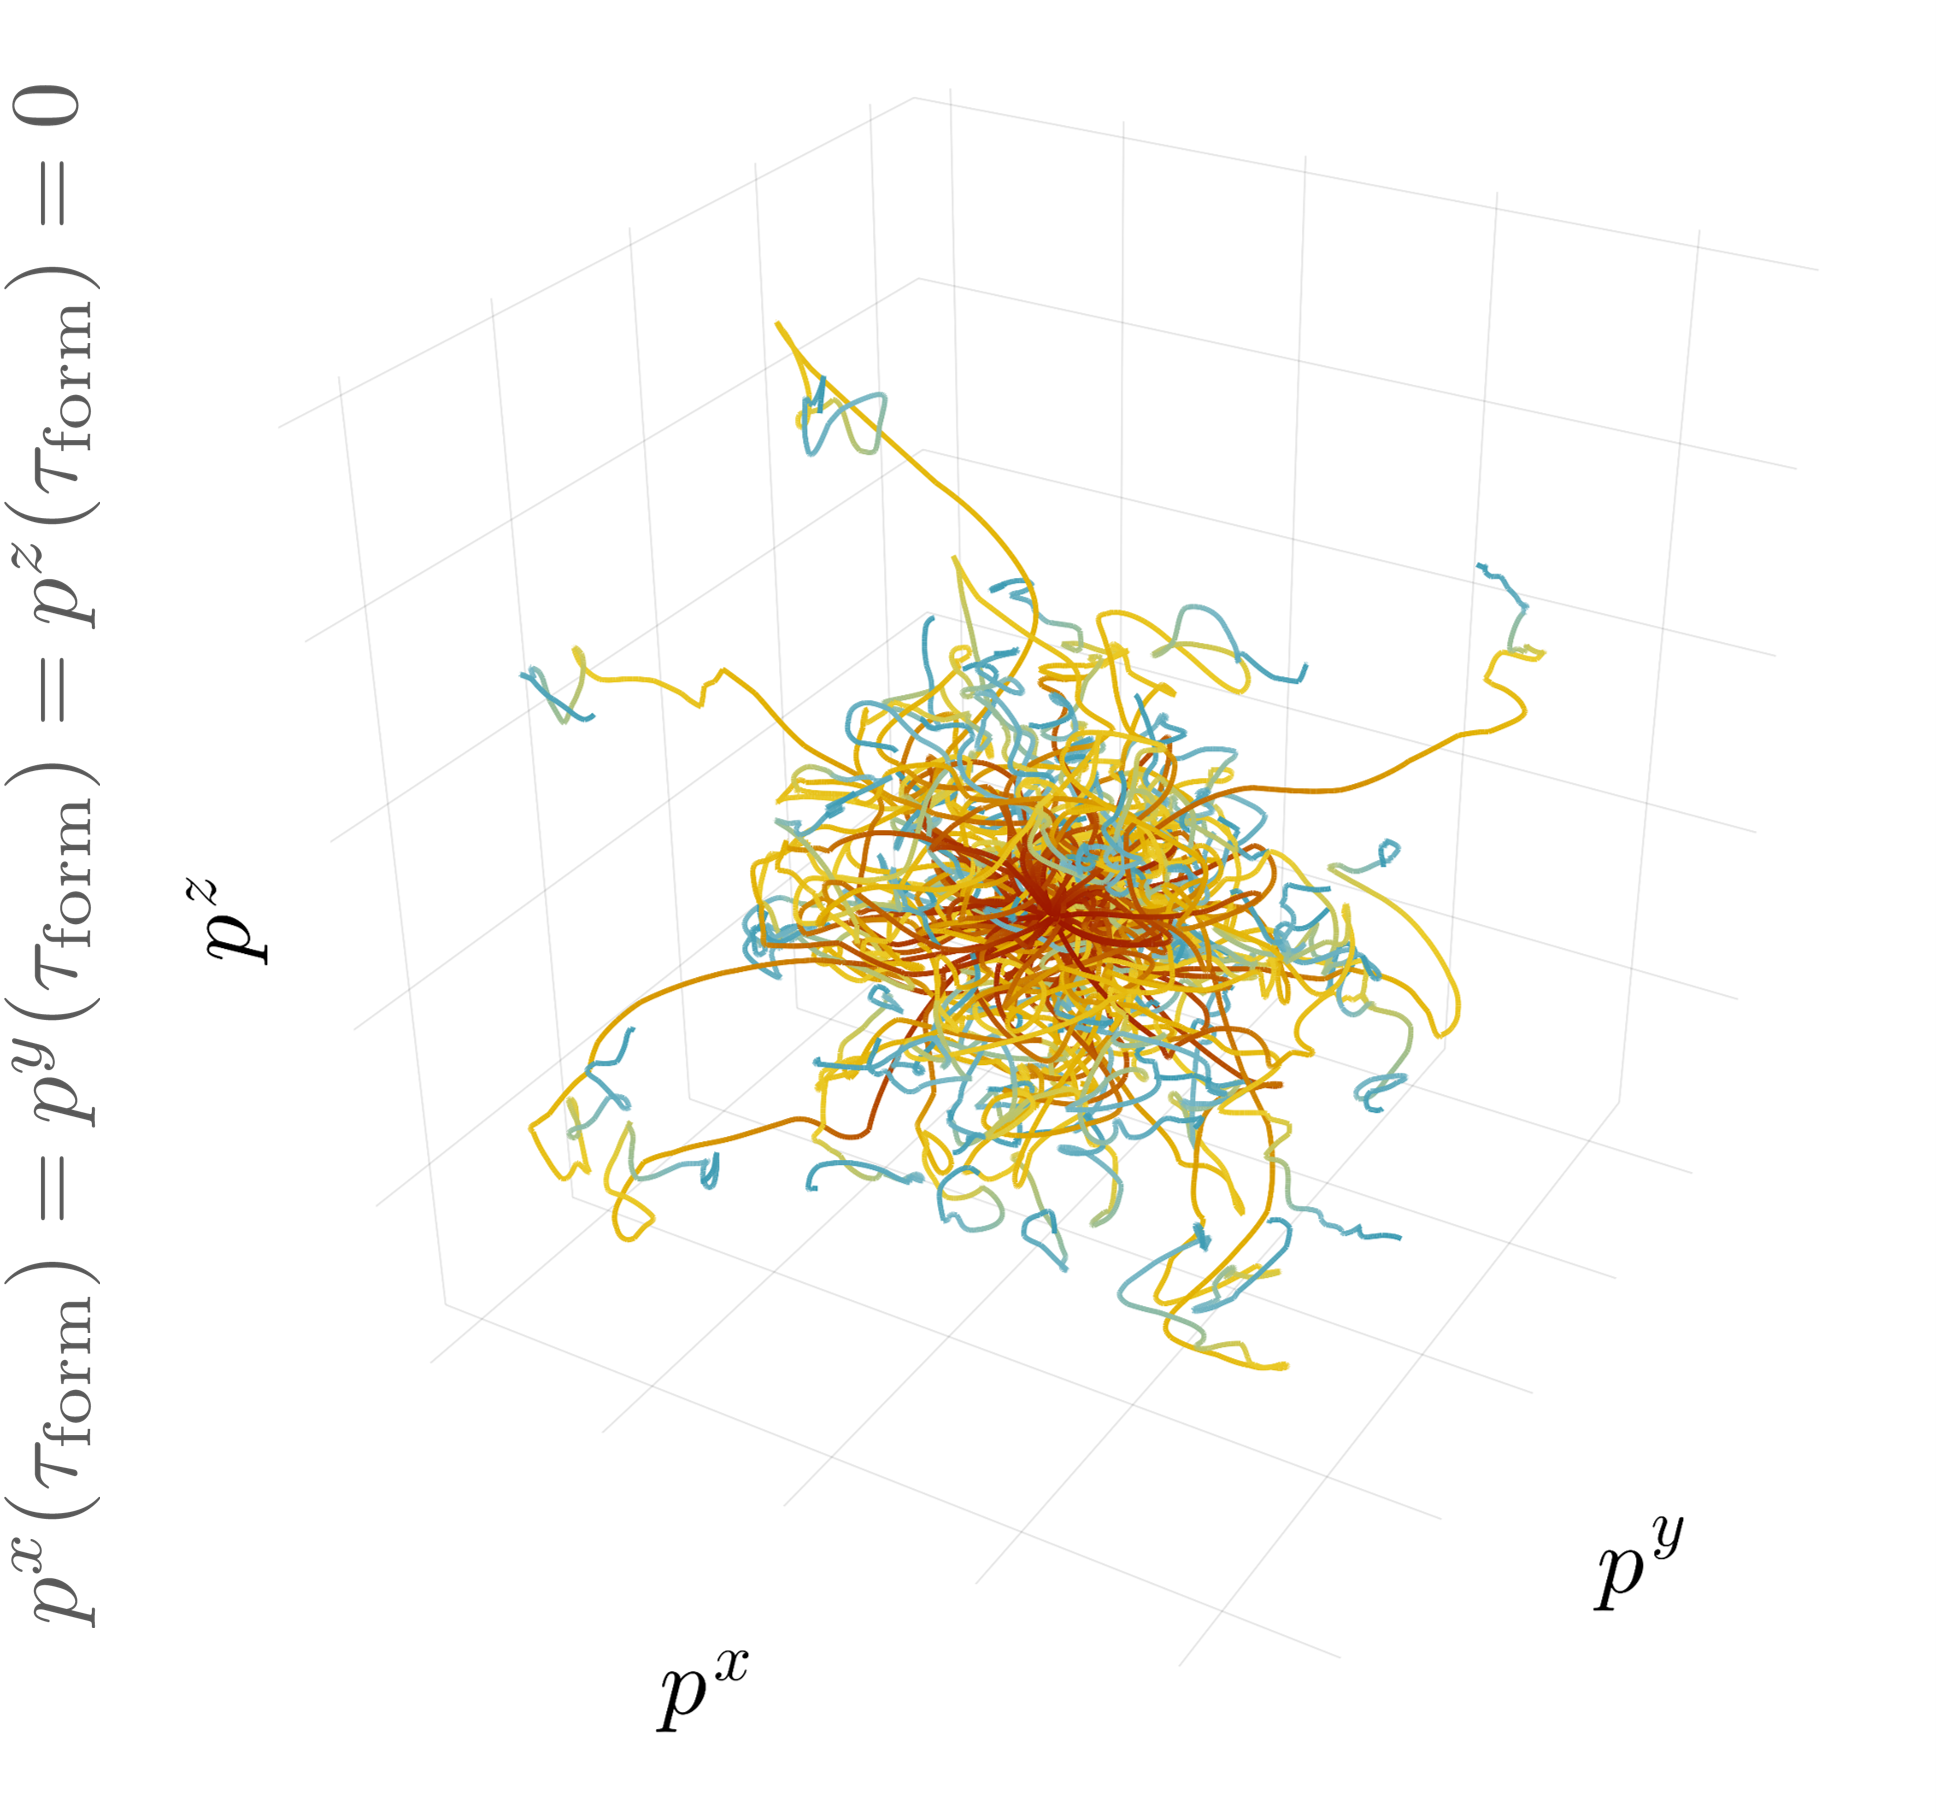
\includegraphics[width=1.1\columnwidth]{images/wong_mom.png}
%             \end{figure}
%             \column{.025\textwidth}
%         \column{.3\textwidth}
%             \begin{center}
%                 Color rotation
%             \end{center}
%             \vspace{-15pt}
%             \begin{figure}[!hbt]
%                 \centering
%                 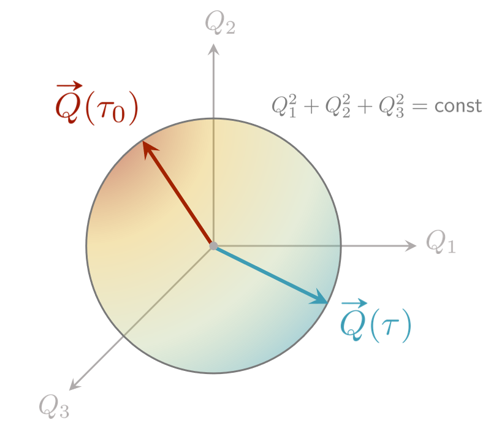
\includegraphics[width=1.05\columnwidth]{images/wong_charge.png}
%             \end{figure}
%             \column{.025\textwidth}
%     \end{columns}
% \end{frame}

% \begin{frame}[noframenumbering]
%     \frametitle{Particles in Yang-Mills fields}
%     % \framesubtitle{Wong's equations of motion} 
%         \begin{itemize}
%             % \setbeamertemplate{itemize item}{\raisebox{0.2em}{\scalebox{0.7}{${\color{ming}\blacktriangleright}$}}}
%             % \item {\large{{\color{ming}Approach}: {\color{ming}numerical trajectories} of classical particles in glasma fields}}
%             \setbeamertemplate{itemize item}{\raisebox{0.2em}{\scalebox{0.7}{${\color{pinky}\blacktriangleright}$}}}
%             \item  {\large{{\color{pinky}Quantities}: averaged over particle trajectories and glasma events}}
%                 \\[10pt]
%                 \begin{itemize}
%                     \item[\raisebox{0.2em}{\scalebox{0.6}{${\color{ming}\blacktriangleright}$}}]   \tikzmarknode{A}{Momentum broadening ${\color{ming}\langle\delta p_i^2\rangle}(\tau)= \langle p_i^2(\tau)-p_i^2(\tau_\mathrm{form})\rangle$} \\[5pt]
%                     \item[\raisebox{0.2em}{\scalebox{0.6}{${\color{ming}\blacktriangleright}$}}] \tikzmarknode{B}{Transport coefficient\footnote{More on transport coefficients in QGP from {\color{jyured}Maria-Lucia}} ${\color{ming}\kappa_i}=\dfrac{\mathrm{d}}{\mathrm{d}\tau}\langle \delta p^2_i(\tau)\rangle$ $\phantom{-p_i^2(\tau_\mathrm{form})abcd}$}\\[5pt]
%                     % \item[\raisebox{0.2em}{\scalebox{0.6}{${\color{pinky}\blacktriangleright}$}}]   \tikzmarknode{B}{Momentum anisotropy ${\color{custompink}\dfrac{\langle\delta p_L^2\rangle}{\langle\delta p_T^2\rangle}}$ $\phantom{= p_i^2(\tau)-p_i^2(\tau_\mathrm{form})abcd}$} \\[5pt]
%                     \item[\raisebox{0.2em}{\scalebox{0.6}{${\color{custompink}\blacktriangleright}$}}] \tikzmarknode{M}{Transverse momentum spectra ${\color{custompink}\dfrac{\mathrm{d}N}{\mathrm{d}p_T}}(\tau)$ using FONLL input $\dfrac{\mathrm{d}N}{\mathrm{d}p_T}(\tau_\mathrm{form})$}\\[5pt]
%                     \item[\raisebox{0.2em}{\scalebox{0.6}{${\color{custompink}\blacktriangleright}$}}] Nuclear modification factor ${\color{custompink}R_{AA}}=\dfrac{\mathrm{d}N^{AA}/\mathrm{d}p_T}{A^2 \mathrm{d}N^{pp}/\mathrm{d}p_T}$ \\[5pt]
%                     \item[\raisebox{0.2em}{\scalebox{0.6}{${\color{custompink}\blacktriangleright}$}}] \tikzmarknode{N}{Two-particle azimuthal correlation ${\color{custompink}\mathcal{C}(\Delta\phi)}= \dfrac{1}{N_\mathrm{pairs}}\dfrac{\mathrm{d}N}{\mathrm{d}\Delta\phi}$ for $Q\overline{Q}$ pairs $\phantom{abcd}$}
%                 \end{itemize}
%         \end{itemize} 

%         \begin{tikzpicture}[overlay,remember picture,
%             BC/.style = {decorate,
%                     decoration={calligraphic brace, amplitude=4pt,
%                     raise=4pt},
%                     thick,
%                     pen colour=ming}
%                              ]
%             \path[BC]   (A.north -| B.east) -- node[right=8pt] {\color{ming}theoretical} (B.south east);
%         \end{tikzpicture}
%         \begin{tikzpicture}[overlay,remember picture,
%             NO/.style = {decorate,
%                     decoration={calligraphic brace, amplitude=4pt,
%                     raise=4pt},
%                     thick,
%                     pen colour=custompink}
%                              ]
%             \path[NO]   (M.north -| N.east) -- node[right=8pt] {\color{custompink}observables\footnote{More on HF observables from {\color{jyured} Mattia}}} (N.south east);
%         \end{tikzpicture}
% \end{frame}

% % \begin{frame}
% %     \begin{itemize}
% % \item   a: there is some \tikzmarknode{A}{content}
% % \item   b: in this item is some longer \tikzmarknode{B}{content}
% % \item   last item 
% %     \end{itemize}
% % \begin{tikzpicture}[overlay,remember picture,
% % BC/.style = {decorate,
% %         decoration={calligraphic brace, amplitude=4pt,
% %         raise=4pt},
% %         very thick,
% %         pen colour=red}
% %                  ]
% % \path[BC]   (A.north -| B.east) -- node[right=8pt] {$\Longrightarrow d$} (B.south east);
% % \end{tikzpicture}
% % \end{frame}


% \setbeamertemplate{itemize item}{\raisebox{0.2em}{\scalebox{0.7}{${\color{customblue}\blacktriangleright}$}}}

% % \begin{frame}[t]
% %     \frametitle{Numerical trajectories results}
% %     \begin{center}
% %         \begin{tikzpicture}[xscale=1]%[scale=0.9, every node/.style={scale=0.6}]
% %             % \draw[line width=2mm,-latex,red!20] (-0.2,0) -- (9,0);
% %             \draw[line width=0.5mm,-latex,customblue!20] (-0.2,0) -- (8.5+0.2,0);
% %             \foreach \X [evaluate=\X as \Y using int(\X-2017),count=\Z] in {2018, 2019, 2021, 2022, 2024}
% %             {
% %             % \draw[highlight on=<\Z>] ({\Y-0.2},-0.5) -- ({\Y+0.2},-0.5) -- (\Y,-0.1) -- cycle;
% %             \draw[highlight on=<\Z>] (\Y,0) circle[radius=2.5pt];
% %             % \node[circle, highlight on=<\Z>,inner sep=2pt,color=customblue] at (\Y,0) {};
% %             \node[anchor=south,highlight on=<\Z>,fill=white,rotate=45,anchor=south
% %             west,inner sep=0pt] at (\Y,0.2) {\X};
% %             }
% %         \end{tikzpicture}
% %     \end{center}
% %     \vspace{-10pt}
% %     \begin{columns}[onlytextwidth,t]
% %         \column{.02\textwidth}
% %        \column{.44\textwidth}
% %        \begin{figure}
% %             \centering
% %             \captionsetup{justification=centering}
% %             \only<1>{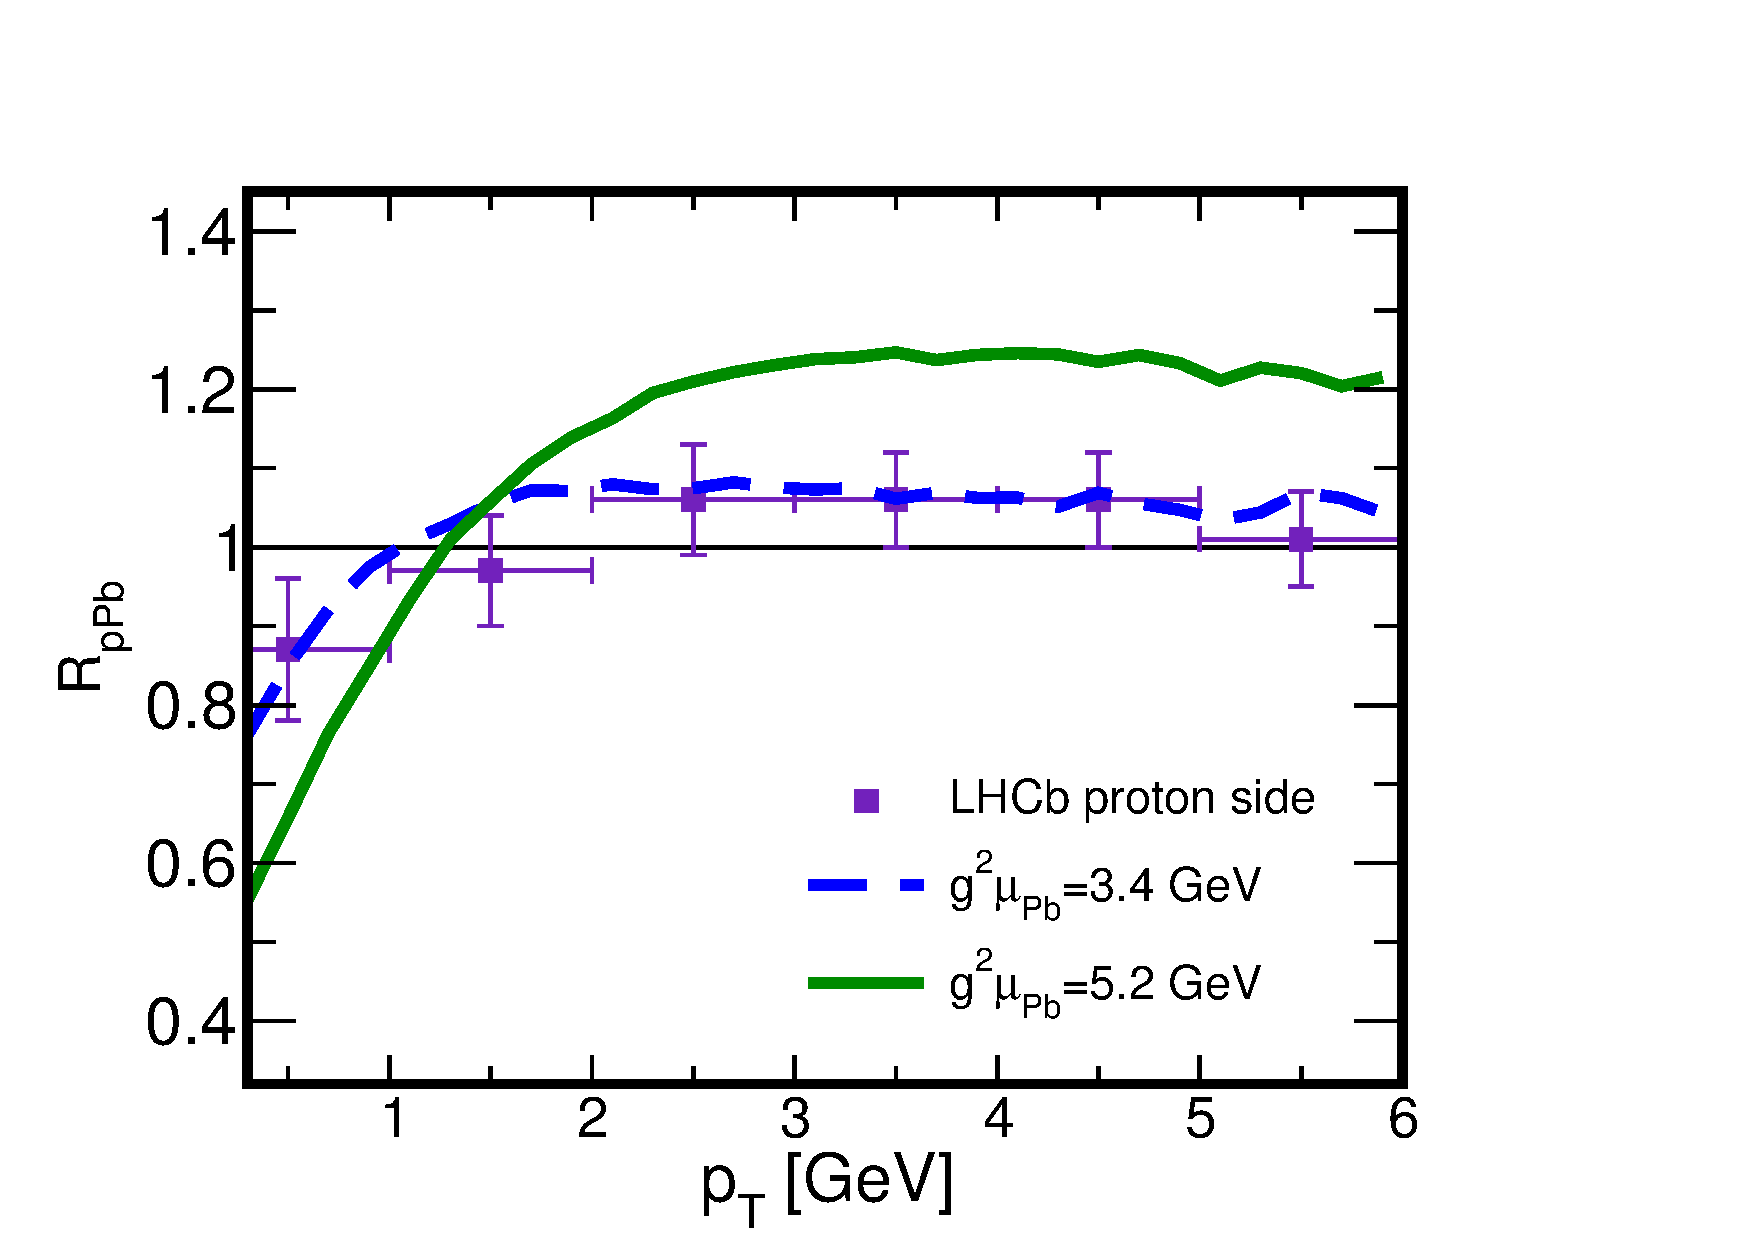
\includegraphics[width=\textwidth]{images/pPb_RpPb_FRAGME_new_2.pdf}}
% %             \only<2>{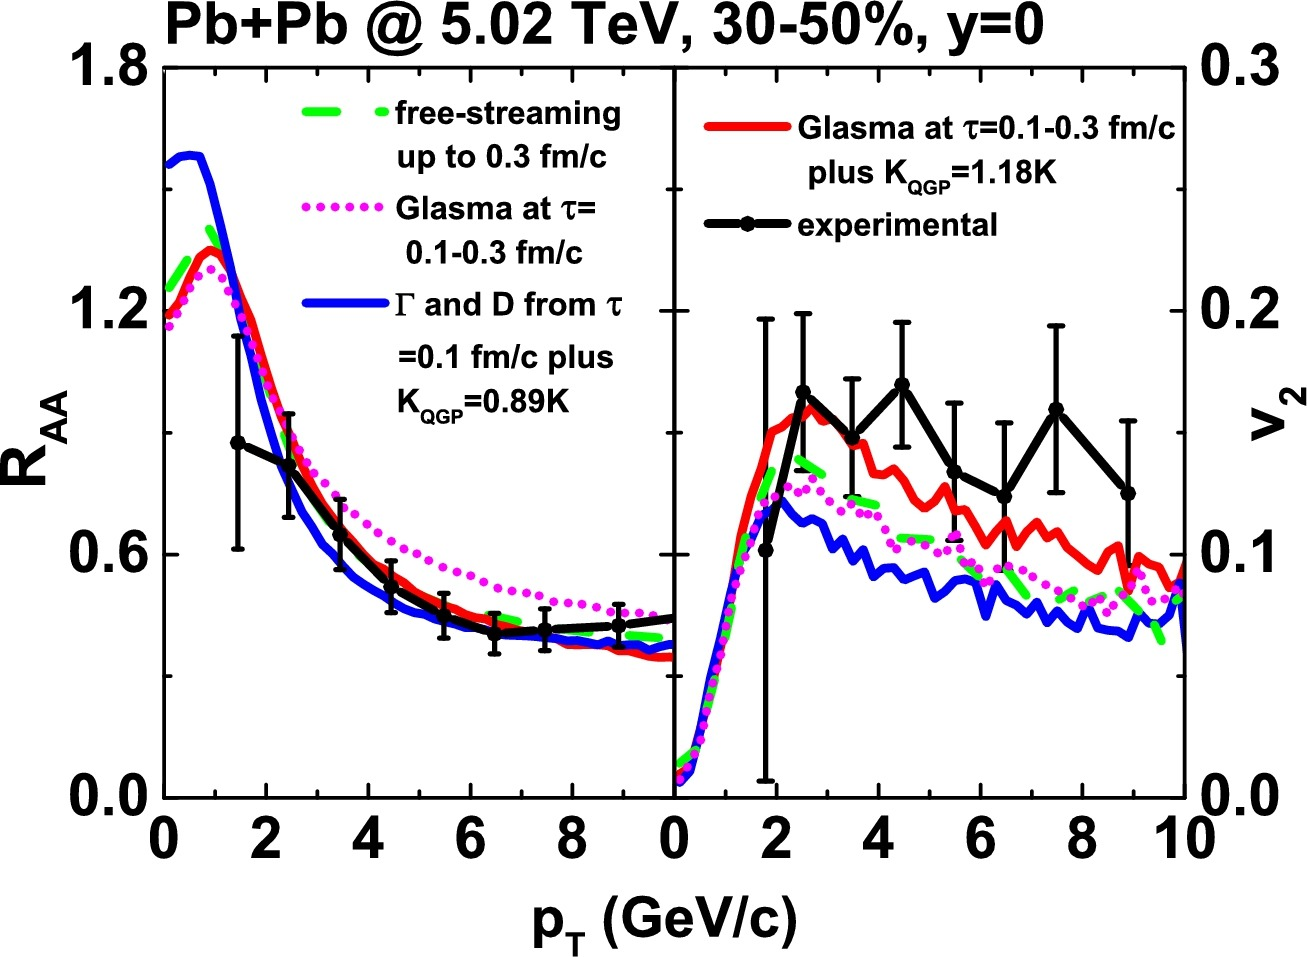
\includegraphics[width=0.95\textwidth]{images/1-s2.0-S0370269319306550-gr003_lrg.jpg}}
% %             \only<3>{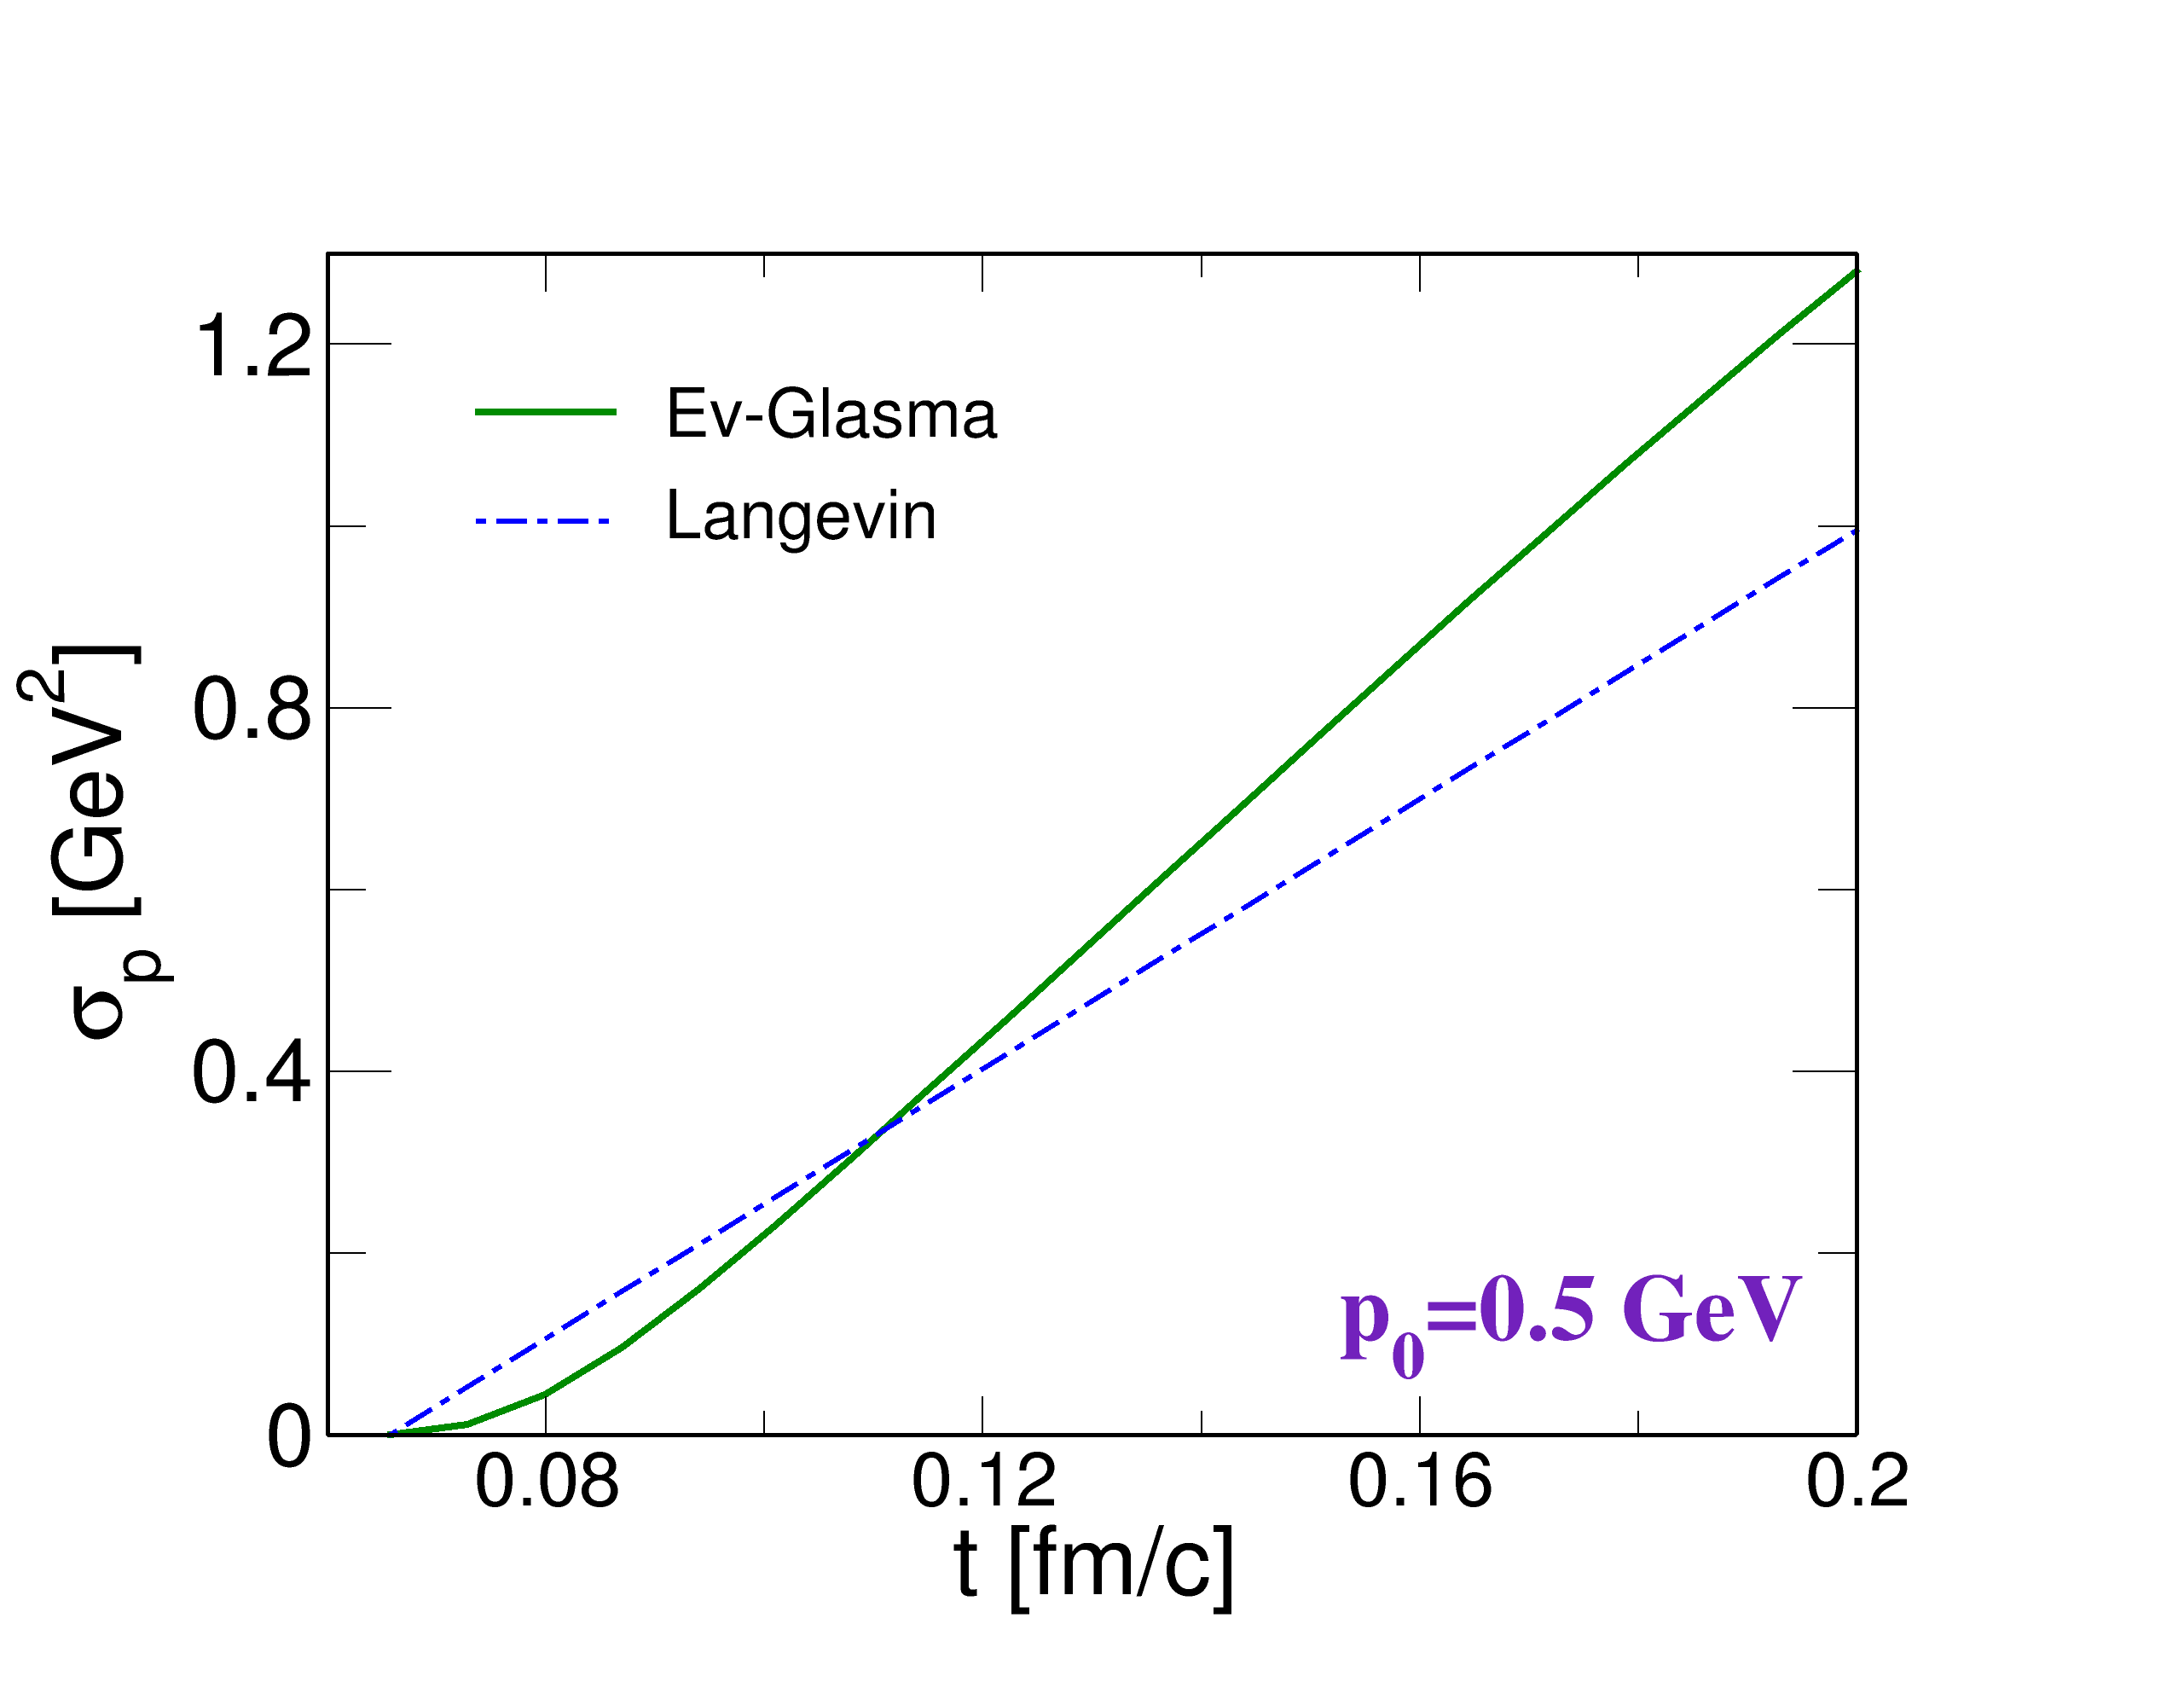
\includegraphics[width=0.95\textwidth]{images/zoom_02fm_langevin.png}}
% %             \only<4>{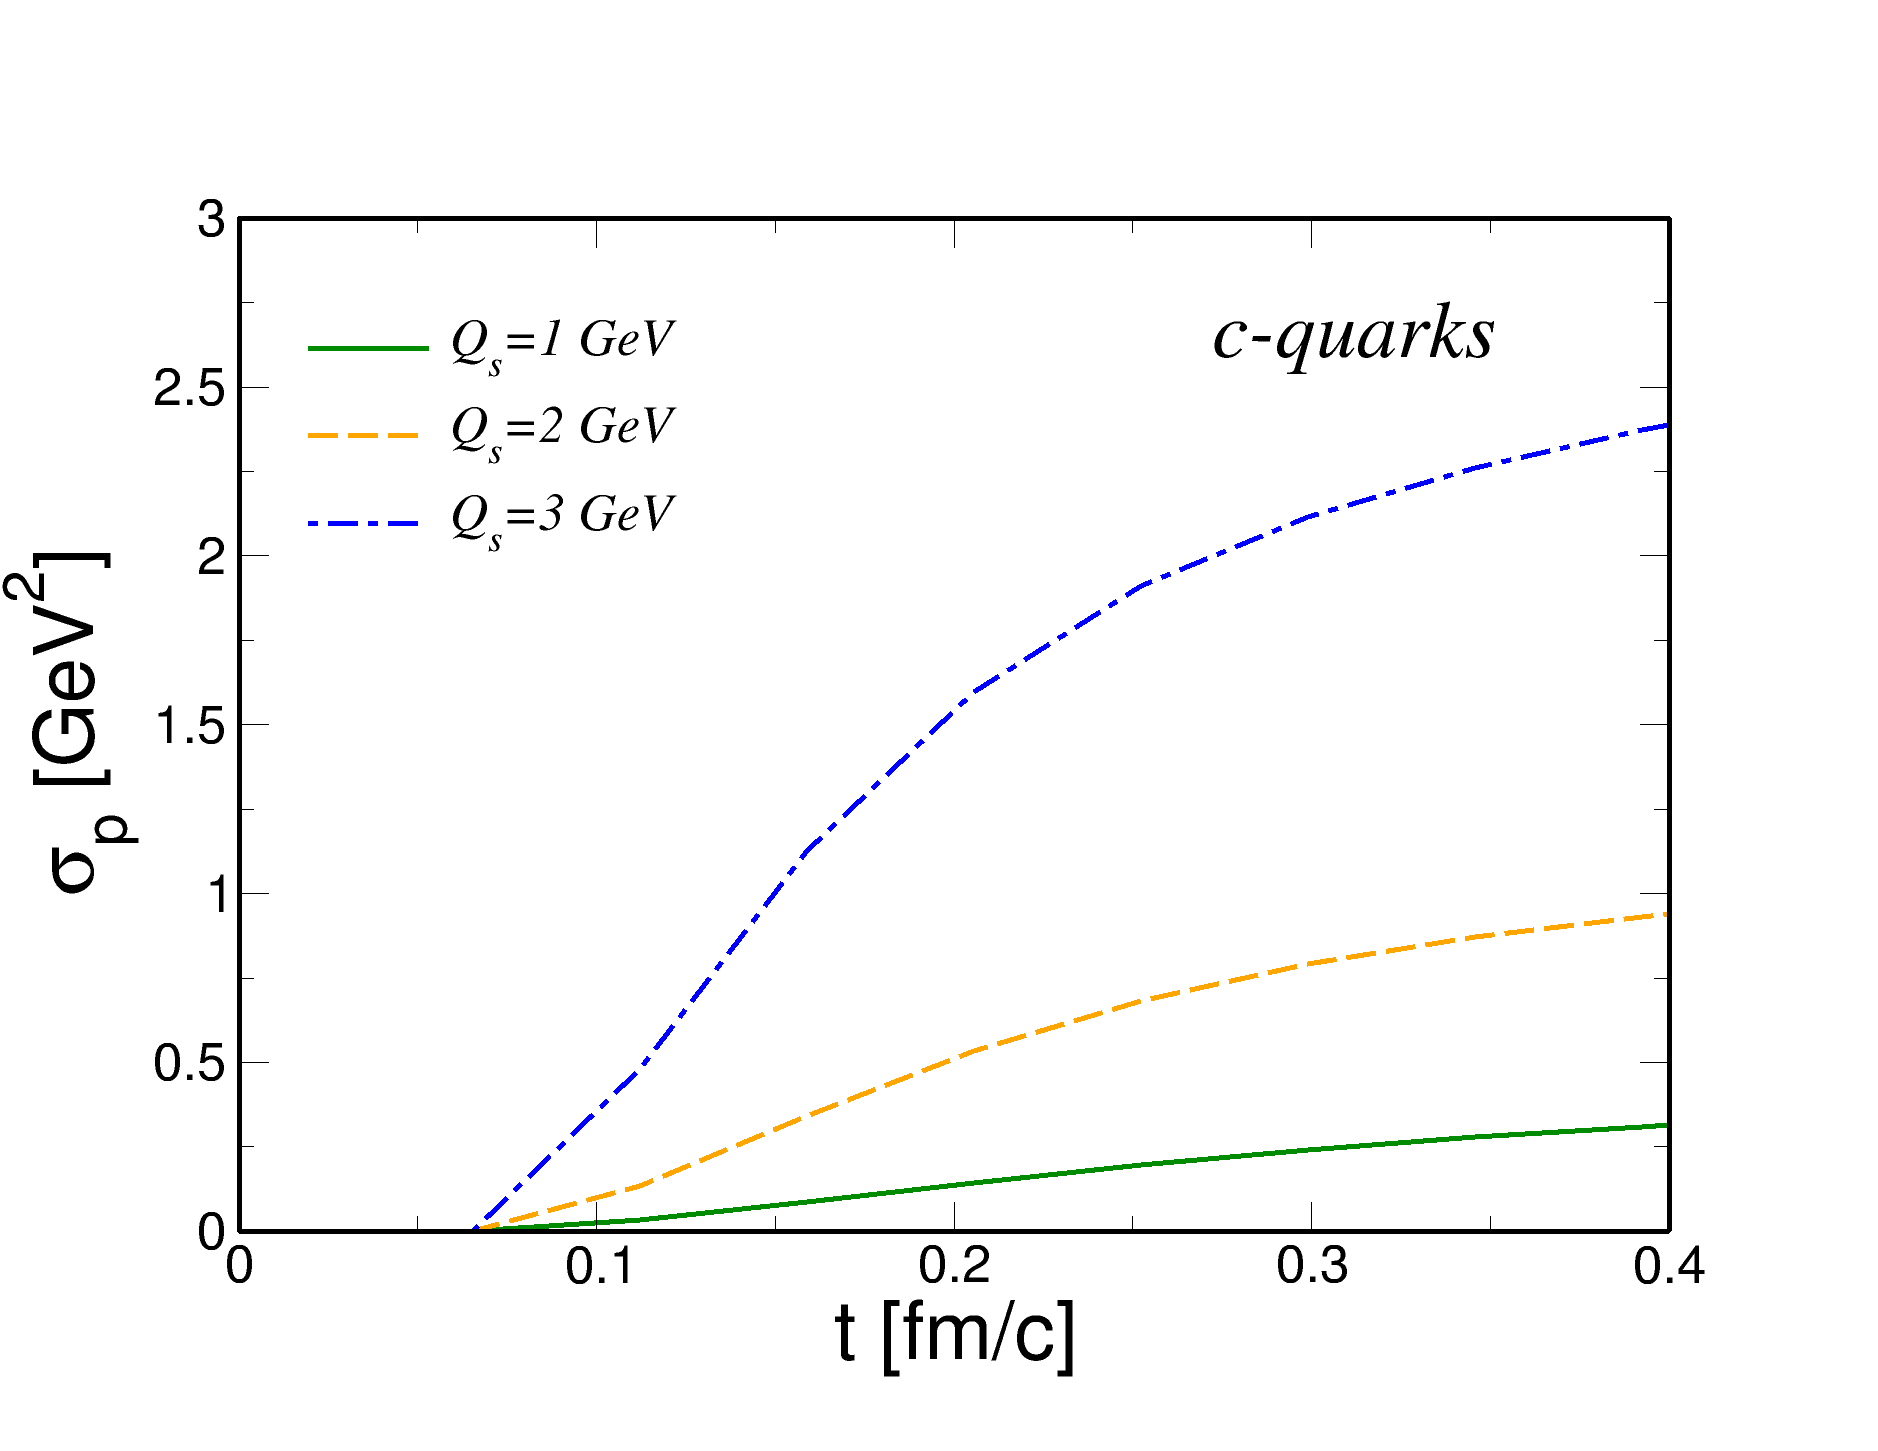
\includegraphics[width=0.95\textwidth]{images/sigmap_charm_expanding_04.png}}
% %             \only<5>{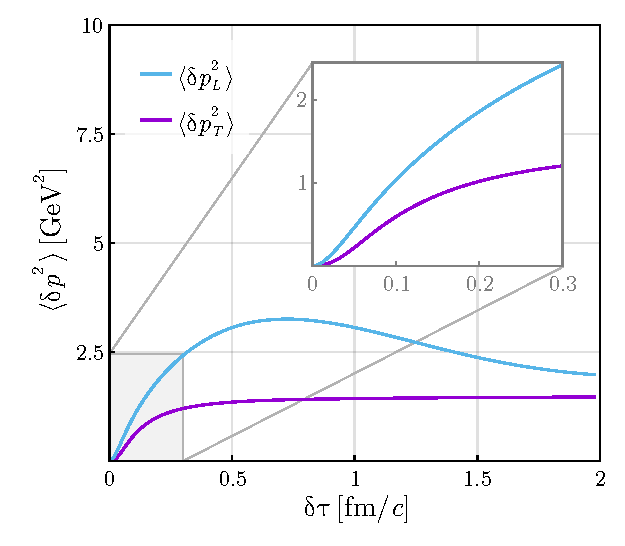
\includegraphics[width=0.9\textwidth]{images/beauty_early_behaviour_mom_broad.pdf}}
% %             \only<6>{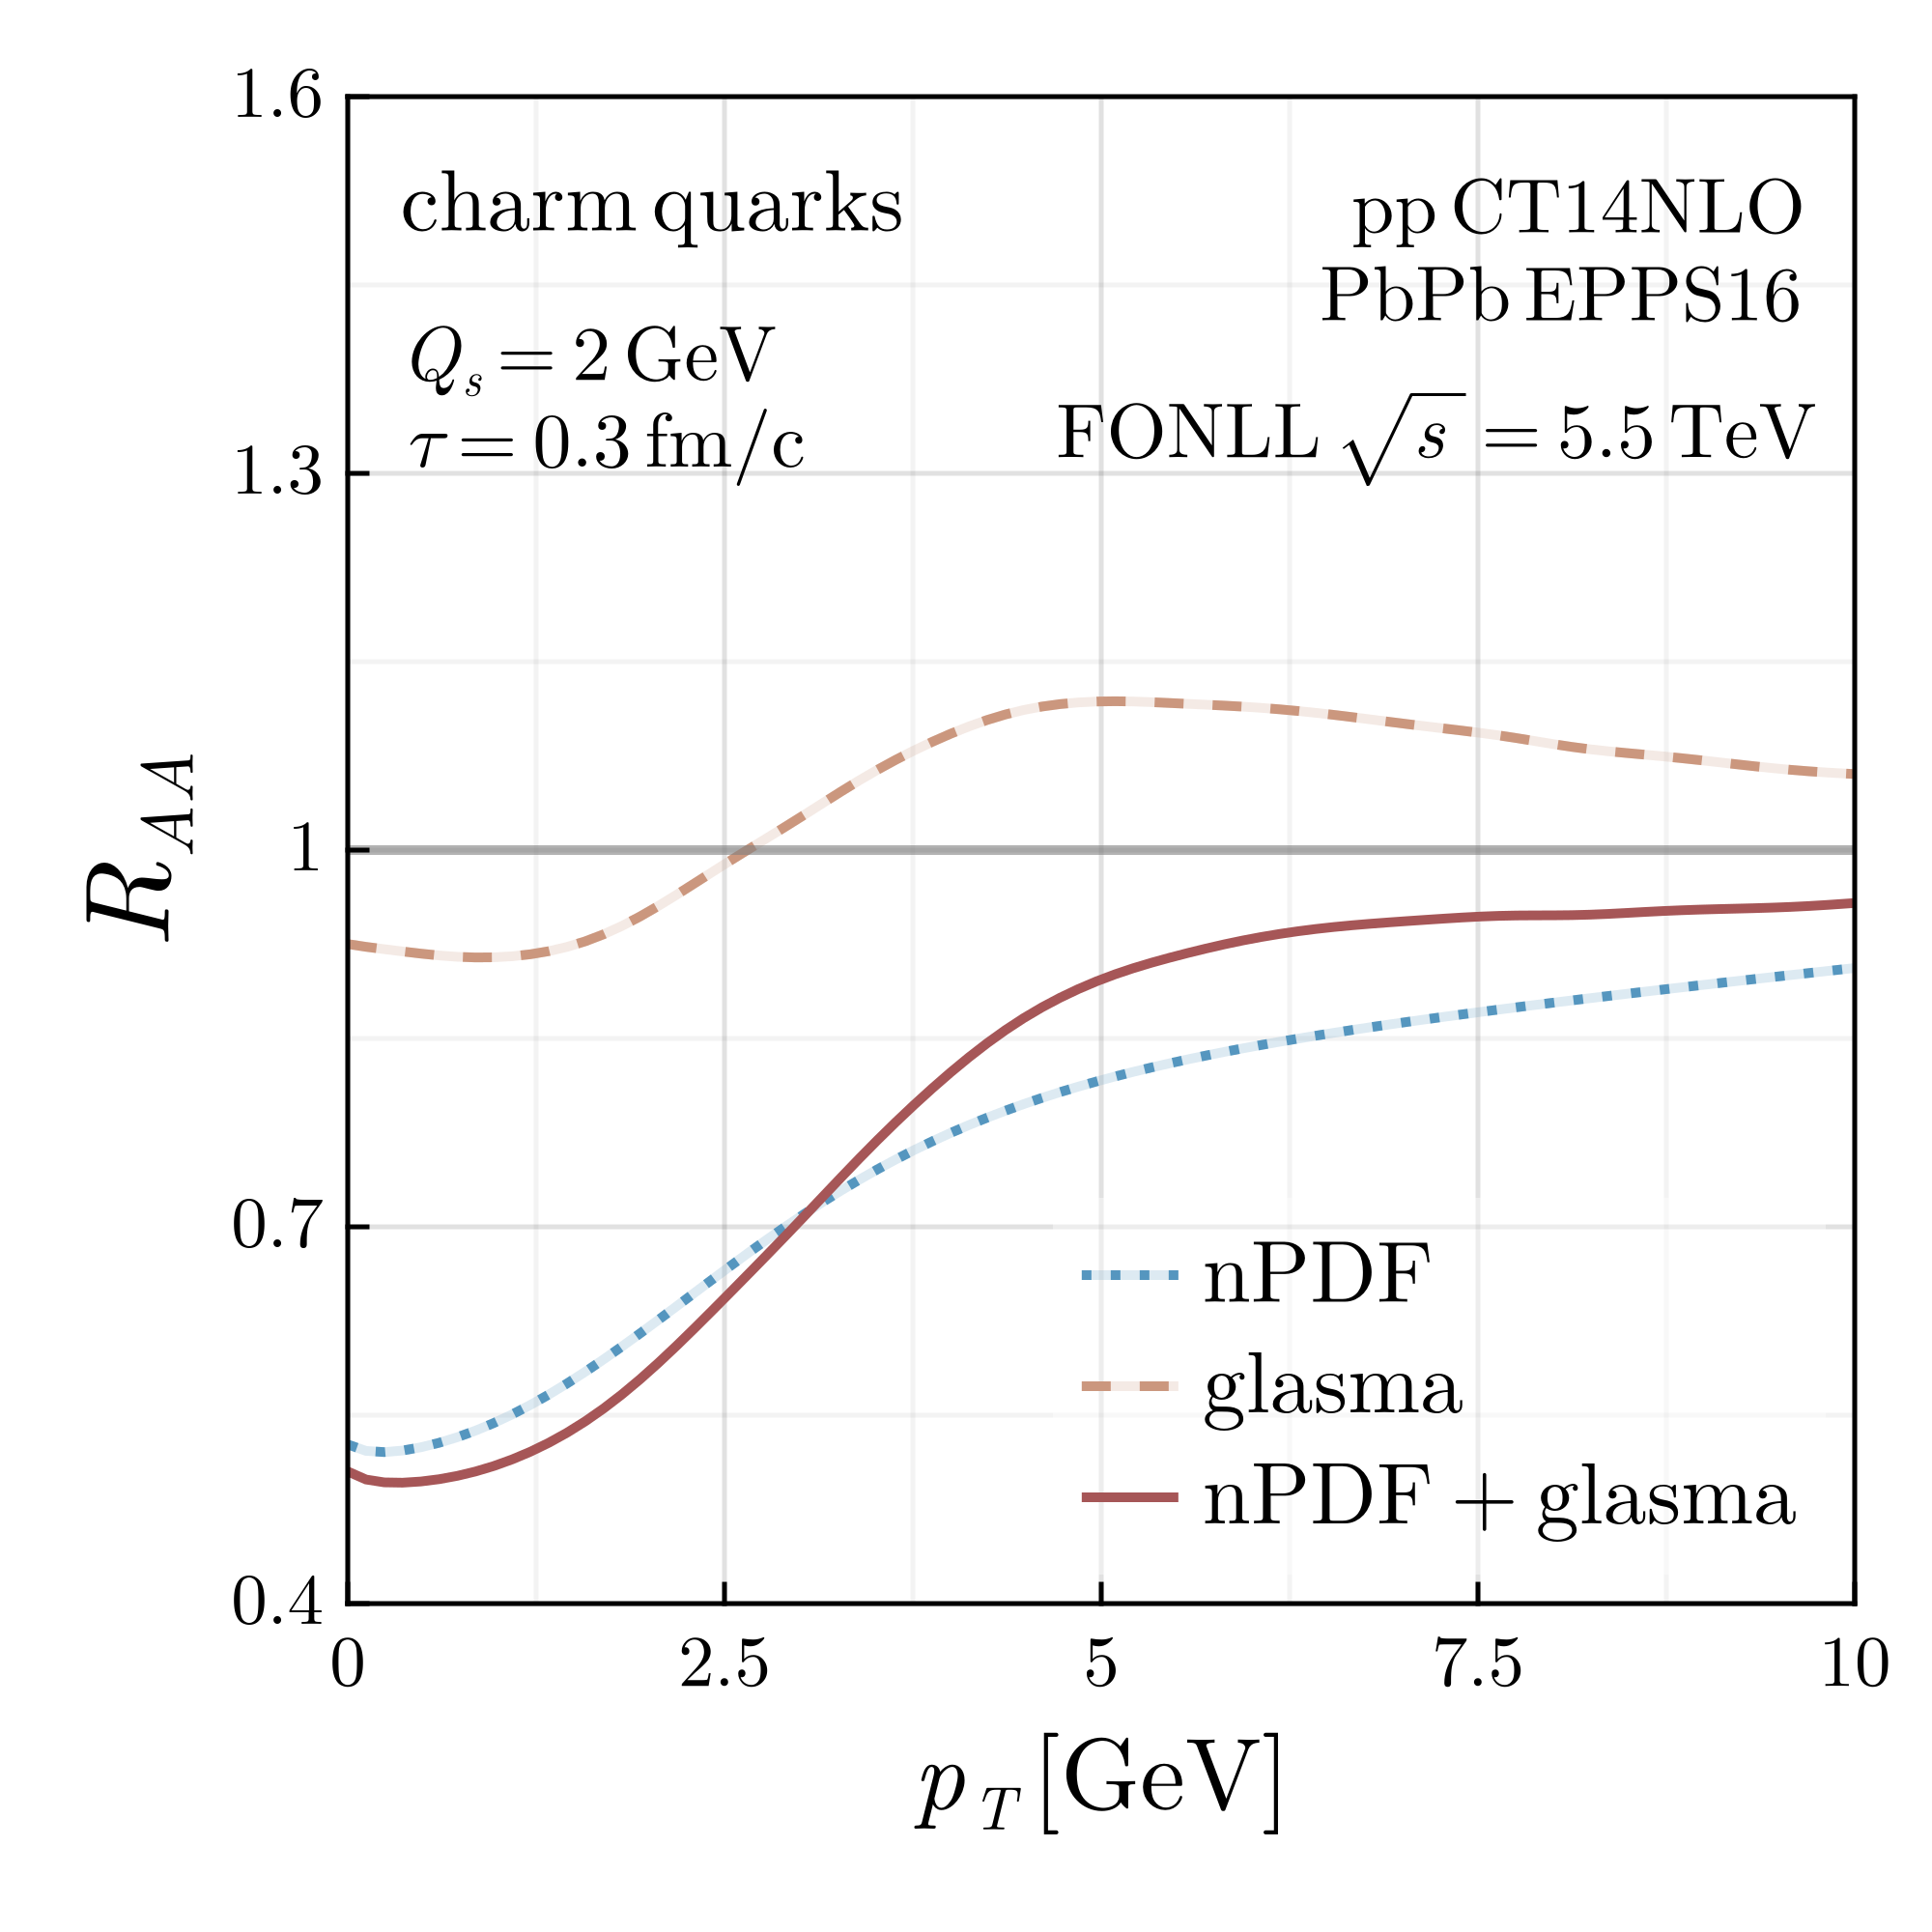
\includegraphics[width=0.8\textwidth]{images/clean_raa_tau_0.3_charm_quark_Qs_2.0_fonll_pdf_vs_npdf_v3.png}}
% %             \only<7>{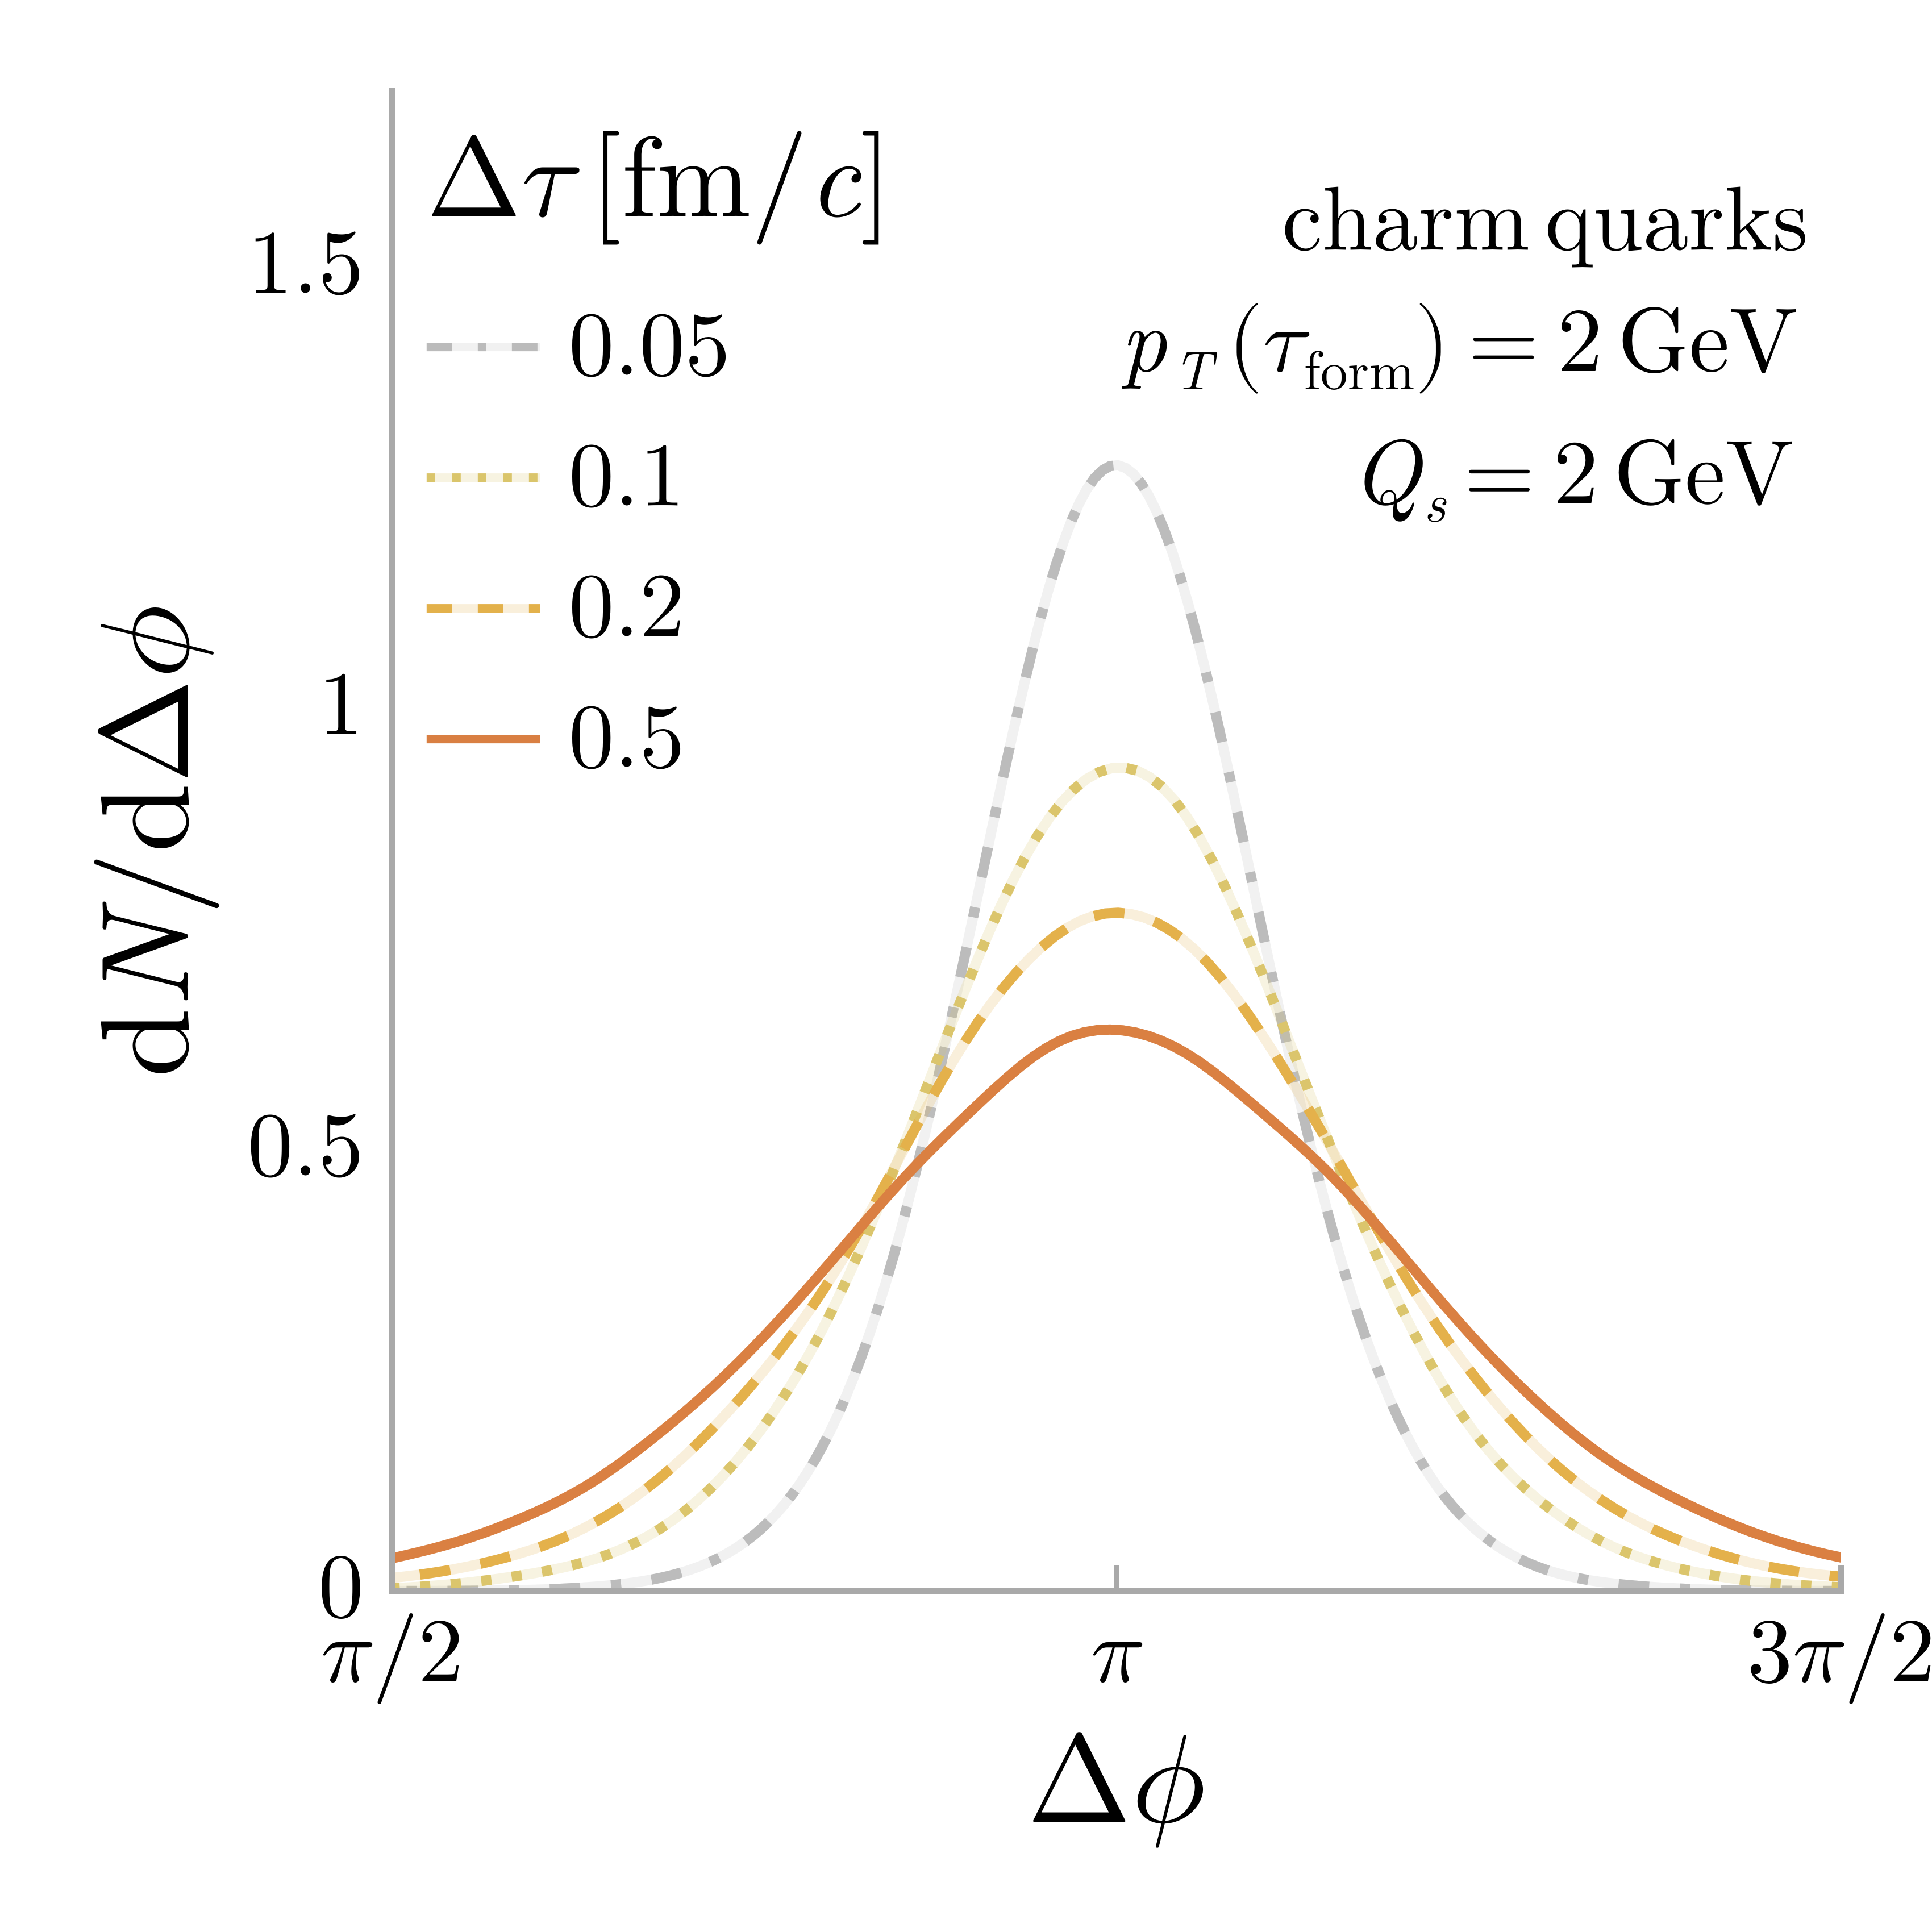
\includegraphics[width=0.8\textwidth]{images/final_dNdphi_tau_dep_charm_v2.png}}
% %         \end{figure}
% %         \column{.02\textwidth}
% %         \column{.5\textwidth}
% %         % \vspace{0.2cm}
% %         \begin{center}
% %             \begin{itemize}
% %                 \item<1> $R_{pA}$ for D-mesons\only<1>{\footnotemark \\[5pt] {\color{lightgray}\footnotesize FONLL input + fragmentation\\
% %                 SU(2) glasma, static box}}
% %                 \item<2> Hybrid $R_{AA}$ and $v_2$\only<2>{\footnotemark \\[5pt] {\color{lightgray}\footnotesize Compared with Fokker-Planck diffusion\\
% %                 SU(2) glasma, static box}}
% %                 \only<3>{\item Momentum variance $\sigma_p$\footnotemark \\[5pt] {\color{lightgray}\footnotesize Compared with Langevin diffusion\\
% %                 SU(2) glasma, static box}}
% %                 \item<4> Momentum variance $\sigma_p$\only<4>{\footnotemark \\[5pt] {\color{lightgray}\footnotesize SU(2) glasma, longitudinal expansion}}
% %                 \item<5> Momentum broadening $\langle \delta p^2\rangle$\only<5>{\footnotemark}\\
% %                 Transport coefficient $\kappa$\only<5>{\footnotemark \\[5pt] {\color{lightgray}\footnotesize SU(3) glasma, CPIC particle solver}}
% %                 \item<6> $R_{AA}$ with nPDF effects
% %                 \item<7> Azimuthal decorrelation $\mathcal{C}(\Delta\phi)$ \only<7>{\\[5pt] {\color{lightgray}\footnotesize $Q\overline{Q}$ pairs evolve in glasma}}
% %             \end{itemize}
% %         \end{center}
% %         \column{.02\textwidth}
% %     \end{columns}
% %     \only<1>{\footnotetext{\scriptsize Ruggieri, Das \href{https://journals.aps.org/prd/abstract/10.1103/PhysRevD.98.094024}{{\color{customblue}\texttt{[Phys.Rev.D98(2018)]}}}}}
% %     \only<2>{\footnotetext{\scriptsize Sun, Coci, Das, Plumari, Ruggieri, Greco \href{https://doi.org/10.1016/j.physletb.2019.134933}{{\color{customblue}\texttt{[Phys.Lett.B798(2019)]}}}}}
% %     \only<3>{\footnotetext{\scriptsize Liu, Das, Greco, Ruggieri \href{https://journals.aps.org/prd/abstract/10.1103/PhysRevD.103.034029}{{\color{customblue}\texttt{[Phys.Rev.D103(2021)]}}}}}
% %     \only<4>{\footnotetext{\scriptsize Khowal, Das, Oliva, Ruggieri \href{https://link.springer.com/article/10.1140/epjp/s13360-022-02517-w}{{\color{customblue}\texttt{[Eur.Phys.J.Plus137(2022)]}}}}}
% %     \only<5>{\footnotetext{\scriptsize Avramescu, Băran, Greco, Ipp, Müller, Ruggieri  \href{https://journals.aps.org/prd/abstract/10.1103/PhysRevD.107.114021}{{\color{customblue}\texttt{[Phys.Rev.D107(2023)]}}}}}
% %     % only<2>{\footnotetext{\scriptsize Sun, Coci, Das, Plumari, Ruggieri, Greco  \href{https://doi.org/10.1016/j.physletb.2019.134933}{{\color{customblue}\texttt{[Phys.Lett.B798(2019)]}}}}}
% % \end{frame}

% \begin{frame}[t]
%     \frametitle{Numerical trajectories results}
%     \begin{center}
%         \begin{tikzpicture}[xscale=1]%[scale=0.9, every node/.style={scale=0.6}]
%             % \draw[line width=2mm,-latex,red!20] (-0.2,0) -- (9,0);
%             \draw[line width=0.5mm,-latex,customblue!20] (-0.2,0) -- (8.5+0.2,0);
%             \foreach \X [evaluate=\X as \Y using int(\X-2017),count=\Z] in {2018, 2019, 2021, 2022, 2024}
%             {
%             % \draw[highlight on=<\Z>] ({\Y-0.2},-0.5) -- ({\Y+0.2},-0.5) -- (\Y,-0.1) -- cycle;
%             \draw[highlight on=<\Z>] (\Y,0) circle[radius=2.5pt];
%             % \node[circle, highlight on=<\Z>,inner sep=2pt,color=customblue] at (\Y,0) {};
%             \node[anchor=south,highlight on=<\Z>,fill=white,rotate=45,anchor=south
%             west,inner sep=0pt] at (\Y,0.2) {\X};
%             }
%         \end{tikzpicture}
%     \end{center}
%     \vspace{-10pt}
%     \begin{columns}[onlytextwidth,t]
%         \column{.02\textwidth}
%        \column{.44\textwidth}
%        \begin{figure}
%             \centering
%             \captionsetup{justification=centering}
%             \only<1>{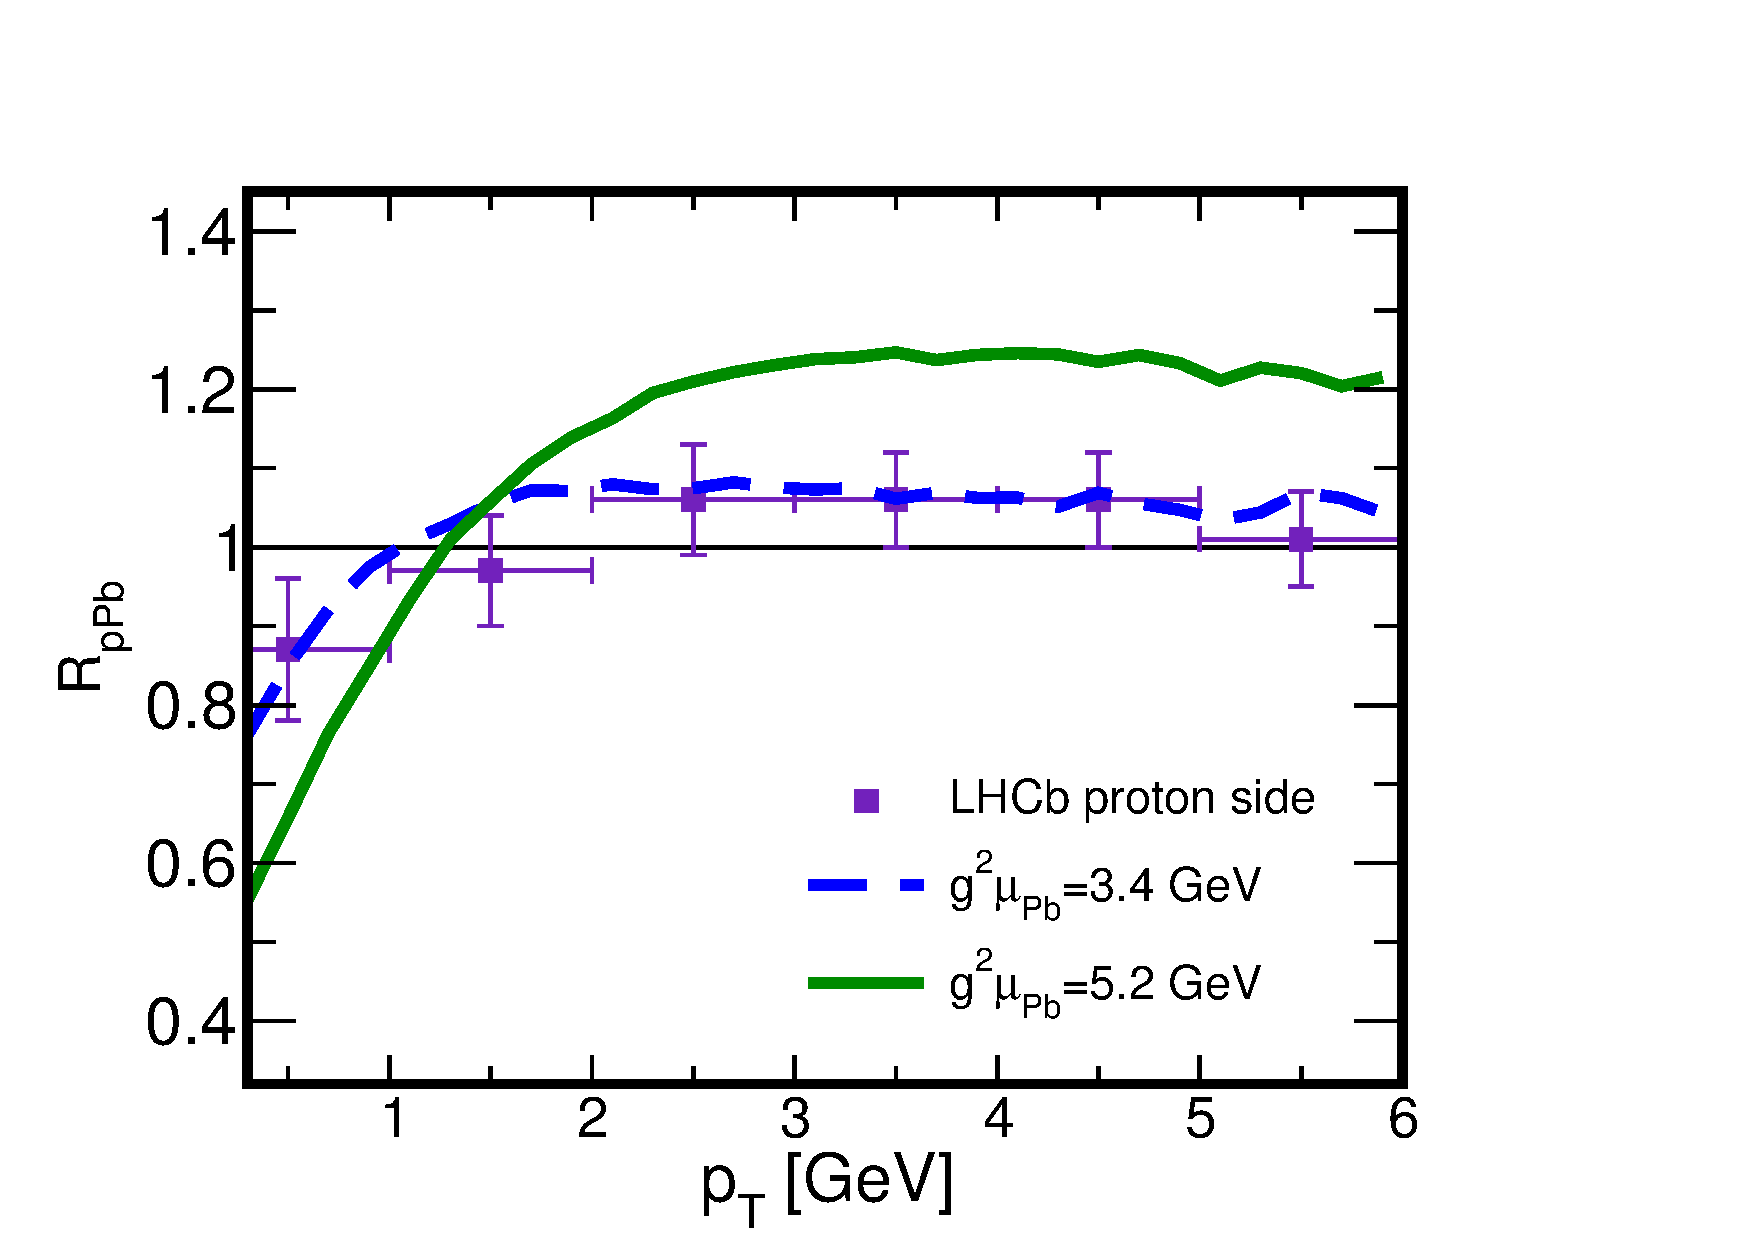
\includegraphics[width=\textwidth]{images/pPb_RpPb_FRAGME_new_2.pdf}}
%             \only<2>{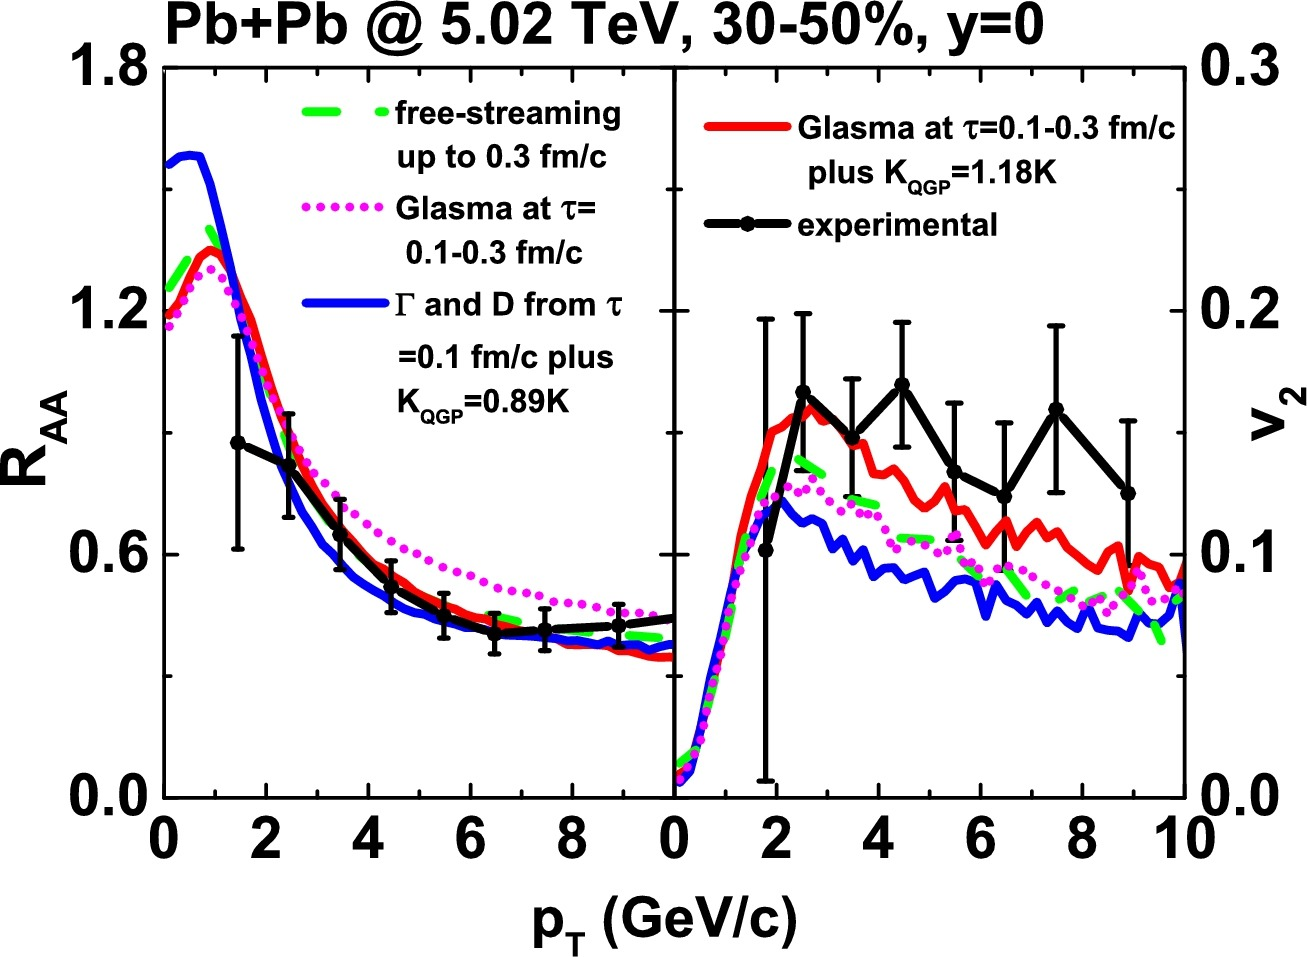
\includegraphics[width=0.95\textwidth]{images/1-s2.0-S0370269319306550-gr003_lrg.jpg}}
%             \only<3>{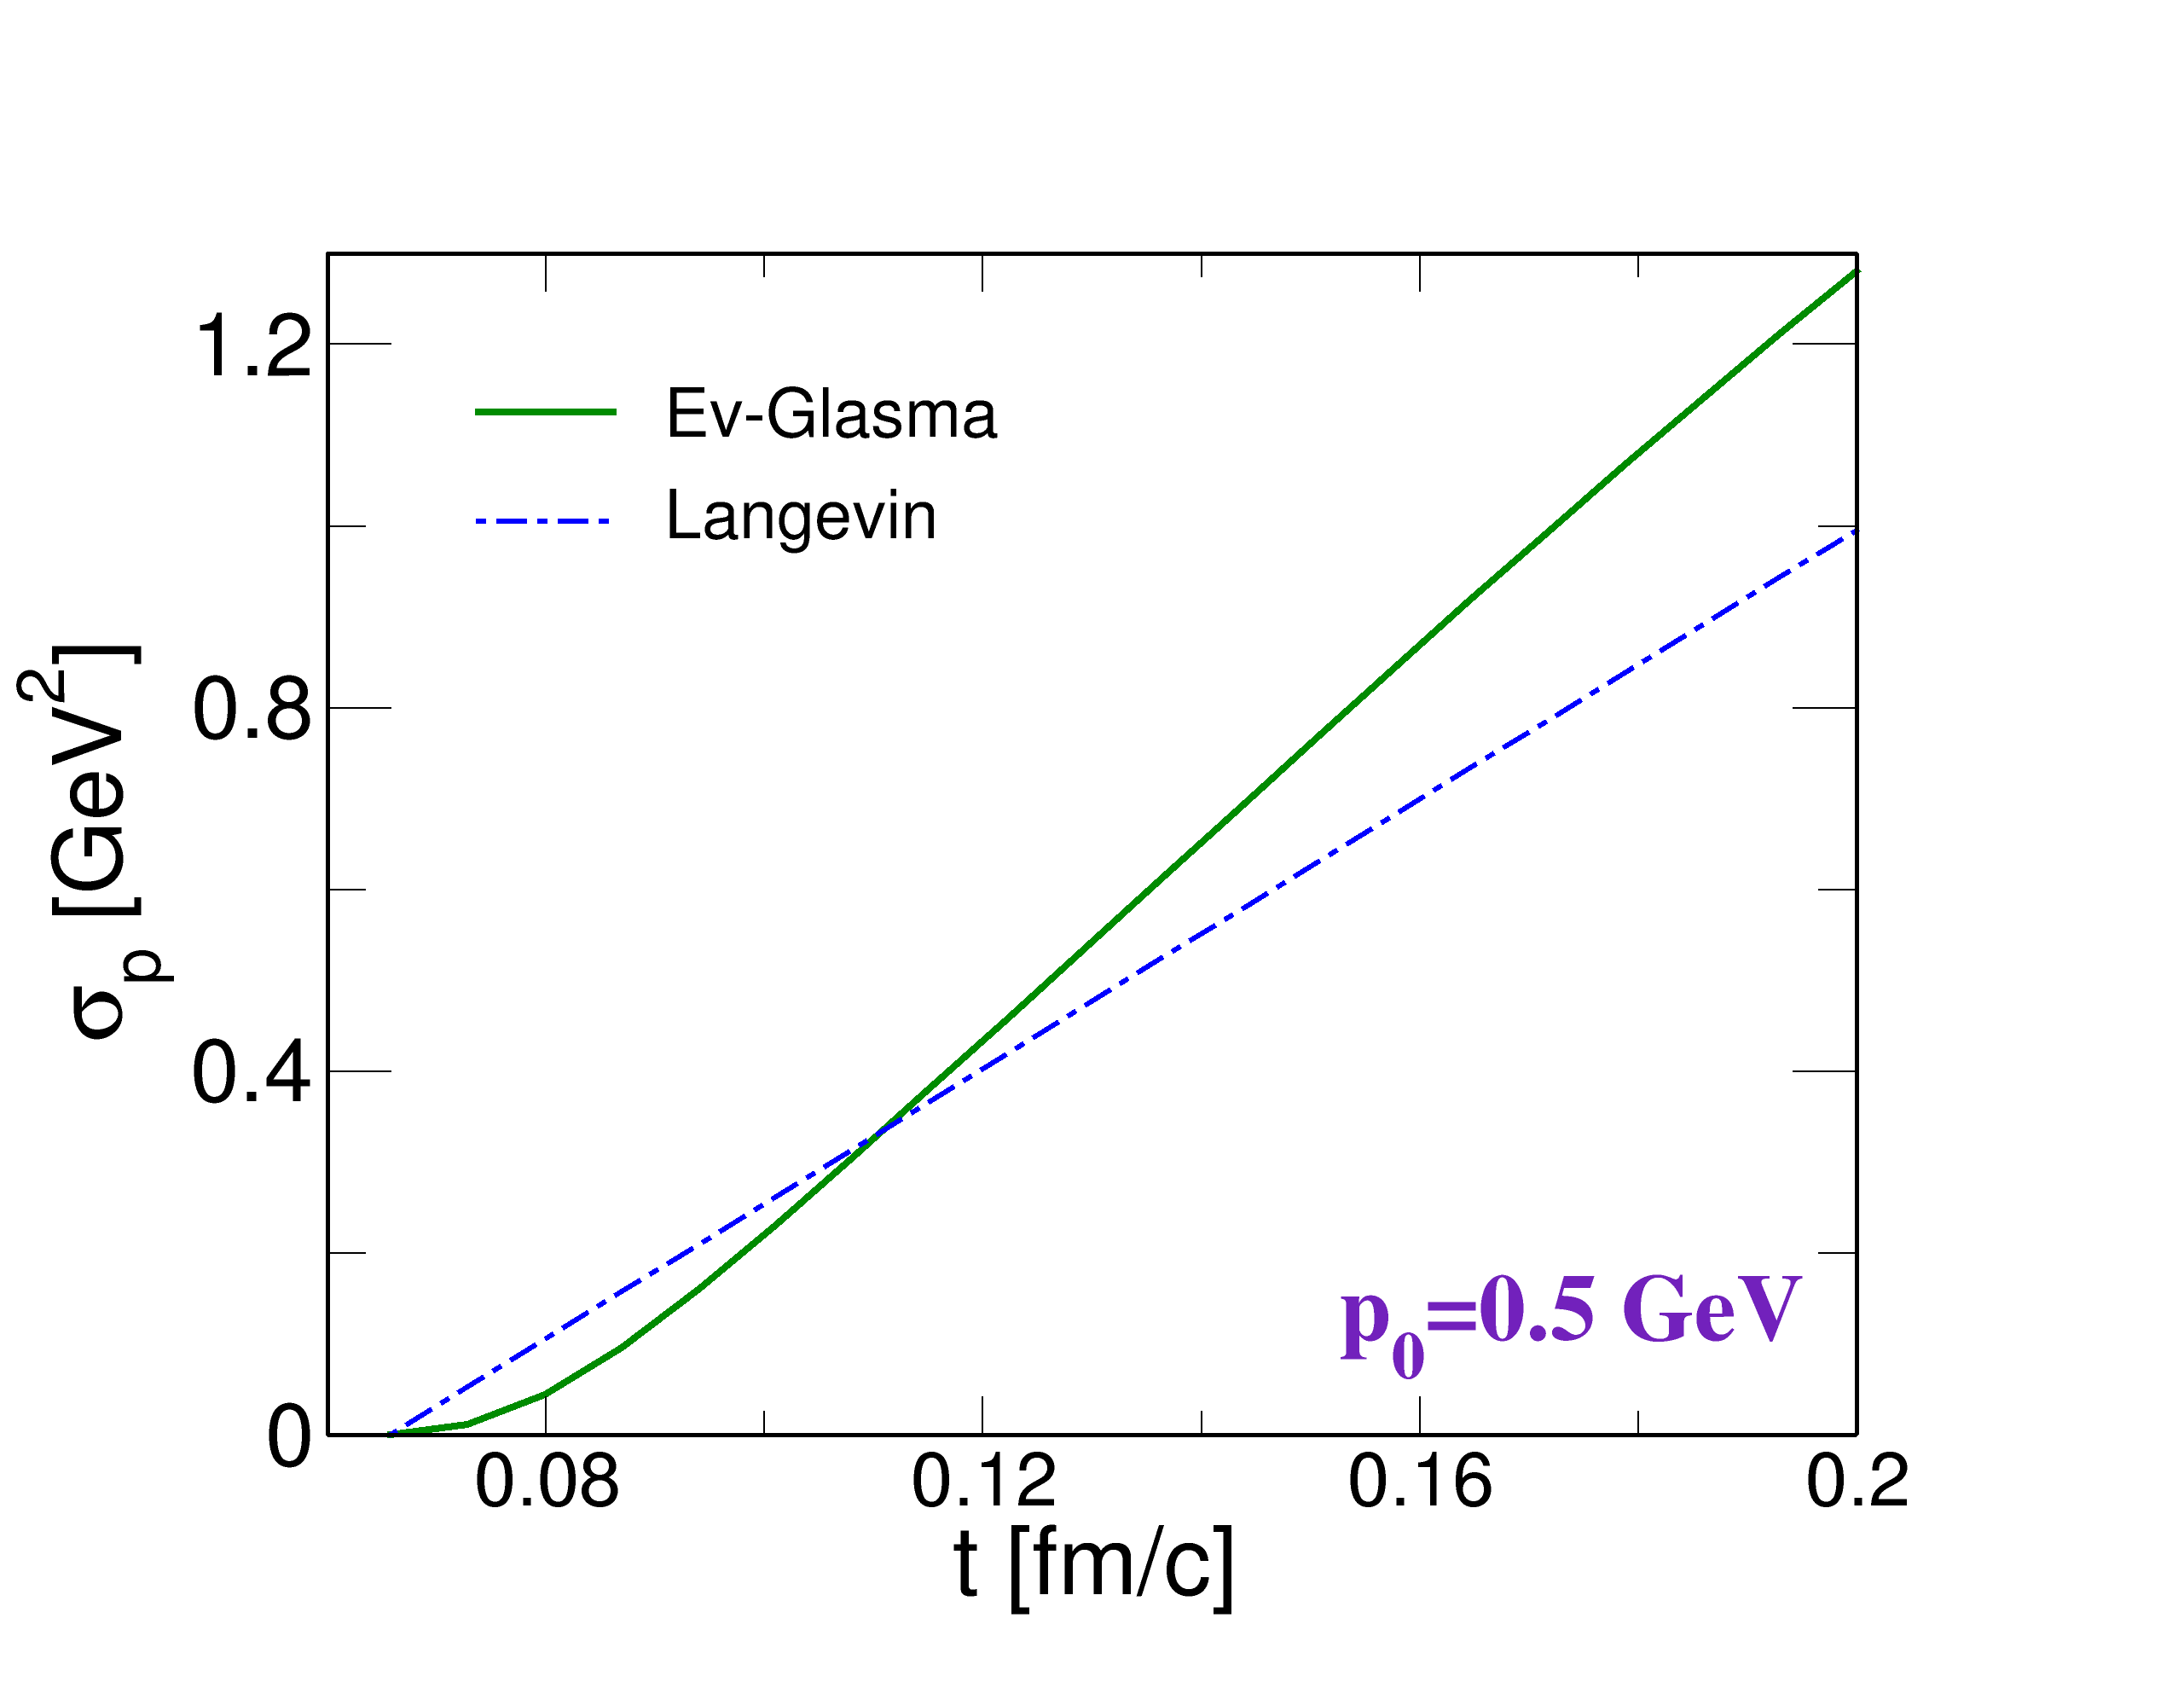
\includegraphics[width=0.95\textwidth]{images/zoom_02fm_langevin.png}}
%             \only<4>{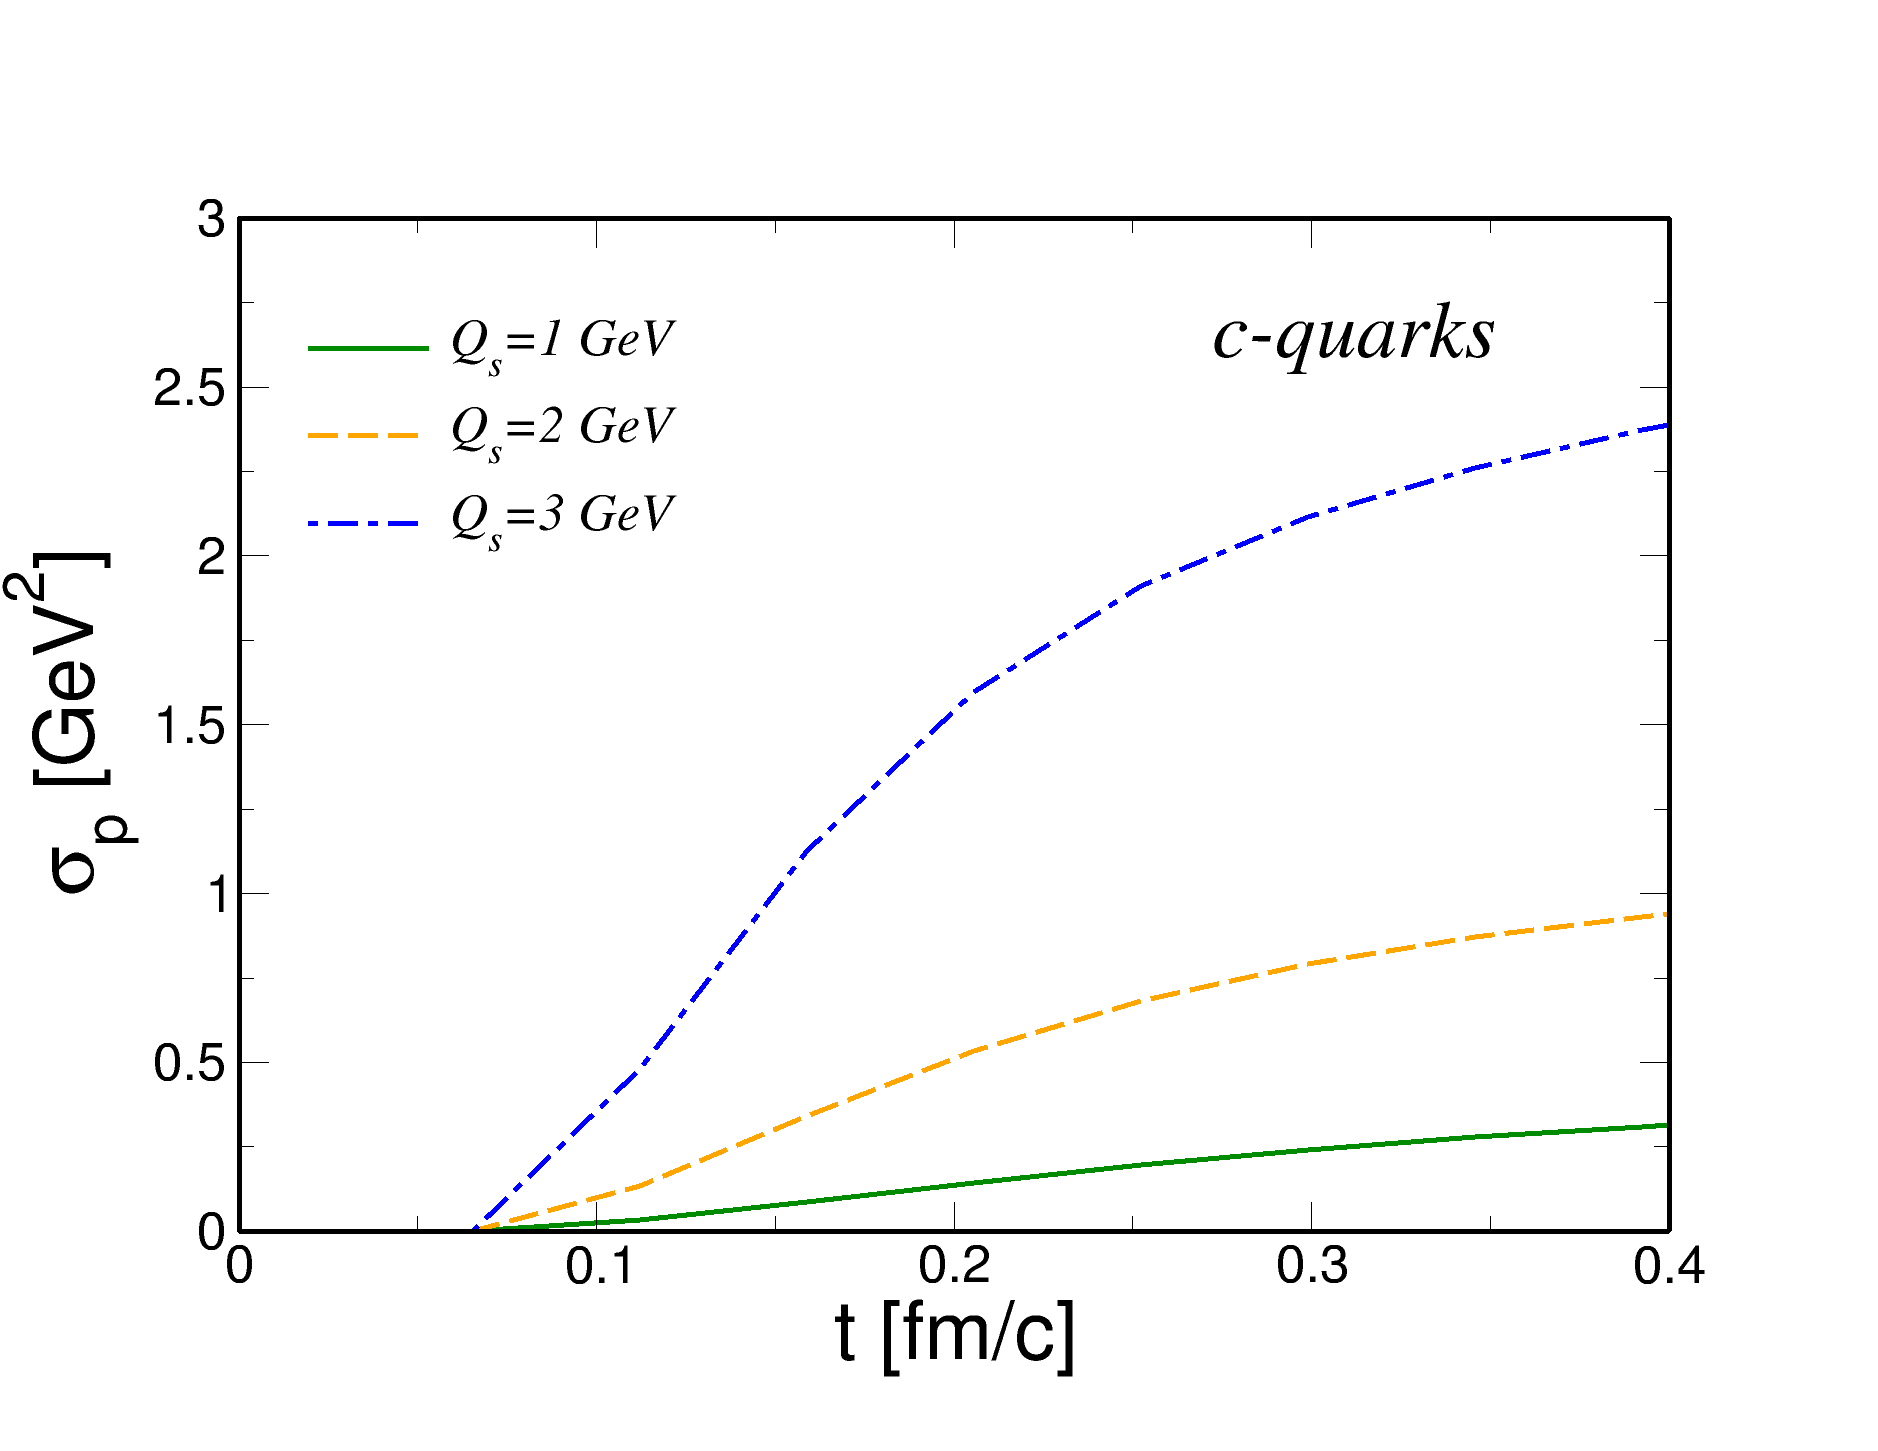
\includegraphics[width=0.95\textwidth]{images/sigmap_charm_expanding_04.png}}
%             \only<5>{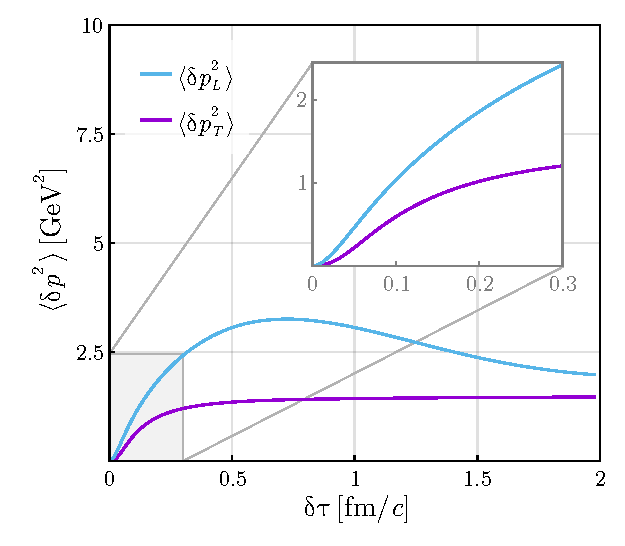
\includegraphics[width=0.9\textwidth]{images/beauty_early_behaviour_mom_broad.pdf}}
%             % \only<6>{\includegraphics[width=0.8\textwidth]{images/clean_raa_tau_0.3_charm_quark_Qs_2.0_fonll_pdf_vs_npdf_v3.png}}
%             % \only<7>{\includegraphics[width=0.8\textwidth]{images/final_dNdphi_tau_dep_charm_v2.png}}
%         \end{figure}
%         \column{.02\textwidth}
%         \column{.5\textwidth}
%         % \vspace{0.2cm}
%         \begin{center}
%             \begin{itemize}
%                 \only<1>{\item $R_{pA}$ for D-mesons\footnotemark \\[5pt] {\color{lightgray}\footnotesize First study in glasma\\ FONLL input + fragmentation\\
%                 SU(2) glasma, static box}}
%                 \only<2>{\item Hybrid $R_{AA}$ and $v_2$\footnotemark \\[5pt] {\color{lightgray}\footnotesize Compared with Fokker-Planck diffusion\\
%                 Glasma increases $v_2$ \\
%                 SU(2) glasma, static box 
%                 % \\[5pt]
%                 % Transport coefficients in QGP from {\color{jyured}Maria Lucia}}
%                 }}
%                 \only<3>{\item Momentum variance $\sigma_p$\footnotemark \\[5pt] {\color{lightgray}\footnotesize Compared with Langevin diffusion\\
%                 Glasma correlation domains\\
%                 SU(2) glasma, static box}}
%                 \only<4>{\item Momentum variance $\sigma_p$\footnotemark \\[5pt] {\color{lightgray}\footnotesize SU(2) glasma, longitudinal expansion}}
%                 \only<5>{\item Momentum broadening $\langle \delta p^2\rangle$\footnotemark\\
%                 Transport coefficient $\kappa$\footnotemark \\[5pt] {\color{lightgray}\footnotesize SU(3) glasma, longitudinal expansion\\
%                 Colored-particle-in-cell solver}}
%                 % \only<6>{\item $R_{AA}$ with nPDF effects \\[5pt] {\color{lightgray}\footnotesize FONLL + EPPS16 input calculation}}
%                 % \only<7>{\item Azimuthal decorrelation $\mathcal{C}(\Delta\phi)$ \\[5pt] {\color{lightgray}\footnotesize First study in glasma \\ $Q\overline{Q}$ pairs evolve in glasma}}
%             \end{itemize}
%         \end{center}
%         \column{.02\textwidth}
%     \end{columns}
%     \only<1>{\footnotetext{\scriptsize Ruggieri, Das \href{https://journals.aps.org/prd/abstract/10.1103/PhysRevD.98.094024}{{\color{customblue}\texttt{[Phys.Rev.D98(2018)]}}}}}
%     \only<2>{\footnotetext{\scriptsize Sun, Coci, Das, Plumari, Ruggieri, Greco \href{https://doi.org/10.1016/j.physletb.2019.134933}{{\color{customblue}\texttt{[Phys.Lett.B798(2019)]}}}}}
%     \only<3>{\footnotetext{\scriptsize Liu, Das, Greco, Ruggieri \href{https://journals.aps.org/prd/abstract/10.1103/PhysRevD.103.034029}{{\color{customblue}\texttt{[Phys.Rev.D103(2021)]}}}}}
%     \only<4>{\footnotetext{\scriptsize Khowal, Das, Oliva, Ruggieri \href{https://link.springer.com/article/10.1140/epjp/s13360-022-02517-w}{{\color{customblue}\texttt{[Eur.Phys.J.Plus137(2022)]}}}}}
%     \only<5>{\footnotetext{\scriptsize Avramescu, Băran, Greco, Ipp, Müller, Ruggieri  \href{https://journals.aps.org/prd/abstract/10.1103/PhysRevD.107.114021}{{\color{customblue}\texttt{[Phys.Rev.D107(2023)]}}}}}
%     % only<2>{\footnotetext{\scriptsize Sun, Coci, Das, Plumari, Ruggieri, Greco  \href{https://doi.org/10.1016/j.physletb.2019.134933}{{\color{customblue}\texttt{[Phys.Lett.B798(2019)]}}}}}
% \end{frame}

% \begin{frame}[noframenumbering]
%     \frametitle{Numerical trajectories results}
%     \begin{center}
%         \begin{tikzpicture}[xscale=1]%[scale=0.9, every node/.style={scale=0.6}]
%             \draw[line width=0.5mm,-latex,customblue!20] (-0.2,0) -- (8.5+0.2,0);
%             \foreach \X [evaluate=\X as \Y using int(\X-2017),count=\Z] in {2018, 2019, 2021, 2022}
%             {
%             \draw[highlight on=<0>] (\Y,0) circle[radius=2.5pt];
%             \node[anchor=south,highlight on=<0>,fill=white,rotate=45,anchor=south
%             west,inner sep=0pt] at (\Y,0.2) {\X};
%             }
%             \foreach \X [evaluate=\X as \Y using int(\X-2017),count=\Z] in {2024}
%             {
%             \draw[highlight on=<\Z>] (\Y,0) circle[radius=2.5pt];
%             \node[anchor=south,highlight on=<\Z>,fill=white,rotate=45,anchor=south
%             west,inner sep=0pt] at (\Y,0.2) {\X};
%             }
%         \end{tikzpicture}
%     \end{center}
%     \vspace{-10pt}
%     \begin{columns}[onlytextwidth,t]
%         \column{.02\textwidth}
%        \column{.44\textwidth}
%        \begin{figure}
%             \centering
%             \captionsetup{justification=centering}
%             \only<1>{\includegraphics[width=0.8\textwidth]{images/clean_raa_tau_0.3_charm_quark_Qs_2.0_fonll_pdf_vs_npdf_v3.png}}
%             % \only<7>{\includegraphics[width=0.8\textwidth]{images/final_dNdphi_tau_dep_charm_v2.png}}
%         \end{figure}
%         \column{.02\textwidth}
%         \column{.5\textwidth}
%         % \vspace{0.2cm}
%         \begin{center}
%             \begin{itemize}
%                 \only<1>{\item $R_{AA}$ with nPDF effects \\[5pt] {\color{lightgray}\footnotesize FONLL + EPPS16 input calculation}}
%                 % \only<7>{\item Azimuthal decorrelation $\mathcal{C}(\Delta\phi)$ \\[5pt] {\color{lightgray}\footnotesize First study in glasma \\ $Q\overline{Q}$ pairs evolve in glasma}}
%             \end{itemize}
%         \end{center}
%         \column{.02\textwidth}
%     \end{columns}
%     \only<1>{\footnotetext{\scriptsize Avramescu, Greco, Lappi, Mäntysaari, M\"{u}ller  {\color{customblue}\texttt{[in preparation]}}}}
% \end{frame}

% \begin{frame}[noframenumbering]
%     \frametitle{Numerical trajectories results}
%     \begin{center}
%         \begin{tikzpicture}[xscale=1]%[scale=0.9, every node/.style={scale=0.6}]
%             \draw[line width=0.5mm,-latex,customblue!20] (-0.2,0) -- (8.5+0.2,0);
%             \foreach \X [evaluate=\X as \Y using int(\X-2017),count=\Z] in {2018, 2019, 2021, 2022}
%             {
%             \draw[highlight on=<0>] (\Y,0) circle[radius=2.5pt];
%             \node[anchor=south,highlight on=<0>,fill=white,rotate=45,anchor=south
%             west,inner sep=0pt] at (\Y,0.2) {\X};
%             }
%             \foreach \X [evaluate=\X as \Y using int(\X-2017),count=\Z] in {2024}
%             {
%             \draw[highlight on=<\Z>] (\Y,0) circle[radius=2.5pt];
%             \node[anchor=south,highlight on=<\Z>,fill=white,rotate=45,anchor=south
%             west,inner sep=0pt] at (\Y,0.2) {\X};
%             }
%         \end{tikzpicture}
%     \end{center}
%     \vspace{-10pt}
%     \begin{columns}[onlytextwidth,t]
%         \column{.02\textwidth}
%        \column{.44\textwidth}
%        \begin{figure}
%             \centering
%             \captionsetup{justification=centering}
%             % \only<1>{\includegraphics[width=0.8\textwidth]{images/clean_raa_tau_0.3_charm_quark_Qs_2.0_fonll_pdf_vs_npdf_v3.png}}
%             \only<1>{\includegraphics[width=0.8\textwidth]{images/final_dNdphi_tau_dep_charm_v2.png}}
%         \end{figure}
%         \column{.02\textwidth}
%         \column{.5\textwidth}
%         % \vspace{0.2cm}
%         \begin{center}
%             \begin{itemize}
%                 % \only<1>{\item $R_{AA}$ with nPDF effects \\[5pt] {\color{lightgray}\footnotesize FONLL + EPPS16 input calculation}}
%                 \only<1>{\item Azimuthal decorrelation $\mathcal{C}(\Delta\phi)$ \\[5pt] {\color{lightgray}\footnotesize First study in glasma \\ $Q\overline{Q}$ pairs evolve in glasma}}
%             \end{itemize}
%         \end{center}
%         \column{.02\textwidth}
%     \end{columns}
%     \only<1>{\footnotetext{\scriptsize Avramescu, Greco, Lappi, Mäntysaari, M\"{u}ller  {\color{customblue}\texttt{[in preparation]}}}}
% \end{frame}


% \begin{frame}
%     \frametitle{Particles in Yang-Mills fields}
%     \framesubtitle{Correlator method}
%         \setbeamertemplate{itemize item}{\raisebox{0.2em}{\scalebox{0.7}{${\color{ming}\blacktriangleright}$}}} 
%         \begin{itemize}
%             \item \begin{center}{{\color{ming}Approach}: infer particle dynamics from background {\color{ming}field correlators}} \end{center}
%         \end{itemize} 
%         \renewcommand{\eqnhighlightheight}{\vphantom{x}}
%         \begin{equation*}
%             \langle \delta p^2_i(\tau)\rangle= g^2 \int\limits_{\tau_0}^{\tau}\mathrm{d}\tau^{\prime}\int\limits_{\tau_0}^{\tau}\mathrm{d}\tau^{\prime\prime}\eqnmark[ming]{FF}{\Big\langle \mathrm{Tr}\big[\widetilde{\mathcal{F}}_i(\tau^{\prime})\widetilde{\mathcal{F}}_i(\tau^{\prime\prime})\big]\Big\rangle}
%         \end{equation*}
%         \annotate[yshift=-1em]{below, left}{FF}{gauge invariant force correlator}
%         \\[20pt]
%         \begin{center}
%             {\footnotesize
%             Lorentz force $\mathcal{F}_i=F_{i\mu}\dfrac{p^\mu}{p^\tau}$ $\xrightarrow{\text{gauge invariant}}$ parallel transport on lattice $\widetilde{\mathcal{F}}_i$}
%         \end{center}

%         \begin{columns}
%             \begin{column}{0.033\textwidth}\end{column}
%             \begin{column}{0.45\textwidth}
%                 \centering
%                 \includegraphics[width=0.9\textwidth]{images/Picture9.pdf}
%             \end{column}
%             \begin{column}{0.01\textwidth}\end{column}
%             \begin{column}{0.45\textwidth}
%                 % \centering
%                 \vspace{-10pt}
%                 \setbeamertemplate{itemize item}{\raisebox{0.2em}{\scalebox{0.7}{${\color{customyellow}\blacktriangleright}$}}} 
%                 \begin{itemize}
%                     \item {\color{customyellow} Static heavy quarks} on lattice\footnotemark
%                 \end{itemize} 
%                 \vspace{10pt}
%                 {\footnotesize
%                 \begin{equation*}
%                     \langle \delta p^2_i(\tau)\rangle\big|_{\color{customyellow}m\rightarrow\infty}\propto \int_{\tau_0}^{\tau}\mathrm{d}\tau^{\prime}\int_{\tau_0}^{\tau}\mathrm{d}\tau^{\prime\prime}\Big\langle \mathrm{Tr}\big[{\color{customyellow}E_i}(\tau^{\prime}){\color{customyellow}E_i}(\tau^{\prime\prime})\big]\Big\rangle
%                 \end{equation*}}
%             \end{column}
%             \begin{column}{0.056\textwidth}\end{column}
%         \end{columns}
%         \footnotetext{Electric field correlators also used by {\color{jyured}Vijami} and {\color{jyured}Tom}}
% %    \begin{center}
% %        Wong's equations $\leftrightarrow$ classical equations of motion for particles $({\color{customblue}x^\mu},{\color{customred}p^\mu},{\color{customyellow}Q})$ \\
% %     evolving in a Yang-Mills background field ${\color{starrysecond}A^\mu}$
% %    \end{center} 
% %         \vspace{1cm}
% %         \renewcommand{\eqnhighlightheight}{\vphantom{x}}
% %         \begin{equation*}
% %             \frac{\d}{\d\hspace{-0.1cm}\eqnmark[destacado]{tau}{\boldsymbol{\tau}}\hspace{-0.2cm}}\eqnmark[customblue]{xmu}{x^\mu}=\frac{{\color{customred}p^\mu}}{\eqnmark[destacado]{m}{m}},\qquad \eqnmark[destacado]{Ddtau}{\frac{\mathrm{D}}{\d\boldsymbol{\tau}}}\hspace{-0.2cm}\eqnmark[customred]{pmu}{p^\mu}=2\hspace{-0.1cm}\eqnmark[destacado]{g}{g}\hspace{-0.1cm}\tr{{\color{customyellow}Q}F^{\mu\nu}[\hspace{-0.1cm}\eqnmark[starrysecond]{amu}{A^\mu}\hspace{-0.1cm}]}\frac{{\color{customred}p_\nu}}{m},\qquad 
% %             \underbrace{\frac{\d}{\d\boldsymbol{\tau}}\hspace{-0.1cm}\eqnmark[customyellow]{Q}{Q}\hspace{-0.1cm}=-\mathrm{i}g [{\color{starrysecond}A_\mu},{\color{customyellow}Q}]\,\frac{{\color{customred}p^\mu}}{m}}_{\substack{\text{\footnotesize color rotation}\,\rightarrow\,{\color{customgreen}\mathcal{U}}\in\,\mathrm{SU(3)} \\[0.2cm] {\color{customyellow}Q}(\boldsymbol{\tau})=\,{\color{customgreen}\mathcal{U}}(\boldsymbol{\tau},\boldsymbol{\tau}^\prime){\color{customyellow}Q}(\boldsymbol{\tau^\prime})\,{\color{customgreen}\mathcal{U}^\dagger}(\boldsymbol{\tau},\boldsymbol{\tau}^\prime)}}
% %             \end{equation*}
% %             \annotate[yshift=1.2em]{above}{xmu}{coordinate}
% %             \annotate[yshift=1.2em]{above}{pmu}{momentum}
% %             \annotate[yshift=-0.5em]{below, right}{m}{\tiny mass}
% %             \annotate[yshift=-1.5em]{below, right}{Ddtau}{\tiny covariant derivative}
% %             \annotate[yshift=-1.5em]{below, right}{tau}{\tiny proper time}
% %             \annotate[yshift=-0.7em]{below, right}{g}{\tiny coupling constant}
% %             \annotate[yshift=1.2em]{above}{Q}{color charge}
% %             \annotate[yshift=1.2em]{above, right}{amu}{gauge field}
%     %    \\
%         % \begin{center}
%         %     Symplectic numerical solver $\xrightarrow{\mathrm{assures}}$ ${\color{customyellow}Q}\in\mathrm{SU(3)}$, conservation of Casimir invariants 
%         % \end{center} 
% \end{frame}



% \begin{frame}[t]
%     \frametitle{Field correlators results}
%     \begin{center}
%         \begin{tikzpicture}[xscale=1]
%             \draw[line width=0.5mm,-latex,customblue!20] (-0.2,0) -- (6.5+0.2,0);
%             \foreach \X [evaluate=\X as \Y using int(\X-2019),count=\Z] in {2023, 2024}
%             {
%             \draw[highlight on=<0>] (\Y,0) circle[radius=2.5pt];
%             \node[anchor=south,highlight on=<0>,fill=white,rotate=45,anchor=south
%             west,inner sep=0pt] at (\Y,0.2) {\X};
%             }
%             \foreach \X [evaluate=\X as \Y using int(\X-2019),count=\Z] in {2020}
%             {
%             \draw[highlight on=<\Z>] (\Y,0) circle[radius=2.5pt];
%             \node[anchor=south,highlight on=<\Z>,fill=white,rotate=45,anchor=south
%             west,inner sep=0pt] at (\Y,0.2) {\X};
%             }
%         \end{tikzpicture}
%     \end{center}
%     \vspace{-10pt}
%     \begin{columns}[onlytextwidth,t]
%         \column{.02\textwidth}
%        \column{.44\textwidth}
%        \begin{figure}
%             \centering
%             \captionsetup{justification=centering}
%             \only<1>{\includegraphics[width=0.9\textwidth]{images/1-s2.0-S0375947420302244-gr003_lrg (2).jpg}}
%         \end{figure}
%         \column{.02\textwidth}
%         \column{.5\textwidth}
%         % \vspace{0.2cm}
%         \begin{center}
%             \begin{itemize}
%                 \only<1>{\item Transport coefficient $\kappa$ \\ Collisional energy loss $\mathrm{d}E/\mathrm{d}x$ \\[5pt] {\color{lightgray}\footnotesize Analytical glasma fields in $\tau$ expansion \\
%                 Glasma $E$ and $B$ field correlators \\
%                 Fokker-Planck equation for heavy quarks \\
%                 }}
%             \end{itemize}
%         \end{center}
%         \column{.02\textwidth}
%     \end{columns}
%     \only<1>{\footnotetext{\scriptsize Carrington, Czajka, Mrowczynski \href{https://doi.org/10.1016/j.nuclphysa.2020.121914}{\color{customblue}\texttt{[Nucl.Phys.A1001(2020)]}}}}
% \end{frame}



% \begin{frame}[noframenumbering]
%     \frametitle{Field correlators results}
%     \begin{center}
%         \begin{tikzpicture}[xscale=1]
%             \draw[line width=0.5mm,-latex,customblue!20] (-0.2,0) -- (6.5+0.2,0);
%             \foreach \X [evaluate=\X as \Y using int(\X-2019),count=\Z] in {2023, 2024}
%             {
%             \draw[highlight on=<0>] (\Y,0) circle[radius=2.5pt];
%             \node[anchor=south,highlight on=<0>,fill=white,rotate=45,anchor=south
%             west,inner sep=0pt] at (\Y,0.2) {\X};
%             }
%             \foreach \X [evaluate=\X as \Y using int(\X-2019),count=\Z] in {2020}
%             {
%             \draw[highlight on=<\Z>] (\Y,0) circle[radius=2.5pt];
%             \node[anchor=south,highlight on=<\Z>,fill=white,rotate=45,anchor=south
%             west,inner sep=0pt] at (\Y,0.2) {\X};
%             }
%         \end{tikzpicture}
%     \end{center}
%     \vspace{-10pt}
%     \begin{columns}[onlytextwidth,t]
%         \column{.02\textwidth}
%        \column{.44\textwidth}
%        \begin{figure}
%             \centering
%             \captionsetup{justification=centering}
%             \only<1>{\includegraphics[width=0.85\textwidth]{images/mombroadening_with_inset_and_approximations.pdf}}
%         \end{figure}
%         \column{.02\textwidth}
%         \column{.5\textwidth}
%         % \vspace{0.2cm}
%         \begin{center}
%             \begin{itemize}
%                 \only<1>{\item Momentum broadening $\langle \delta p^2 \rangle$ \\ Transport coefficient $\kappa$ \\[5pt] {\color{lightgray}\footnotesize Over-occupied classical Yang-Mills \\
%                 Numerical lattice $\langle EE\rangle$ correlator \\
%                 Large peak in $\langle \delta p^2 \rangle$ \\
%                 Oscillations of $\kappa$ with plasmon frequency
%                 }}
%             \end{itemize}
%         \end{center}
%         \column{.02\textwidth}
%     \end{columns}
%     \only<1>{\footnotetext{\scriptsize Boguslavski, Kurkela, Lappi, Peuron \href{https://doi.org/10.1007/JHEP09(2020)077}{\color{customblue}\texttt{[JHEP09(2020)]}}}}
% \end{frame}




% \begin{frame}[noframenumbering]
%     \frametitle{Field correlators results}
%     \begin{center}
%         \begin{tikzpicture}[xscale=1]
%             \draw[line width=0.5mm,-latex,customblue!20] (-0.2,0) -- (6.5+0.2,0);
%             \foreach \X [evaluate=\X as \Y using int(\X-2019),count=\Z] in {2020, 2024}
%             {
%             \draw[highlight on=<0>] (\Y,0) circle[radius=2.5pt];
%             \node[anchor=south,highlight on=<0>,fill=white,rotate=45,anchor=south
%             west,inner sep=0pt] at (\Y,0.2) {\X};
%             }
%             \foreach \X [evaluate=\X as \Y using int(\X-2019),count=\Z] in {2023}
%             {
%             \draw[highlight on=<\Z>] (\Y,0) circle[radius=2.5pt];
%             \node[anchor=south,highlight on=<\Z>,fill=white,rotate=45,anchor=south
%             west,inner sep=0pt] at (\Y,0.2) {\X};
%             }
%         \end{tikzpicture}
%     \end{center}
%     \vspace{-10pt}
%     \begin{columns}[onlytextwidth,t]
%         \column{.02\textwidth}
%        \column{.44\textwidth}
%        \begin{figure}
%             \centering
%             \captionsetup{justification=centering}
%             \only<1>{\includegraphics[width=0.8\textwidth]{images/hp23_mom_broad_kappa_anis_wong_vs_kappa-cropped.pdf}}
%         \end{figure}
%         \column{.02\textwidth}
%         \column{.5\textwidth}
%         % \vspace{0.2cm}
%         \begin{center}
%             \begin{itemize}
%                 \only<1>{\item Momentum broadening $\langle \delta p^2 \rangle$ \\ Transport coefficient $\kappa$ \\[5pt] {\color{lightgray}\footnotesize Numerical lattice $\langle EE\rangle$ correlator \\ 
%                 Comparison with numerical trajectories \\
%                 Ordering $\langle\delta p^2_L\rangle>\langle\delta p^2_T\rangle$, negative $\kappa_L<0$ 
%                 }}
%             \end{itemize}
%         \end{center}
%         \column{.02\textwidth}
%     \end{columns}
%     \only<1>{\footnotetext{\scriptsize Avramescu, Băran, Greco, Ipp, Müller, Ruggieri  \href{https://pos.sissa.it/438/056}{{\color{customblue}\texttt{[PoSHardProbes2023(2024)]}}}}}
% \end{frame}


% \begin{frame}[noframenumbering]
%     \frametitle{Field correlators results}
%     \begin{center}
%         \begin{tikzpicture}[xscale=1]
%             \draw[line width=0.5mm,-latex,customblue!20] (-0.2,0) -- (6.5+0.2,0);
%             \foreach \X [evaluate=\X as \Y using int(\X-2019),count=\Z] in {2020, 2023}
%             {
%             \draw[highlight on=<0>] (\Y,0) circle[radius=2.5pt];
%             \node[anchor=south,highlight on=<0>,fill=white,rotate=45,anchor=south
%             west,inner sep=0pt] at (\Y,0.2) {\X};
%             }
%             \foreach \X [evaluate=\X as \Y using int(\X-2019),count=\Z] in {2024}
%             {
%             \draw[highlight on=<\Z>] (\Y,0) circle[radius=2.5pt];
%             \node[anchor=south,highlight on=<\Z>,fill=white,rotate=45,anchor=south
%             west,inner sep=0pt] at (\Y,0.2) {\X};
%             }
%         \end{tikzpicture}
%     \end{center}
%     \vspace{-10pt}
%     \begin{columns}[onlytextwidth,t]
%         \column{.02\textwidth}
%        \column{.44\textwidth}
%        \begin{figure}
%             \centering
%             \captionsetup{justification=centering}
%             \only<1>{\includegraphics[width=0.9\textwidth]{images/2Dsc_g_SR_Qt500.pdf}}
%         \end{figure}
%         \column{.02\textwidth}
%         \column{.5\textwidth}
%         % \vspace{0.2cm}
%         \begin{center}
%             \begin{itemize}
%                 \only<1>{\item Transport coefficient $\kappa$ \\[5pt] {\color{lightgray}\footnotesize 
%                 Glasma-like classical fields \\
%                 Numerical lattice $\langle EE\rangle$ correlator \\ 
%                 Effect of non-perturbative gluonic excitations \\
%                 Explain the peak in $\kappa$
%                 }}
%             \end{itemize}
%         \end{center}
%         \column{.02\textwidth}
%     \end{columns}
%     \only<1>{\footnotetext{\scriptsize Backfried, Boguslavski, Hotzy \href{https://arxiv.org/abs/2408.12646}{{\color{customblue}\texttt{[arXiv2408.12646]}}}}}
% \end{frame}


    
% % \begin{frame}[t]
% %     \frametitle{Historial}
% %     \begin{tikzpicture}[xscale=0.5]
% %     \draw[line width=0.5mm,-latex,customblue!20] (-0.2,0) -- (20+0.2,0);
% %     \foreach \X [evaluate=\X as \Y using int(\X-2000),count=\Z] in {2000,2001,2002} %<- these are the years not to be highlighted
% %     {
% %     % \draw[highlight on=<0>] ({\Y-0.2},-0.5) -- ({\Y+0.2},-0.5) -- (\Y,-0.1) -- cycle;
% %     \node[circle, highlight on=<\Z>,inner sep=2pt,color=customblue] at (\Y,0) {};
% %     \node[anchor=south,highlight on=<0>,fill=white,rotate=45,anchor=south
% %     west,inner sep=0pt] at (\Y,0.2) {\X};
% %     }
% %     \foreach \X [evaluate=\X as \Y using int(\X-2000),count=\Z] in {2005,2008,2015} %<- these are the years which are to be highlighted
% %     {
% %     % \draw[highlight on=<\Z>] ({\Y-0.2},-0.5) -- ({\Y+0.2},-0.5) -- (\Y,-0.1) -- cycle;
% %     \node[circle, highlight on=<\Z>,inner sep=2pt,color=customblue] at (\Y,0) {};
% %     \node[anchor=south,highlight on=<\Z>,fill=white,rotate=45,anchor=south
% %     west,inner sep=0pt] at (\Y,0.2) {\X};
% %     }
% %     \end{tikzpicture}
% %     \begin{itemize}
% %         \item<1> November 2005: marmots start hibernating again
% %     \end{itemize}
% % \end{frame}



% \subsection{Kinetic theory}
% \setbeamertemplate{background}{
% \tikz[overlay,remember picture] \node[opacity=0.1, at=(current page.center), align=center] {\\[10pt]
% {\transparent{0.1}\includegraphics[height=0.7\paperheight]{images/heavy-ion3.pdf}}
%    \\[10pt]  
%    {\transparent{0.3}\footnotesize\itshape Figure from  K. Boguslavski, A. Kurkela, T. Lappi, F. Lindenbauer, J. Peuron \href{https://arxiv.org/abs/2312.00447}{{\color{lightgray}\texttt{[2312.00447]}}}}};
% }
% % \begin{frame}[plain,noframenumbering]{}
% %     \begin{center}
% %         \vspace{1cm}
% %         {\large\color{normal}Next stages of pre-equilibrium}\\[0.3cm]
% %         {\huge\color{destacado}Thermalization of heavy quarks}
% %     \end{center}
% % \end{frame}
% % \setbeamertemplate{background}{}

% \begin{frame}[plain,noframenumbering]{}
%     \begin{center}
%         \vspace{1cm}
%         {\large\color{normal}Next stages of pre-equilibrium}\\[0.3cm]
%         {\huge\color{destacado}Heavy quarks during bottom-up}\\[0.3cm]
%         {\large\color{normal}
%         \begin{center}
%             % \begin{minipage}{0.45\textwidth}
%             % \begin{itemize}
%             %     \item Momentum broadening $\langle \delta p^2\rangle$
%             %     \item Transport coefficient $\kappa$
%             %     \item Observables $R_{AA}$, $v_2$, $\mathcal{C}(\Delta\phi)$
%             % \end{itemize}
%             % \end{minipage}
%             \begin{columns}
%                 \begin{column}{0.066\textwidth}\end{column}
%                 \begin{column}{0.35\textwidth}
%                     \centering
%                     \setbeamertemplate{itemize item}{\raisebox{0.2em}{\scalebox{0.7}{${\color{ming}\blacktriangleright}$}}} 
%                     {\Large\color{ming} Approaches}
%                     \begin{itemize}
%                         \item Effective kinetic theory
%                     \end{itemize}
%                 \end{column}
%                 \begin{column}{0.066\textwidth}\end{column}
%                 \begin{column}{0.45\textwidth}
%                     \centering
%                     \\[10pt]
%                     \setbeamertemplate{itemize item}{\raisebox{0.2em}{\scalebox{0.7}{${\color{pinky}\blacktriangleright}$}}} 
%                     {\Large\color{pinky} Quantities}
%                     \begin{itemize}
%                         \item Transport coefficient $\kappa$
%                         \item Drag, diffusion coefficients $A_i$, $B_{ij}$
%                     \end{itemize}
%                 \end{column}
%                 \begin{column}{0.066\textwidth}\end{column}
%             \end{columns}
%         \end{center}
%         }
%         % \\[0.3cm]
%     \end{center}
% \end{frame}
% \setbeamertemplate{background}{}



% \begin{frame}
%     \frametitle{Heavy quarks in EKT}
%     \framesubtitle{Extracting transport coefficients}
%         \setbeamertemplate{itemize item}{\raisebox{0.2em}{\scalebox{0.7}{${\color{ming}\blacktriangleright}$}}}
%         \vspace{10pt} 
%         \begin{itemize}
%             \item \begin{center}{{\color{ming}Approach}: {\color{ming}effective kinetic theory} $\rightarrow$ gluon distribution function $f(\boldsymbol{k})$} \end{center}
%         \end{itemize} 
% %    \begin{center}
% %        Wong's equations $\leftrightarrow$ classical equations of motion for particles $({\color{customblue}x^\mu},{\color{customred}p^\mu},{\color{customyellow}Q})$ \\
% %     evolving in a Yang-Mills background field ${\color{starrysecond}A^\mu}$
% %    \end{center} 
%         \begin{columns}
%             \begin{column}{0.066\textwidth}\end{column}
%             \begin{column}{0.35\textwidth}
%                 \centering
%                 \begin{figure}
%                     \centering
%                     \captionsetup{justification=centering}
%                     \includegraphics[width=0.9\textwidth]{images/feynmandiag_wo_title.pdf}
%                     \caption{\scriptsize Figure credits to F. Lindenbauer}
%                 \end{figure}
%             \end{column}
%             \begin{column}{0.033\textwidth}\end{column}
%             \begin{column}{0.483\textwidth}
%                 % \vspace{1cm}
%                 \renewcommand{\eqnhighlightheight}{\vphantom{x}}
%                 \begin{equation*}
%                     \kappa\propto \int\eqnmark[starrysecond]{PS}{\mathrm{d}\Gamma_{\mathrm{PS}}}\hspace{-2pt}\eqnmark[pinky]{q}{\boldsymbol{q}^2}\hspace{-2pt}\abs{\hspace{-2pt}\eqnmark[ektblue]{M}{\mathcal{M}}\hspace{-2pt}}^2f(\hspace{-3pt}\eqnmark[ektgreen]{fk}{\boldsymbol{k}}\hspace{-3pt})[1+f(\hspace{-3pt}\eqnmark[ektgreen]{fkp}{\boldsymbol{k}^{\boldsymbol{\prime}}}\hspace{-3pt})]
%                     \end{equation*}
%                     \annotate[yshift=+2.0em]{above, right}{PS}{\tiny phase space measure}
%                     \annotate[yshift=+0.5em]{above, right}{M}{\tiny matrix element}
%                     \annotate[yshift=-2.0em]{below, right}{q}{\tiny momentum exchange}
%                     \annotate[yshift=-0.5em]{below, right}{fk}{\tiny incoming}
%                     \annotate[yshift=-0.5em]{below, right}{fkp}{\tiny outgoing}
%             \end{column}
%             \begin{column}{0.066\textwidth}\end{column}
%         \end{columns}
%         \vspace{-5pt}
%         \begin{center}
%             \footnotesize
%             \hspace{9pt}Drag $\displaystyle A_i\propto \int\mathrm{d}\Gamma_{\mathrm{PS}}\,\boldsymbol{q}_i\,\abs{\mathcal{M}}^2f(\boldsymbol{k})[1\pm f(\boldsymbol{k}^{\boldsymbol{\prime}})]$ \\
%             Diffusion $\displaystyle B_{ij}\propto \int\mathrm{d}\Gamma_{\mathrm{PS}}\,\boldsymbol{q}_i\boldsymbol{q}_j\,\abs{\mathcal{M}}^2f(\boldsymbol{k})[1\pm f(\boldsymbol{k}^{\boldsymbol{\prime}})]$
%         \end{center}

%         % \begin{center}
%         %     Symplectic numerical solver $\xrightarrow{\mathrm{assures}}$ ${\color{customyellow}Q}\in\mathrm{SU(3)}$, conservation of Casimir invariants 
%         % \end{center} 
% \end{frame}


% \begin{frame}[t]
%     \frametitle{EKT results}
%     \begin{center}
%         \begin{tikzpicture}[xscale=1]
%             \draw[line width=0.5mm,-latex,customblue!20] (-0.2,0) -- (2.5+0.2,0);
%             \foreach \X [evaluate=\X as \Y using int(\X-2023),count=\Z] in {2024}
%             {
%             \draw[highlight on=<\Z>] (\Y,0) circle[radius=2.5pt];
%             \node[anchor=south,highlight on=<\Z>,fill=white,rotate=45,anchor=south
%             west,inner sep=0pt] at (\Y,0.2) {\X};
%             }
%         \end{tikzpicture}
%     \end{center}
%     \vspace{-10pt}
%     \begin{columns}[onlytextwidth,t]
%         \column{.02\textwidth}
%        \column{.44\textwidth}
%        \begin{figure}
%             \centering
%             \captionsetup{justification=centering}
%             \only<1>{\includegraphics[width=0.9\textwidth]{images/KappaGlasmaVsEKTvsLatticev2.pdf}}
%         \end{figure}
%         \column{.02\textwidth}
%         \column{.5\textwidth}
%         % \vspace{0.2cm}
%         \begin{center}
%             \begin{itemize}
%                 \only<1>{\item Transport coefficient $\kappa$ \\[5pt] 
%                 {\color{lightgray}\footnotesize Compare to $\kappa$ in glasma \\
%                 Compare with equilibrium $\kappa_{\mathrm{eq}}$ \\
%                 Match for the same $m_D$, $T_{\star}$ and $\varepsilon$
%                 }
%                 }
%             \end{itemize}
%         \end{center}
%         \column{.02\textwidth}
%     \end{columns}
%     \only<1>{\footnotetext{\scriptsize Boguslavski, Kurkela, Lappi, Lindenbauer, Peuron \href{https://journals.aps.org/prd/abstract/10.1103/PhysRevD.109.014025}{\color{customblue}\texttt{[Phys.Rev.D109(2024)]}}}}
% \end{frame}


% \begin{frame}[noframenumbering]
%     \frametitle{EKT results}
%     \begin{center}
%         \begin{tikzpicture}[xscale=1]
%             \draw[line width=0.5mm,-latex,customblue!20] (-0.2,0) -- (2.5+0.2,0);
%             \foreach \X [evaluate=\X as \Y using int(\X-2023),count=\Z] in {2024}
%             {
%             \draw[highlight on=<\Z>] (\Y,0) circle[radius=2.5pt];
%             \node[anchor=south,highlight on=<\Z>,fill=white,rotate=45,anchor=south
%             west,inner sep=0pt] at (\Y,0.2) {\X};
%             }
%         \end{tikzpicture}
%     \end{center}
%     \vspace{-10pt}
%     \begin{columns}[onlytextwidth,t]
%         \column{.02\textwidth}
%        \column{.44\textwidth}
%        \begin{figure}
%             \centering
%             \captionsetup{justification=centering}
%             \only<1>{\includegraphics[width=0.9\textwidth]{images/Ai_t.pdf}}
%         \end{figure}
%         \column{.02\textwidth}
%         \column{.5\textwidth}
%         % \vspace{0.2cm}
%         \begin{center}
%             \begin{itemize}
%                 \only<1>{\item Drag, diffusion $A_i$, $B_{ij}$ \\[5pt] 
%                 {\color{lightgray}\footnotesize Contributions from $g, q, g+q$ \\
%                 Angular dependence \\
%                 Rescaled coefficients, attractor behavior
%                 }
%                 }
%             \end{itemize}
%         \end{center}
%         \column{.02\textwidth}
%     \end{columns}
%     \only<1>{\footnotetext{\scriptsize Du \href{https://journals.aps.org/prc/abstract/10.1103/PhysRevC.109.014901}{\color{customblue}\texttt{[Phys.Rev.C109(2024)]}}}}
% \end{frame}



% %%%%%%%%%%%%%%%%%%%%%%%%%%%%%%%%%%%%%%%%%%%
% %%%%%%%%%%%%%%%% SECTION 4 %%%%%%%%%%%%%%%%
% %%%%%%%%%%%%%%%%%%%%%%%%%%%%%%%%%%%%%%%%%%%

% \section{Open questions}

% \begin{frame}
%     \frametitle{Open questions}
%     % \framesubtitle{Wong's equations of motion} 
%         \begin{itemize}
%             % \setbeamertemplate{itemize item}{\raisebox{0.2em}{\scalebox{0.7}{${\color{ming}\blacktriangleright}$}}}
%             % \item {\large{{\color{ming}Approach}: {\color{ming}numerical trajectories} of classical particles in glasma fields}}
%             \setbeamertemplate{itemize item}{\raisebox{0.2em}{\scalebox{0.7}{${\color{ming}\blacktriangleright}$}}}
%             \item  {\large{Theoretical improvements}}
%                 % \\[10pt]
%                 \begin{itemize}
%                     \item[\raisebox{0.2em}{\scalebox{0.6}{${\color{ming}\blacktriangleright}$}}] First stage of bottom-up thermalization\\
%                     {\scriptsize\color{lightgray}How to connect $\kappa$ from glasma to EKT? Match using gluon distribution function} \\[5pt]
%                     \item[\raisebox{0.2em}{\scalebox{0.6}{${\color{ming}\blacktriangleright}$}}] Heavy quark energy loss in glasma \\
%                     {\scriptsize\color{lightgray}Only recently: jet energy loss in glasma from synchrotron radiation {\color{jyured}Add reference}}
%                 \end{itemize}
%                 % \\[10pt]
%             \setbeamertemplate{itemize item}{\raisebox{0.2em}{\scalebox{0.7}{${\color{pinky}\blacktriangleright}$}}}
%                 \item  {\large{Experimental observables}}
%                 % \\[10pt]
%                 \begin{itemize}
%                     \item[\raisebox{0.2em}{\scalebox{0.6}{${\color{pinky}\blacktriangleright}$}}] Observables sensitive to pre-equilibrium\\
%                     {\scriptsize\color{lightgray}What to extract? The most sensitive is the azimuthal correlation} \\[5pt]
%                     \item[\raisebox{0.2em}{\scalebox{0.6}{${\color{pinky}\blacktriangleright}$}}] Large initial anisotropy \\
%                     {\scriptsize\color{lightgray}How to measure anisotropy $\rightarrow$ many studies in anisotropic systems {\color{jyured}Add references}}
%                 \end{itemize}
%             %     \\[10pt] 
%                 \setbeamertemplate{itemize item}{\raisebox{0.2em}{\scalebox{0.7}{${\color{jyured}\blacktriangleright}$}}}
%                 \item  {\large{Compare theory to experiment}}
%                 % \\[10pt]
%                 \begin{itemize}
%                     \item[\raisebox{0.2em}{\scalebox{0.6}{${\color{jyured}\blacktriangleright}$}}] {\scriptsize\color{lightgray} How sensitive is data to pre-equilibrium? Simulations of all stages for HQ transport
%                     }
%                 \end{itemize}
%             %     % \\[10pt] 
%         \end{itemize} 
% \end{frame}


\end{document}